% ------------------------------------------------------------
% LaTeX Template für die DHBW zum Schnellstart!
% Original: https://github.wdf.sap.corp/vtgermany/LaTeX-Template-DHBW
% ------------------------------------------------------------
% ---- Präambel mit Angaben zum Dokument
\input{Inhalt/00_Latex/praeambel}

% ---- Elektronische Version oder Gedruckte Version?
% ---- Unterschied: Die elektronische Version enthält keinen Platzhalter für die Unterschrift
\usepackage{ifthen}
\newboolean{e-Abgabe}
\setboolean{e-Abgabe}{false}    % false=gedruckte Fassung

% ---- Persönlichen Daten:
\newcommand{\titel}{Softwareentwurf Advanced SWE}
\newcommand{\titelheader}{Softwareentwurf Advanced SWE}
\newcommand{\arbeit}{Softwareentwurf}
\newcommand{\studiengang}{Informatik}
\newcommand{\studienjahr}{2019}
\newcommand{\autor}{Lucas Merkel}
\newcommand{\autorReverse}{Merkel, Lucas}
\newcommand{\verfassungsort}{Karlsruhe}
\newcommand{\matrikelnr}{4161053}
\newcommand{\kurs}{TINF19B1}
\newcommand{\bearbeitungsmonat}{April 2022}
\newcommand{\abgabe}{30. April 2022}
\newcommand{\bearbeitungszeitraum}{05.10.2021 - 30.04.2022}
%\newcommand{\firmaName}{SAP SE}
%\newcommand{\firmaStrasse}{Dietmar-Hopp-Allee 16}
%\newcommand{\firmaPlz}{69190 Walldorf, Deutschland}
%\newcommand{\betreuerFirma}{B-Vorname B-Nachname}
\newcommand{\betreuerDhbw}{Daniel Lindner}

\input{Inhalt/00_Latex/kopfundFusszeile}

% ---- Hilfreiches
\newcommand{\zB}{z.\,B. }   % "z.B." mit kleinem Leeraum dazwischen (ohne wäre nicht korrekt)
\newcommand{\dash}{d.\,h. }

\newcommand{\code}[1]{\texttt{#1}} % Ist einfacher zu schreiben als ständig \texttt und erlaubt
                                   % Änderungen im Nachhinein, wenn man z.B. Inline-Code anders stylen möchte.

% ---- Silbentrennung (falls LaTeX defaults falsch / nicht gewünscht sind)
\hyphenation{HANA}         % anstatt HA-NA
\hyphenation{Graph-Script} % anstatt GraphS-cript

% ---- Beginn des Dokuments
\begin{document}
\setlength{\parindent}{0pt}              % Keine Paragraphen Einrückung.
                                         % Dafür haben wir den Abstand zwischen den Paragraphen.
\setcounter{secnumdepth}{2}              % Nummerierungstiefe fürs Inhaltsverzeichnis
\setcounter{tocdepth}{1}                 % Tiefe des Inhaltsverzeichnisses. Ggf. so anpassen,
                                         % dass das Verzeichnis auf eine Seite passt.
\sffamily                                % Serifenlose Schrift verwenden.

% ---- Vorspann
% ------ Titelseite
\singlespacing
\include{Inhalt/01_Standard/titelseite}  % Titelseite
\newcounter{savepage}
\pagenumbering{Roman}                    % Römische Seitenzahlen
\onehalfspacing

% ------ Erklärung, Sperrvermerk, Abstact
\include{Inhalt/01_Standard/erklaerung}
%\include{Inhalt/01_Standard/sperrvermerk}
%\include{Inhalt/02_Abstract/abstract-en}
%\include{Inhalt/02_Abstract/abstract-de}

% ------ Inhaltsverzeichnis
\singlespacing
\tableofcontents

% ------ Verzeichnisse
\renewcommand*{\chapterpagestyle}{plain}
\pagestyle{plain}
%\include{Inhalt/03_Verzeichnisse/formelgroessen}
\chapter*{Abkürzungsverzeichnis}
\addcontentsline{toc}{chapter}{Abkürzungsverzeichnis} % Hinzufügen zum Inhaltsverzeichnis 

\begin{acronym}[WYSISWG] % längstes Kürzel wird verw. für den Abstand zw. Kürzel u. Text

	% Alphabetisch selbst sortieren - nicht verwendete Kürzel rausnehmen!
	\acro{API}{Application Programming Interface}
	\acro{CRUD}{Create, Read, Update, Delete}
	\acro{DDD}{Domain Driven Design}
	\acro{DRY}{Don't Repeat Yourself}
	\acro{EAN}{European Article Number}
	\acro{GRASP}{General Responsibility Assignment Software Patterns/Principles}
	\acro{GUI}{Graphical User Interface}
	\acro{HATEOAS}{Hypermedia as the Engine of Application State}
	\acro{HTTP}{Hypertext Transport Transfer Protocol}
	\acro{HTTPS}{Hypertext Transport Transfer Protocol Secure}
	\acrodefplural{ISBN}[ISBNs]{Internationale Standardbuchnummern}
	\acro{JPA}{Java Persistence API}
	\acro{KISS}{Keep it Simple, Stupid}
	\acro{REST}{Representational State Transfer}
	\acro{URL}{Uniform Resource Link}
	\acro{URI}{Uniform Resource Identifier}
	\acro{YAGNI}{You Ain't Gonna Need it}

\end{acronym}
\listoffigures                          % Erzeugen des Abbildungsverzeichnisses 
\listoftables                           % Erzeugen des Tabellenverzeichnisses
\renewcommand{\lstlistlistingname}{Quellcodeverzeichnis}
\lstlistoflistings                      % Erzeugen des Listenverzeichnisses
\setcounter{savepage}{\value{page}}


% ---- Inhalt der Arbeit
\cleardoublepage
\pagenumbering{arabic}                  % Arabische Seitenzahlen für den Hauptteil
\setlength{\parskip}{0.5\baselineskip}  % Abstand zwischen Absätzen
\rmfamily
\renewcommand*{\chapterpagestyle}{scrheadings}
\pagestyle{scrheadings}
\onehalfspacing
\chapter{Einleitung}
In diesem Kapitel werden die Anforderungen an den abzugebenden Softwareentwurf sowie die Anforderungen an die zu entwickelnde Software beschrieben.
Dazu zählt ebenfalls die Protokolierung spezieller Vereinbarungen mit dem Dozenten, der zugleich Gutachter des Softwareentwurfs ist.

\section{Anforderungen an den Softwareentwurf}
Dieser Softwareentwurf dient der Lernzielkontrolle der innerhalb der im fünsten und sechsten Semester stattfindenden Vorlesung \textit{Advanced Softwareengineering} vermittelnden Theorien.
Dozent dieser Vorlesung ist Daniel Lindner.
Er ist zugleich der Gutachter des Softwareentwurfs.
Die Bearbeitung des Entwurfs startet mit der ersten Vorlesung am 04.10.2021.
Der Abgabetermin ist der 30.04.2022.
Eine Verlängerung der Abgabefrist ist nur unter bestimmten Voraussetzungen und Gründen möglich und bedarf der Absprache mit dem Dozenten.
Hierbei kann die Abgabe maximal um die zum Zeitpunkt der Anfrage restliche Bearbeitungszeit verdoppelt werden.
Zu den generellen Anforderungen zählen der zu entwickelnde Code einer Software sowie die schriftliche Dokumentation.
Der Code soll dabei auf einem GitHub-Repository verwaltet werden.
Der Code des Softwareprojekts muss dabei in einer gebräuchlichen Programmiersprache geschrieben werden.
Die Empfehlung liegt dabei auf Java.
Die Größe des Softwareprojekts soll über 2000 Zeilen Code liegen und circa mehr als 20 Klassen haben.
Die Software soll einen klar definierten und sinnvollen Nutzen haben und eine Desktop- oder Webanwendung sein.
In Bezug auf die vermittelten Lehrinhalte der Vorlesung sollen die sechs Schwerpunkte \textit{Clean Architecture}, \textit{Programming Principles}, \textit{Domain Driven Design}, \textit{Unit Tests}, \textit{Entwurfsmuster} sowie \textit{Refactoring} betrachtet und angewandt werden.
Die einzelnen Schwerpunkte in Bezug auf die vermittelten Lehrinhalte werden im Folgenden erläutert.
\subsubsection*{Clean Architecture}
Unter dem Schwerpunkt \textit{Clean Architecture} ist relevant, die Schichtarchitektur in Bezug auf den eigenen Softwareentwurf zu planen und zu begründen.
Zudem müssen mindestens zwei Schichten umgesetzt und dokumentiert werden.

\subsubsection*{Programming Principles}
Bei der Anwendung der \textit{Programming Principles} gilt es, die Anwendung der Prinzipien \textit{SOLID}, \textit{GRASP} und \textit{DRY} auf die eigene Software zu analysieren und zu begründen. 

\subsubsection*{Domain Driven Design}
In Bezug auf \textit{Domain Driven Design} ist es relevant, die Ubiquitous Language zu analysieren. 
Des Weiteren sollten die Aspekte \textit{Repositories}, \textit{Aggregates}, \textit{Entities} sowie \textit{Value Objects} innerhalb des Softwareentwurfs analysiert und begründet werden.

\subsubsection*{Unit Tests}
Im Softwareentwurf sollen mindestens 10 Unit Tests angewandt werden.
Mindestens einer dieser Unit Tests soll durch den Einsatz von Mocks erweitert werden.
Diese sollen dabei entsprechend der \textit{ATRIP}-Regeln begründet werden.
Des Weiteren soll die \textit{Code Coverage} betrachtet und deren Aussagekraft beleuchtet werden.

\subsubsection*{Entwurfsmuster}
Mindestens eines der in der Vorlesung gezeigten Entwurfsmuster soll angewandt und entsprechend begründet werden.
Dazu zählt die Erstellung eines UML-Diagramms des Musters mit klarer Benennung.

\subsubsection*{Refactoring}
Unter dem Themenbereich \textit{Refactoring} sollen mindestens drei Code Smells identifiziert werden.
Darauf folgend soll mindestens zwei mal Refactoring unter Begründung angewandt werden.

%\subsection{Außerordentliche Vereinbarung mit Gutachter}
%Aufgrund der Tatsache, dass dieser Softwareentwurf in Einzelarbeit entsteht, sind mit dem Gutachter Absprachen zur Genehmigung und angepassten Anforderungen geführt worden.
%Die Anforderungen sind für die Erarbeitung des Softwareentwurfs in zweier-Teams vorgesehen.
%Dieser Entwurf darf jedoch in Einzelarbeit durchgeführt werden.
%Hierzu reicht es zum vollständigen Erreichen der Anforderungen aus, wenn nur fünf der insgesamt sechs Themenbereiche erfolgreich bearbeitet wird.
%Die Wahl der zu bearbeitenden Themen obliegt dabei dem Ersteller des Softwareentwurfs.
%Es ist dennoch möglich, für jedes der sechs Themenbereiche Punkte zu erhalten.

\section{Anforderungen an die zu entwickelnde Software}
Bei der entwickelten Software handelt es sich um einen Lebensmittel-Inventurplaner.
Die Bezeichnung des Softwareprojekts lautet \code{consumergoods-inventory-planner}.
Die Anwendung entspricht einer digitalen Auflistung aller im System gepflegten Lebensmittel. 
Der Nutzer muss diese Angaben selbstständig anpassen. 
Es soll die Grundlage gegeben sein, die Daten werden auf einer Datenbank zu speichern.
Die Realisierung der Speicherung muss zum Zeitpunkt der Abgabe nicht realisiert sein. 
Die Erreichbarkeit der Anwendung soll als Webapplikation realisiert werden.
Die Daten werden durch einen \ac{REST}-Service bereitgestellt und dient der Interaktion mit der Webapplikation.
Der Nutzen für den Kunden bei dieser Anwendung ist, dass der Lebensmittel-Inventurplaner einen Überblick über alle derzeit verfügbaren beziehungsweise im System gepflegten Lebensmittel gibt, die der Kunde aktuell Zuhause hat. 
Diese digitale Auflistung kann beim Einkaufen oder der Kochplanung unterstützen. 
Des Weiteren kann als Attribut der einzelnen Lebensmittel-Objekte ein Mindesthaltbarkeitsdatum angegeben werden. 
Hierdurch erhält der Kunde einen Überblick über demnächst ablaufende Lebensmittel und kann seine Kochplanung dementsprechend anpassen und letztendlich die Lebensmittelverschwendung reduzieren.
Zur Softwarerealisierung verwendete Technologien sind Java sowie SpringBoot für die Realisierung der \ac{REST}-Schnittstelle. Hibernate für die Interaktionen zwischen Java Anwendung und der Datenbank und MariaDB als Datenbanktechnologie. 

Angular in der Version \textit{9.1.12} wird für die Realisierung der Bedienungsoberfläche angewandt.

Als Java-Version wird \textit{Java SE 8} verwendet.

Maven wird in der Version \textit{3.1.0} verwendet.

Die Software wurde auf einem Rechner mit \textit{Windows 10} als Betriebssystem getestet.

Der Webservice ist über den \textit{localhost} erreichbar.

Also Port wurde der Port \textit{8083} angewandt.

\ac{HTTPS} sollte grundsätzlich für Webanwendungen als Standard angesehen werden, 
jedoch wird in diesem Umfang zu Demonstrationszwecken zunächst darauf verzichtet.

Somit ist die \ac{URL} des Webservices \code{http://localhost:8083}.

Die entwickelnde Software wird zudem auf \href{https://github.com/lucasmerkel/dhbw-advancedswe-programmentwurf/tree/main/swe_programmentwurf/consumergoods-inventory-planner}{\textit{GitHub}} versioniert.

\subsection*{Abweichung des \ac{REST}-Paradigmas}
Die im Softwareentwurf umgesetzte \ac{REST}-Schnittstelle hat im Gegensatz zur dem von Roy Fielding definierte \c{REST}-Paradigma Abweichungen, die erläutert werden.
Zum einen weicht die Umsetzung der Repräsentation zur Veränderung von Ressourcen im Softwareentwurf von der Vorgehensweise im Paradigma ab.
Die Ressourcen werden zum Einlagern oder Verändern über die \ac{URI} in Form von Attributen übertragen.
Das Paradigma sieht hierfür jedoch die Übermittlung über den \ac{HTTP}-Body in einer einheitlichen Sprache vor.
Beispiel der Umsetzung
Der Vorteil ist, dass das Einlagern eines Konsumguts direkt über die \ac{URI} erfolgen kann, für die Anbindung weiterer Module an die bestehende Software.
Der Nachteil ist, dass die Daten in der \ac{URI}, selbst bei Nutzung von \ac{HTTPS} nicht verschlüsselt sind und die \ac{URI} ab einer bestimmten Länge zu Problemen bei der Verarbeitung durch den Server führen kann.
Im Standard RFC 2616, RFC7230 (HTTP/1.1) sowie RFC 7540 (HTTP/2) werden jedoch keine maximalen Zeichenwerte genannt.
Des Weiteren ist in \ac{REST} empfohlen, Ressourcen für den Client durch Verwendung von Hypermedia auffindbar und erkennbar zu machen.
Man spricht hierbei auch von \ac{HATEOAS}. Darauf wurde in diesem Softwareentwurf ebenfalls verzichtet.
Die durch die Anpassungen resultierende Kommunikation wird auch als Home-Made-Messaging bezeichnet.
\chapter{Bedienungsanleitung der Anwendung}
\label{Bedienungsanleitung}
Der Programmentwurf besitzt eine mithilfe der Angular-Technologie entwickelten Benutzeroberfläche, deren Anwendung im Folgenden erläutert wird.

\section{Aufrufen der Anwendung}
Die Angular-Anwendung lässt sich mittels des Befehls \code{npm start} im entsprechenden Oberverzeichnis starten.
Nach der Initialisierung ist die Anwendung entsprechend Abbildung \ref{fig:gui-initial-screen} über die Adresse \code{http://localhost:4200} erreichbar.

\begin{figure}[H]
	\centering
	\includegraphics[width=1.0\textwidth]{Bilder/gui/gui-initial-screen.PNG}
	\caption[]{}
	\label{fig:gui-initial-screen}
\end{figure}

Auf der initialen Darstellung werden bereits verwaltete Konsumgüter dargestellt.
Über das Eingabefeld an der rechten oberen Seite können Konsumgüter entsprechend ihrer Attribute gesucht werden.

\begin{figure}[H]
	\centering
	\includegraphics[width=1.0\textwidth]{Bilder/gui/gui-search.PNG}
	\caption[]{}
	\label{fig:gui-search}
\end{figure}

\section{Konsumgut anlegen}
\label{konsumgut-anlegen}
Das Anlegen eines Konsumguts ist über den Button \textit{Add Consumer Goods} möglich.
Darauf öffnet sich ein Fenster wie in Abbildung \ref{fig:gui-add-consumer} zur Eingabe der Daten des neuanzulegenden Konsumguts.
Nach Eingabe kann das Konsumgut über den Button \textit{Add Consumer Goods} angelegt werden.

\begin{figure}[H]
	\centering
	\includegraphics[width=0.3\textwidth]{Bilder/gui/add-consumer-goods.PNG}
	\caption[.]{}
	\label{fig:gui-add-consumer}
\end{figure}

Nachdem das Konsumgut angelegt ist, wird es ebenfalls auf der Oberfläche entsprechend Abbildung \ref{fig:gui-created-item} dargestellt.

\begin{figure}[H]
	\centering
	\includegraphics[width=0.3\textwidth]{Bilder/gui/gui-created-item.PNG}
	\caption[.]{.}
	\label{fig:gui-created-item}
\end{figure}

Über den blauen Button können die Attribute des Konsumguts geändert werden.
Das Vorgehen wird in Abschnitt \ref{konsumgut-aendern} beschrieben.
Über den grauen Button kann das Konsumgut gelöscht werden.
Das Vorgehen wird in Abschnitt \ref{konsumgut-loeschen} beschrieben.

\section{Daten eines Konsumsgut ändern}
\label{konsumgut-aendern}
Zum Ändern von Attributen eines Konsumguts muss der blaue Button des gewünschten Konsumguts ausgewählt werden.
Daraufhin öffnet sich eine Eingabemaske wie in Abbildung \ref{fig:gui-edit} gezeigt, in der die aktuellen Werte der Attribute enthalten sind.
Die Werte können entsprechend angepasst und durch Auswahl des Buttons \textit{Save changes} bestätigt werden.
\begin{figure}[H]
	\centering
	\includegraphics[width=0.3\textwidth]{Bilder/gui/gui-edit-consumer-goods.PNG}
	\caption[.]{.}
	\label{fig:gui-edit}
\end{figure}

\section{Konsumgut löschen}
\label{konsumgut-loeschen}
Das Löschen des Konsumguts erfolgt über den grauen Button.
Bei Auswahl öffnet sich ein Dialogfenster entsprechend Abbildung \ref{fig:gui-delete-item}, dass den Nutzer noch einmal auffordert, den Löschvorgang zu bestätigen, um ein unbeabsichtigtes Löschen zu vermeiden.

\begin{figure}[H]
	\centering
	\includegraphics[width=0.7\textwidth]{Bilder/gui/gui-delete-consumer-goods.PNG}
	\caption[.]{.}
	\label{fig:gui-delete-item}
\end{figure}

\chapter{Clean Architecture}
Bei der Umsetzung des Softwareentwurfs wurde sich an der Theorie der Clean Architecture orientiert.
Im folgenden Kapitel wird die Planung der einzelnen Schichten beschrieben sowie die Anwendung der Schichten auf den Programmentwurf.

\section{Planung der Schichten}
Das Ziel der Clean Architecture ist das Erstellen einer langfristigen Software-Architektur.
Schließlich werden während eines Lebenszykluses einer Software unterschiedliche Technologien auf dem Markt angeboten.
Diese Technologien können unterschiedliche Anwendungsfälle haben.
Dazu zählt zum Beispiel die Datenbanktechnologie sowie die dazugehörige Anbindung an das Softwaresystem oder auch die Technologie der grafischen Oberfläche.
Somit bedarf es der Möglichkeit, mit möglichst geringem Aufwand eingesetzte Technologien auszutauschen.
Ist die Softwarearchitektur nun an die verwendeten Technologien gebunden, dann ist ein Austauschen der Technologie nur schwer möglich und bedarf großem Aufwand an mitunter vielen Stellen innerhalb der Software.

Zur Minimierung dieses Aufwands durch einen Technologieaustausch, setzt die Clean Architecture grundsätzlich auf einen bestimmten Aufbau.
Zunächst besitzt die Anwendung einen technologieabhängigen Kern, der die eigentlichen Geschäftsregeln enthält.
Darauf folgt jede Abhängigkeit als temporäre Lösung, das heißt, dass eine Abhängigkeit von den Geschäftsregeln als temporäre Lösung realisiert ist.
Ein Entfernen der Abhängigkeit führt somit nicht dazu, dass das Programm nicht mehr kompiliert werden kann.
Man teilt daher auch in zentralen und somit langlebigen Code sowie peripherem, oder auch kurzfristigem, Sourcecode ein.
Den innersten Kern bietet der \textit{Abstraction Code}. 
Er enthält domänenübergreifendes Wissen. 
Dazu zählen beispielsweise mathematische Konzepte oder phyisikalische Grundlagen.
Eine Änderung dieses Wissens ist nahezu ausgeschlossen.
Darauf folgt der \textit{Domain Code}.
Er enthält die Entitäten der Anwendungen und somit die eigentliche organisationsweite Geschäftslogik.
Der \textit{Domain Code} sollte sich am seltestenen ändern.
Als nächste Schicht folgt der \textit{Application Code}.
Darin ist die Applikationslogik beziehungsweise die anwendungsspezifische Geschäftslogik enthalten, welche mit den Entitäten aus dem \textit{Domain Code} angewandt wird.
Eine Änderung dieses Codes ist möglich, wenn sich die Anforderungen der Software ändern.
Auf den \textit{Application Code} folgt die \textit{Adapters}-Schicht.
Diese Schicht dient als Interface für Adapter und enthält daher nötige Controller, Presenters oder Gateways.
Die Schicht fungiert als Zwischenschicht und vermittelt Aufrufe sowie Daten an die innere Schichten.
Das Ziel ist dabei die Entkopplung der inneren und äußeren Schichten, weshalb man auch von einem \textit{Anti Corruption Layer} spricht.
Als letzte Schicht folgen die \textit{Plugins}.
Darin enthalten sind eingesetzte Frameworks oder Treiber.
Diese Schicht ist vor allem für die Anbindung an eine Datenbank, die grafische Oberfläche oder auch Drittsysteme nötig.
\textit{Plugins}-Code greift eher nur auf die \textit{Adapters}-Schicht zu und ist leicht auszutauschen.

Der Aufbau der Architektur entspricht somit einer Zwiebel und wird daher auch \textit{Onion Architecture} bezeichnet.

Wichtig ist bei diesem Aufbau, dass jeweilige Abhängigkeiten nur in tieferliegende Schichten bestehen dürfen.
Innere Schichten dürfen daher die äußeren Schichten nicht kennen.
Man bezeichnet diese Regel auch als \textit{Dependency Rule}.
Eine Anwendung der \textit{Dependency Injection} sowie \textit{Dependency Inversion} kann hierbei unterstützen.
Das Ziel ist dadurch, dass ein Austausch einer Technologie somit nur die äußerste Schicht betrifft, der Kern der Software hiervon jedoch unberührt ist und somit die Geschäftslogik nicht davon beeinflusst.
Somit wird es möglich, dass Code nur von langlebigerem Code als sich selbst abhängig ist.

Die Grenzen der Clean Architecture ist allerdings, dass technische Grundlagen dennoch gegeben und stabil sein müssen.
Dazu zählt die verwendete Programmiersprache, der Compiler und die Laufzeitumgebung sowie auch in gewissem Maße das Betriebssystem oder die eingesetzte Hardware.
Frameworks können diese Grenzen ebenfalls einschränken, wenn eine zu starke Bindung stattfindet.
Dieser Eingrenzung muss man sich bei der Planung der Software-Architektur im Klaren sein und daraus mögliche Folgen erkennen beziehungsweise abwägen.

\section{Anwendung der Schichten}
Im Folgenden wird die Umsetzung der \textit{Clean Architecture} innerhalb dieses Softwareentwurfs beschrieben.

Zunächst ist die Projektstruktur entsprechend realisiert worden.
Anstatt alle nötigen Klassen in einem Projekt zu erzeugen, ist zur Übersichtlichkeit eine Strukturierung entsprechend der Schichten vorgenommen worden.
Die Strukturierung der einzelnen Schichten ist nicht über Packages gemacht worden.
Diese Variante ist grundsätzlich möglich, jedoch findet dabei keine Überprüfung durch den Compiler statt und es ist somit schwieriger möglich, einzelne Abhängigkeiten von innen nach außen zu erkennen.
Stattdessen bietet sich die Form mehrerer Projekte an.
Jedes Projekt bildet dabei eine Schicht ab.
Der Compiler erkennt nun nur die im eigenen Projekt sowie in referenzierten Projekten vorhandene Klassen.
Diese Möglichkeit unterstützt bei der Umsetzung der tiefergehenden Abhängigkeiten.
Darüber hinaus dient ein Überprojekt als Abbild des gesammten Projekts und der Klammerung der einzelnen Schicht.
Abbildung \ref{fig:projektstruktur} zeigt die umgesetzte Projektstruktur und Abbildung \ref{fig:umsetzung-pom} die pom.xml zur Umsetzung der einzelnen Projekte in einem Klammerprojekt.
Die einzelnen Projekte, die jeweils eine Schicht der \textit{Clean Architecture} abbilden, sind in dieses globale Projekt als Module eingebunden.

\begin{figure}[H]
	\centering
	\includegraphics[width=1.0\textwidth]{Bilder/projektstruktur.PNG}
	\caption[Aufteilung der Projektstruktur entsprechend \textit{Clean Architecture}.]{Die Projektstruktur ist entsprechend der \textit{Clean Architecture} in einzelne Unterprojekte aufgeteilt.}
	\label{fig:projektstruktur}
\end{figure}

\begin{figure}[H]
	\centering
	\includegraphics[width=1.0\textwidth]{Bilder/ausschnitt-pom.PNG}
	\caption[Ausschnitt aus der pom.xml zur Projektstruktur.]{Der Ausschnitt zeigt die Umsetzung der Projektstruktur zwischen dem Klammerprojekt und den einzelnen Unterprojekten.}
	\label{fig:umsetzung-pom}
\end{figure}

Die Realisierung der einzelnen Schichten bezieht sich auf den Anwendungsbezug und die Anforderungen der Anwendung.
Das zum Programmentwurf dazugehörige \href{https://github.com/lucasmerkel/dhbw-advancedswe-programmentwurf/blob/d5c89113d12c3b877ddc4d6a99225b277ddd468f/Documentation/Bilder/uml-diagramme/klassendiagramm.svg}{\code{Klassendiagramm}} verdeutlicht farblich die Zugehörigkeit der Klasen entsprechend der \textit{Clean-Architecture}.
Die farbliche Zuordnung ist wie folgt:
\begin{itemize}
    \item weiß entspricht der \textit{Abstraction Code}-Schicht,
    \item dunkelblau der \textit{Domain Code}-Schicht,
    \item hellblau der \textit{Application Code}-Schicht,
    \item dunkelgrün der \textit{Adapter Code}-Schicht und
    \item hellgrün der \textit{Plugin Code}-Schicht.
\end{itemize}

%\begin{figure}[H]
%	\centering
%	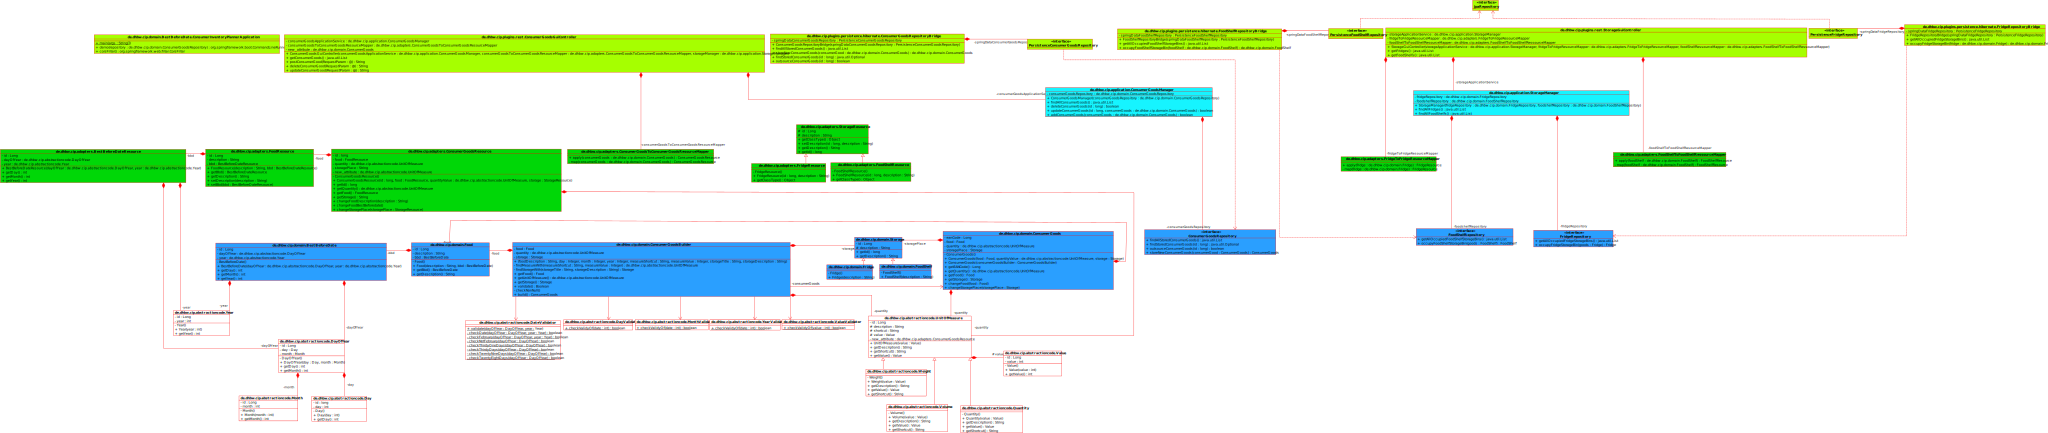
\includegraphics[width=1.0\textwidth]{Bilder/class diagram.pdf}
%	\caption[UML-Diagramm des Software-Entwurfs.]{Das UML-Diagramm des Software-Entwurfs mit entsprechend der \textit{Clean Architecture} farblich kategorisierten Klassen.}
%	\label{fig:uml-diagramm}
%\end{figure}

Die Software dient als \ac{REST}-Server zur Verwaltung der Lebensmittel Zuhause.
Dabei können Lebensmittel sowohl im Kühlschrank, der Gefriertruhe oder in einem Regal gelagert werden.
Neue Lebensmittel können angelegt werden.
Dabei ist die Bezeichnung des Lebensmitttels sowie die entsprechende Menge und das Mindesthaltbarkeitsdatum relevant.
Bei fehlerhafter Eingabe oder dem teilweisen Verbrauch können entsprechende Werte angepasst werden.
Verbrauchte Lebensmittel können gelöscht werden.
Dementsprechend sieht eine Umsetzung der einzelnen Schichten wie folgt aus:

\subsection*{\textit{Abstraction Code}-Schicht}
In der \href{https://github.com/lucasmerkel/dhbw-advancedswe-programmentwurf/tree/main/swe_programmentwurf/consumergoods-inventory-planner/4-cip-abstractioncode}{\code{Abstraction Code}}-Schicht befinden sich Klassen für die Verwaltung der Maßeinheit der Lebensmittel.
Die Klasse \href{https://github.com/lucasmerkel/dhbw-advancedswe-programmentwurf/blob/d5c89113d12c3b877ddc4d6a99225b277ddd468f/swe_programmentwurf/consumergoods-inventory-planner/4-cip-abstractioncode/src/main/java/de/dhbw/cip/abstractioncode/UnitOfMeasure.java}{\code{UnitOfMeasure}} ist die Superklasse der Subklassen \href{https://github.com/lucasmerkel/dhbw-advancedswe-programmentwurf/blob/d5c89113d12c3b877ddc4d6a99225b277ddd468f/swe_programmentwurf/consumergoods-inventory-planner/4-cip-abstractioncode/src/main/java/de/dhbw/cip/abstractioncode/Quantity.java}{\code{Quantity}}, \href{https://github.com/lucasmerkel/dhbw-advancedswe-programmentwurf/blob/d5c89113d12c3b877ddc4d6a99225b277ddd468f/swe_programmentwurf/consumergoods-inventory-planner/4-cip-abstractioncode/src/main/java/de/dhbw/cip/abstractioncode/Volume.java}{\code{Volume}} sowie \href{https://github.com/lucasmerkel/dhbw-advancedswe-programmentwurf/blob/d5c89113d12c3b877ddc4d6a99225b277ddd468f/swe_programmentwurf/consumergoods-inventory-planner/4-cip-abstractioncode/src/main/java/de/dhbw/cip/abstractioncode/Weight.java}{\code{Weight}}.
Diese Klassen repräsentieren die zugehörige Maßeinheit. Der entsprechende Wert wird durch eine Referenz auf ein Objekt der Klasse \href{https://github.com/lucasmerkel/dhbw-advancedswe-programmentwurf/blob/d5c89113d12c3b877ddc4d6a99225b277ddd468f/swe_programmentwurf/consumergoods-inventory-planner/4-cip-abstractioncode/src/main/java/de/dhbw/cip/abstractioncode/Value.java}{\code{Value}} gespeichert.
Gleiches gilt für die Repräsentation des Datums eines Tages, Monats und Jahres.
Dafür dienen die Klassen \href{https://github.com/lucasmerkel/dhbw-advancedswe-programmentwurf/blob/d5c89113d12c3b877ddc4d6a99225b277ddd468f/swe_programmentwurf/consumergoods-inventory-planner/4-cip-abstractioncode/src/main/java/de/dhbw/cip/abstractioncode/Day.java}{\code{Day}}, \href{https://github.com/lucasmerkel/dhbw-advancedswe-programmentwurf/blob/d5c89113d12c3b877ddc4d6a99225b277ddd468f/swe_programmentwurf/consumergoods-inventory-planner/4-cip-abstractioncode/src/main/java/de/dhbw/cip/abstractioncode/Month.java}{\code{Month}} sowie \href{https://github.com/lucasmerkel/dhbw-advancedswe-programmentwurf/blob/d5c89113d12c3b877ddc4d6a99225b277ddd468f/swe_programmentwurf/consumergoods-inventory-planner/4-cip-abstractioncode/src/main/java/de/dhbw/cip/abstractioncode/Year.java}{\code{Year}}.
Die Klassen für die Maßeinheit und die Repräsentation eines Tages, eines Monats sowie eines Jahres sind in dieser Schicht festgelegt, da die Informationsrepräsentation der Klassen auf domänenübergreifendes Wissen zurückzuführen ist, dessen Änderung und somit auch das der Klassen ausgeschlossen.
Die Klassen benötigen zudem keine Abhängigkeit zu Klassen der äußeren Schichten.

\subsection*{\textit{Domain Code}-Schicht}
Die \href{https://github.com/lucasmerkel/dhbw-advancedswe-programmentwurf/tree/main/swe_programmentwurf/consumergoods-inventory-planner/3-cip-domain}{\code{Domain Code}}-Schicht enthält die für den Anwendungsfall der Software relevanten Domänen.
Dazu zählt zum einen die Klasse \href{https://github.com/lucasmerkel/dhbw-advancedswe-programmentwurf/blob/main/swe_programmentwurf/consumergoods-inventory-planner/3-cip-domain/src/main/java/de/dhbw/cip/domain/ConsumerGoods.java}{\code{ConsumerGoods}}.
Diese Klasse dient der Repräsentation der Lebensmittel als einer der Domänen.
Innerhalb der Klasse \href{}{\code{ConsumerGoods}} werden dabei die weiteren Klassen \href{https://github.com/lucasmerkel/dhbw-advancedswe-programmentwurf/blob/d5c89113d12c3b877ddc4d6a99225b277ddd468f/swe_programmentwurf/consumergoods-inventory-planner/3-cip-domain/src/main/java/de/dhbw/cip/domain/Food.java}{\code{Food}} als eigentliches Lebensmittel, \href{https://github.com/lucasmerkel/dhbw-advancedswe-programmentwurf/blob/d5c89113d12c3b877ddc4d6a99225b277ddd468f/swe_programmentwurf/consumergoods-inventory-planner/3-cip-domain/src/main/java/de/dhbw/cip/domain/UnitOfMeasure.java}{\code{UnitOfMeasure}} als Klasse für die Maßeinheit sowie \href{https://github.com/lucasmerkel/dhbw-advancedswe-programmentwurf/blob/d5c89113d12c3b877ddc4d6a99225b277ddd468f/swe_programmentwurf/consumergoods-inventory-planner/3-cip-domain/src/main/java/de/dhbw/cip/domain/Storage.java}{\code{Storage}} als Klasse für den Lagerort verwaltet.
Die Klasse \href{}{\code{UnitOfMeasure}} ist wie bereits erläutert Teil der \textit{Abstraction Code}-Schicht und somit ist die Abhängigkeit möglich.
Die Klasse \href{}{\code{Storage}} ist die Superklasse für die Lagerortsklassen \href{https://github.com/lucasmerkel/dhbw-advancedswe-programmentwurf/blob/d5c89113d12c3b877ddc4d6a99225b277ddd468f/swe_programmentwurf/consumergoods-inventory-planner/3-cip-domain/src/main/java/de/dhbw/cip/domain/Fridge.java}{\code{Fridge}} sowie \href{https://github.com/lucasmerkel/dhbw-advancedswe-programmentwurf/blob/d5c89113d12c3b877ddc4d6a99225b277ddd468f/swe_programmentwurf/consumergoods-inventory-planner/3-cip-domain/src/main/java/de/dhbw/cip/domain/FoodShelf.java}{\code{FoodShelf}} und speichern die Beschreibung des Lagerorts.
Eine weitere Klasse ist \href{}{\code{Food}}. Diese Klasse repräsentiert die Bezeichnung des zu speichernden Lebensmittels sowie das dazugehörige Mindesthaltbarkeitsdatum.
Das Mindesthaltbarkeitsdatum wird in der Klasse \href{https://github.com/lucasmerkel/dhbw-advancedswe-programmentwurf/blob/d5c89113d12c3b877ddc4d6a99225b277ddd468f/swe_programmentwurf/consumergoods-inventory-planner/3-cip-domain/src/main/java/de/dhbw/cip/domain/BestBeforeDate.java}{\code{BestBeforeDate}} verwaltet.

Darüber hinaus befinden sich in der \textit{Domain Code}-Schicht die Interfaces \href{https://github.com/lucasmerkel/dhbw-advancedswe-programmentwurf/blob/d5c89113d12c3b877ddc4d6a99225b277ddd468f/swe_programmentwurf/consumergoods-inventory-planner/3-cip-domain/src/main/java/de/dhbw/cip/domain/ConsumerGoodsRepository.java}{\code{ConsumerGoodsRepository}}, \href{https://github.com/lucasmerkel/dhbw-advancedswe-programmentwurf/blob/d5c89113d12c3b877ddc4d6a99225b277ddd468f/swe_programmentwurf/consumergoods-inventory-planner/3-cip-domain/src/main/java/de/dhbw/cip/domain/FridgeRepository.java}{\code{FridgeRepository}} und \href{https://github.com/lucasmerkel/dhbw-advancedswe-programmentwurf/blob/d5c89113d12c3b877ddc4d6a99225b277ddd468f/swe_programmentwurf/consumergoods-inventory-planner/3-cip-domain/src/main/java/de/dhbw/cip/domain/FoodShelfRepository.java}{\code{FoodShelfRepository}}.
Diese Interfaces dienen im folgenden Verlauf der Anwendung einer \textit{Dependency Inversion}.
Die Interfaces beinhalten die abstrakten Methoden zum Finden gezielter oder aller jeweiligen Entitäten sowie dem Löschen und Hinzufügen.

Die Klassen \href{https://github.com/lucasmerkel/dhbw-advancedswe-programmentwurf/blob/d5c89113d12c3b877ddc4d6a99225b277ddd468f/swe_programmentwurf/consumergoods-inventory-planner/3-cip-domain/src/main/java/de/dhbw/cip/domain/DateValidator.java}{\code{DayValidator}}, \href{https://github.com/lucasmerkel/dhbw-advancedswe-programmentwurf/blob/d5c89113d12c3b877ddc4d6a99225b277ddd468f/swe_programmentwurf/consumergoods-inventory-planner/3-cip-domain/src/main/java/de/dhbw/cip/domain/DateValidator.java}{\code{MonthValidator}}, \href{https://github.com/lucasmerkel/dhbw-advancedswe-programmentwurf/blob/d5c89113d12c3b877ddc4d6a99225b277ddd468f/swe_programmentwurf/consumergoods-inventory-planner/3-cip-domain/src/main/java/de/dhbw/cip/domain/DateValidator.java}{\code{YearValidator}} und \href{https://github.com/lucasmerkel/dhbw-advancedswe-programmentwurf/blob/d5c89113d12c3b877ddc4d6a99225b277ddd468f/swe_programmentwurf/consumergoods-inventory-planner/3-cip-domain/src/main/java/de/dhbw/cip/domain/DateValidator.java}{\code{ValueValidator}}.
Diese Klassen dienen der Validierung der Werte für das Tagdatum, Monatsdatum, Jahresdatum und den Wert für die Menge.
Die Validierung liegt hierbei nur auf den grundlegenden Kriterien.
Dazu zählt, dass die jeweiligen Werte nicht negativ sein dürfen sowie der Wert für ein Tagdatum größer als 31 beziehungsweise das Monatsdatum über 12 ungültig ist.
Für die der Gültigkeit des Mindesthaltbarkeitsdatums als ein grundsätzlich gültiges Datum dient die Klasse \href{https://github.com/lucasmerkel/dhbw-advancedswe-programmentwurf/blob/d5c89113d12c3b877ddc4d6a99225b277ddd468f/swe_programmentwurf/consumergoods-inventory-planner/3-cip-domain/src/main/java/de/dhbw/cip/domain/DateValidator.java}{\code{DateValidator}}.

\subsection*{\textit{Application Code}-Schicht}
Eine weitere Schicht ist die \href{https://github.com/lucasmerkel/dhbw-advancedswe-programmentwurf/tree/main/swe_programmentwurf/consumergoods-inventory-planner/2-cip-application}{\code{Application Code}}-Schicht.
Darin befinden sich die Klassen \href{https://github.com/lucasmerkel/dhbw-advancedswe-programmentwurf/blob/d5c89113d12c3b877ddc4d6a99225b277ddd468f/swe_programmentwurf/consumergoods-inventory-planner/2-cip-application/src/main/java/de/dhbw/cip/application/ConsumerGoodsManager.java}{\code{ConsumerGoodsManager}} sowie \href{https://github.com/lucasmerkel/dhbw-advancedswe-programmentwurf/blob/d5c89113d12c3b877ddc4d6a99225b277ddd468f/swe_programmentwurf/consumergoods-inventory-planner/2-cip-application/src/main/java/de/dhbw/cip/application/StorageManager.java}{\code{StorageManager}}.
In diesen Klassen findet die Applikationslogik statt.
Innerhalb der Klasse \href{}{\code{ConsumerGoodsManager}} bedeutet das konkret, das Anlegen neuer \href{}{\code{ConsumerGoods}}-Objekten, das Ausgeben aller aktuell gespeicherter \href{}{\code{ConsumerGoods}}-Objekten, Verändern eines \href{}{\code{ConsumerGoods}}-Objekts sowie das Löschen von \href{}{\code{ConsumerGoods}}-Objekten.

Die Klasse \href{https://github.com/lucasmerkel/dhbw-advancedswe-programmentwurf/blob/d5c89113d12c3b877ddc4d6a99225b277ddd468f/swe_programmentwurf/consumergoods-inventory-planner/0-cip-plugins/src/main/java/de/dhbw/cip/plugins/persistence/hibernate/ConsumerGoodsRepositoryBridge.java}{\code{ConsumerGoodsRepositoryBridge}} aus der \textit{Plugin}-Schicht fungiert als Repository-Klasse für die \href{}{\code{ConsumerGoods}}-Objekte. Die beiden Klassen haben das Interface \href{}{\code{ConsumerGoodsRepository}} implementiert.
Zum Ausführen der Applikationslogik eine Abhängigkeit in eine äußere Schicht nötig. 
Um dies zu umgehen, wird als Übergabeparameter des Konstruktors ein Objekt, welches das Interface \href{}{\code{ConsumerGoodsRepository}} implementiert hat, übergeben.
Somit ist zur Kompilierungszeit keine Abhängigkeit vorhanden und ein Verwenden der äußeren Klasse zur Laufzeit möglich.
Durch das Anwenden der \href{https://github.com/lucasmerkel/dhbw-advancedswe-programmentwurf/blob/2bab7b1c200507e4550ce7025485261d0e95ce07/swe_programmentwurf/consumergoods-inventory-planner/2-cip-application/src/main/java/de/dhbw/cip/application/ConsumerGoodsManager.java#L18}{\code{Dependency Injection}} in der Klasse \textit{ConsumerGoodsManager} kann daraus eine \textit{Dependency Inversion} angewandt werden, die das Problem der Abhängigkeit zur Kompilierungszeit in eine äußere Schicht löst.
Sollte nun die Klasse \href{}{\code{ConsumerGoodsRepositoryBridge}} in der \textit{Plugin}-Schicht aufgrund eines Technologiewechsel verändert werden, kann bei Implementierung des Interfaces \href{}{\code{ConsumerGoodsRepository}} unberührt weiterverwendet werden.

Die Klasse \href{}{\code{StorageManager}} hat die gleiche Applikationslogik wie die Klasse \href{}{\code{ConsumerGoodsManager}}, jedoch mit dem Unterschied, dass es sich auf \href{}{\code{Fridge}}-Objekte sowie \href{}{\code{FoodShelf}}-Objekte bezieht.
Analog hier ist ebenfalls ein Anlegen, Ausgeben, Verändern und Löschen eines \href{}{\code{Fridge}}-Objekte oder \href{}{\code{FoodShelf}}-Objektes möglich.

Auch in der Klasse \href{}{\code{StorageManager}} findet eine \href{https://github.com/lucasmerkel/dhbw-advancedswe-programmentwurf/blob/2bab7b1c200507e4550ce7025485261d0e95ce07/swe_programmentwurf/consumergoods-inventory-planner/2-cip-application/src/main/java/de/dhbw/cip/application/StorageManager.java#L21}{\code{Dependency Inversion}} für die Klassen der Repositories für die einzelnen Storage-Ausprägungen statt.
Die Klassen \href{}{\code{FridgeRepositoryBridge}} und \href{}{\code{FoodShelfRepositoryBridge}} dienen als Repository-Klassen für die jeweiligen \href{}{\code{Fridge}}-Objekte und \href{}{\code{FoodShelf}}-Objekte. Die beiden Klassen haben das Interface \href{}{\code{FridgeRepository}} beziehungsweise \href{}{\code{FoodShelfRepository}} implementiert.
Auch hier wäre zum Ausführen der Applikationslogik eine Abhängigkeit in eine äußere Schicht nötig. Um dies zu umgehen, wird auch hierbei als Übergabeparameter des Konstruktors ein Objekt, welches das Interface \href{}{\code{FridgeRepository}} beziehungsweise \href{}{\code{FoodShelfRepository}} implementiert hat, übergeben.
Somit ist zur Kompilierungszeit keine Abhängigkeit vorhanden und ein Verwenden der äußeren Klasse möglich.

%\todo[]{eventuell RenderModell umsetzen, auch in Richtung des ApplicationCodes}

\subsection*{\textit{Adapters}-Schicht}
Eine weitere Schicht ist die \href{https://github.com/lucasmerkel/dhbw-advancedswe-programmentwurf/tree/main/swe_programmentwurf/consumergoods-inventory-planner/1-cip-adapters}{\code{Adapters}}-Schicht.
Diese Schicht dient als \textit{Anti Corruption Layer}, indem sie die inneren Schichten von den äußeren Schichten trennt.
Dementsprechend sind die Domänen-Klassen aus der \textit{Domain}-Schicht, die zur Kommunikation mit den äußeren Schichten benötigt werden, in dieser Schicht repliziert.
Dazu zählen die in Tabelle \ref{clean-architecture>klassen-adapters} mit den in der \textit{Domain}-Schicht gegenübergestellten Klassen:

\begin{table}[H]
    \centering
\begin{tabular}[h]{|c|c|}
	\hline
	\textbf{Domain-Schicht} & \textbf{Adapters-Schicht} \\
	\hline
	ConsumerGoods & ConsumerGoodsResource \\
	\hline
	Food & FoodResource \\
	\hline
	BestBeforeDate & BestBeforeDateResource \\
	\hline
	Food & FoodResource \\
	\hline
	Storage & StorageResource \\
	\hline
	Fridge & FridgeResource \\
	\hline
	FoodShelf & FoodShelfResource \\
    \hline
\end{tabular}
    \caption{Gegenüberstellung der in der \textit{Adapters}-Schicht abgebildeten Klassen aus der \textit{Domain}-Schicht.}
    \label{clean-architecture>klassen-adapters}
\end{table}

Durchgeführt wird diese Trennung der inneren und äußeren Schichten durch die Klassen \href{https://github.com/lucasmerkel/dhbw-advancedswe-programmentwurf/blob/d5c89113d12c3b877ddc4d6a99225b277ddd468f/swe_programmentwurf/consumergoods-inventory-planner/1-cip-adapters/src/main/java/de/dhbw/cip/adapters/ConsumerGoodsToConsumerGoodsResourceMapper.java}{\code{ConsumerGoodsToConsumerGoodsRessourceMapper}}, \href{https://github.com/lucasmerkel/dhbw-advancedswe-programmentwurf/blob/d5c89113d12c3b877ddc4d6a99225b277ddd468f/swe_programmentwurf/consumergoods-inventory-planner/1-cip-adapters/src/main/java/de/dhbw/cip/adapters/FridgeToFridgeResourceMapper.java}{\code{FridgeToFridgeRessourceMapper}} sowie \href{https://github.com/lucasmerkel/dhbw-advancedswe-programmentwurf/blob/d5c89113d12c3b877ddc4d6a99225b277ddd468f/swe_programmentwurf/consumergoods-inventory-planner/1-cip-adapters/src/main/java/de/dhbw/cip/adapters/FoodShelfToFoodShelfRessourceMapper.java}{\code{FoodShelfToFoodShelfMapper}}.
Die Erstellung neuer Resource-Objekte beruht auf den Daten der Domänen-Objekte.
Die dadurch erzeugten Resource-Objekte können nun von Objekten der Klassen in der \textit{Plugin}-Schicht verwendet werden.

\subsection*{\textit{Plugin}-Schicht}
Die äußerste Schicht bildet die \href{https://github.com/lucasmerkel/dhbw-advancedswe-programmentwurf/tree/main/swe_programmentwurf/consumergoods-inventory-planner/0-cip-plugins}{\code{Plugin}}-Schicht.

\subsubsection*{Main}
Zum einen enthält die Plugin-Schicht die Main-Methode zum Starten des Projekts.
Aufgrund der Tatsache, dass die Main-Methode technisch bedingt und somit keinerlei Bezug zur Anwendung und deren Geschäftsprozesse hat, ist sie in der äußersten Schicht anzusetzen.
Dementsprechend befindet sich die Main-Methode in der Klasse \href{https://github.com/lucasmerkel/dhbw-advancedswe-programmentwurf/blob/d5c89113d12c3b877ddc4d6a99225b277ddd468f/swe_programmentwurf/consumergoods-inventory-planner/0-cip-plugins/src/main/java/de/dhbw/cip/ConsumerInventoryPlannerApplication.java}{\code{ConsumerInventoryPlannerApplication}}, die sich im Package \href{https://github.com/lucasmerkel/dhbw-advancedswe-programmentwurf/tree/main/swe_programmentwurf/consumergoods-inventory-planner/0-cip-plugins/src/main/java/de/dhbw/cip}{\code{de.dhbw.cip.main}} befindet.

\subsubsection*{JPA}
Daneben gibt es in der \textit{Plugin}-Schicht das Package \href{https://github.com/lucasmerkel/dhbw-advancedswe-programmentwurf/tree/main/swe_programmentwurf/consumergoods-inventory-planner/0-cip-plugins/src/main/java/de/dhbw/cip/plugins/persistence/hibernate}{\code{de.dhbw.cip.plugins.persistence.hibernate}}.
Es enthält die Klassen \href{https://github.com/lucasmerkel/dhbw-advancedswe-programmentwurf/blob/d5c89113d12c3b877ddc4d6a99225b277ddd468f/swe_programmentwurf/consumergoods-inventory-planner/0-cip-plugins/src/main/java/de/dhbw/cip/plugins/persistence/hibernate/ConsumerGoodsRepositoryBridge.java}{\code{ConsumerGoodsRepositoryBridge}}, \href{https://github.com/lucasmerkel/dhbw-advancedswe-programmentwurf/blob/d5c89113d12c3b877ddc4d6a99225b277ddd468f/swe_programmentwurf/consumergoods-inventory-planner/0-cip-plugins/src/main/java/de/dhbw/cip/plugins/persistence/hibernate/FridgeRepositoryBridge.java}{\code{FridgeRepositoryBridge}} sowie \href{https://github.com/lucasmerkel/dhbw-advancedswe-programmentwurf/blob/d5c89113d12c3b877ddc4d6a99225b277ddd468f/swe_programmentwurf/consumergoods-inventory-planner/0-cip-plugins/src/main/java/de/dhbw/cip/plugins/persistence/hibernate/FoodShelfRepositoryBridge.java}{\code{FoodShelfRepositoryBridge}}.
Diese Klassen dienen als Repository-Klassen für die Objekte der jeweiligen Klassen \href{}{\code{ConsumerGoods}}, \href{}{\code{Fridge}} sowie \href{}{\code{FoodShelf}}.
Die Klassen haben jeweils das aus der \textit{Domain}-Schicht dazugehörige Interface implementiert.
Die Bridge dient dabei als Bindeglied zwischen dem internen Repository sowie der durch das Spring Framework bereitgestellten Oberklasse \href{}{\code{JpaRepository}}, welche für die spätere Anbindung an eine Datenbank zur Persistierung benötigt wird.
Dadurch kann eine Trennung zwischen der Geschäftslogik und der Persistierung durch das Spring Framework durchgeführt werden.
Die Bridge entspricht zudem einem Entwurfsmuster und wird im Kapitel \ref{entwurfsmuster} ebenfalls analysiert.
Des Weiteren sind in dem Package die Klassen \href{https://github.com/lucasmerkel/dhbw-advancedswe-programmentwurf/blob/d5c89113d12c3b877ddc4d6a99225b277ddd468f/swe_programmentwurf/consumergoods-inventory-planner/0-cip-plugins/src/main/java/de/dhbw/cip/plugins/persistence/hibernate/PersistenceConsumerGoodsRepository.java}{\code{PersistenceConsumerGoodsRepository}}, \href{https://github.com/lucasmerkel/dhbw-advancedswe-programmentwurf/blob/d5c89113d12c3b877ddc4d6a99225b277ddd468f/swe_programmentwurf/consumergoods-inventory-planner/0-cip-plugins/src/main/java/de/dhbw/cip/plugins/persistence/hibernate/PersistenceFridgeRepository.java}{\code{PersistenceFridgeRepository}} sowie \href{https://github.com/lucasmerkel/dhbw-advancedswe-programmentwurf/blob/d5c89113d12c3b877ddc4d6a99225b277ddd468f/swe_programmentwurf/consumergoods-inventory-planner/0-cip-plugins/src/main/java/de/dhbw/cip/plugins/persistence/hibernate/PersistenceFoodShelfRepository.java}{\code{PersistenceFoodShelfRepository}} enthalten.
Wie bereits erwähnt, erben diese Klassen von der Oberklasse \href{}{\code{JpaRepository}}.
Diese Klassen wird durch das Spring-Framework bereitgestellt und dient der Persistierung auf einer Datenbank.
Diese Klassen stellen somit die Möglichkeit bereit, die Anbindung an eine Datenbank zu ermöglichen.
Die Implementierung ist jedoch nicht in den Anforderungen festgelegt, weshalb ausschließlich die geforderten Grundlagen zur Umsetzung bereitgestellt sind.

\subsubsection*{REST-Controller}
Zuletzt findet sich in der \textit{Plugin}-Schicht das Package \href{https://github.com/lucasmerkel/dhbw-advancedswe-programmentwurf/tree/main/swe_programmentwurf/consumergoods-inventory-planner/0-cip-plugins/src/main/java/de/dhbw/cip/plugins/rest}{\code{de.dhbw.cip.plugins.rest}}.
Darin befinden sich die Klassen \href{https://github.com/lucasmerkel/dhbw-advancedswe-programmentwurf/blob/d5c89113d12c3b877ddc4d6a99225b277ddd468f/swe_programmentwurf/consumergoods-inventory-planner/0-cip-plugins/src/main/java/de/dhbw/cip/plugins/rest/ConsumerGoodsGuiController.java}{\code{ConsumerGoodsGuiController}} sowie \href{https://github.com/lucasmerkel/dhbw-advancedswe-programmentwurf/blob/d5c89113d12c3b877ddc4d6a99225b277ddd468f/swe_programmentwurf/consumergoods-inventory-planner/0-cip-plugins/src/main/java/de/dhbw/cip/plugins/rest/StorageGuiController.java}{\code{StorageGuiController}}.
Bei diesen Klassen handelt es sich um den \ac{REST}-Controller zur Interaktion über das HTTP-Protokoll mit der \ac{GUI}.
Die GUI ist mit der Technologie \textit{Angular} erstellt worden.
Sie dient lediglich der Repräsentation der Funktionalität des \ac{REST}-Services und wird daher innerhalb des Softwareentwurfs nicht tiefer analysiert.
Der \ac{REST}-Controller dient somit als Schnittstelle zur \ac{GUI} und befindet sich daher in der \textit{Plugin}-Schicht.
Zum Erhalt der darzustellenden Daten werden Instanzen des jeweiligen Application Services sowie des Resource Mappers als Übergabeparemeter des Konstruktors übergeben.
Dadurch können zum Senden der Entitäten die in der \textit{Adapter}-Schicht erzeugten Resource-Entitäten gestreamt und als Liste gesendet werden.
Gleichzeitig können über eine Abhängkeit zum entsprechenden Application Service Entitäten entsprechend der über die \ac{GUI} übermittelnden Daten erzeugt, verändert oder gelöscht werden.
Die Code-Ausschnitte verdeutlichen die Interaktionen des \ac{REST}-Controllers am Beispiel der Klasse \textit{ConsumerGoodsGuiController}.

\subsubsection*{Testklassen}
In der Plugin-Schicht befinden sich ebenfalls die Klassen \href{https://github.com/lucasmerkel/dhbw-advancedswe-programmentwurf/blob/d5c89113d12c3b877ddc4d6a99225b277ddd468f/swe_programmentwurf/consumergoods-inventory-planner/0-cip-plugins/src/test/java/de/dhbw/cip/AddConsumerGoodsTest.java}{\code{AddConsumerGoodsTest}}, 
\href{https://github.com/lucasmerkel/dhbw-advancedswe-programmentwurf/blob/d5c89113d12c3b877ddc4d6a99225b277ddd468f/swe_programmentwurf/consumergoods-inventory-planner/0-cip-plugins/src/test/java/de/dhbw/cip/DateValidatorTest.java}{\code{DateValidatorTest}} 
\href{https://github.com/lucasmerkel/dhbw-advancedswe-programmentwurf/blob/d5c89113d12c3b877ddc4d6a99225b277ddd468f/swe_programmentwurf/consumergoods-inventory-planner/0-cip-plugins/src/test/java/de/dhbw/cip/DayDateTest.java}{\code{DayDateTest}} 
\href{https://github.com/lucasmerkel/dhbw-advancedswe-programmentwurf/blob/d5c89113d12c3b877ddc4d6a99225b277ddd468f/swe_programmentwurf/consumergoods-inventory-planner/0-cip-plugins/src/test/java/de/dhbw/cip/MonthDateTest.java}{\code{MonthDateTest}}
\href{https://github.com/lucasmerkel/dhbw-advancedswe-programmentwurf/blob/d5c89113d12c3b877ddc4d6a99225b277ddd468f/swe_programmentwurf/consumergoods-inventory-planner/0-cip-plugins/src/test/java/de/dhbw/cip/RestTest.java}{\code{RestTest}}
\href{https://github.com/lucasmerkel/dhbw-advancedswe-programmentwurf/blob/d5c89113d12c3b877ddc4d6a99225b277ddd468f/swe_programmentwurf/consumergoods-inventory-planner/0-cip-plugins/src/test/java/de/dhbw/cip/UnitOfMeasureValueTest.java}{\code{UnitOfMeasureValueTest}}
\href{https://github.com/lucasmerkel/dhbw-advancedswe-programmentwurf/blob/d5c89113d12c3b877ddc4d6a99225b277ddd468f/swe_programmentwurf/consumergoods-inventory-planner/0-cip-plugins/src/test/java/de/dhbw/cip/UpdateConsumerGoodsTest.java}{\code{UpdateConsumerGoodsTest}} und 
\href{https://github.com/lucasmerkel/dhbw-advancedswe-programmentwurf/blob/d5c89113d12c3b877ddc4d6a99225b277ddd468f/swe_programmentwurf/consumergoods-inventory-planner/0-cip-plugins/src/test/java/de/dhbw/cip/YearDateTest.java}{\code{YearDateTest}}.
Diese Klassen dienen für Unit-Tests und werden im Kapitel \ref{unit-tests} ausführlicher beschrieben.

\subsection*{Frameworks}
Während die Verwendung von Bibliotheken Funktionalitäten einer Klasse innerhalb einer Schicht erweitern, versuchen Frameworks Einfluss auf die gesammte Struktur und somit auch schichtübergreifend zu nehmen.
Neben der Wahl der Programmiersprache ist das eine weitere grundlegende Entscheidung, die zu Beginn getroffen wird und zu grundlegenden Abhängigkeiten der Software führen kann.
Der Nachteil ist, dass die Entwicklung des Frameworks nicht beeinflusst werden kann.
Somit können Weiterentwicklungen nicht mehr mit der Konzeption des Softwareentwurfs übereinstimmen und das hätte zur große Wirkungen in Form von Änderungen oder einer Neuentwicklung zur Folge.
Deshalb wird die Wahl eines Frameworks als grundlegende Abhängigkeit gesehen und sollte bedacht gewählt werden.
Es bietet sich an, soweit das Framework dies zulässt, die Funktionalitäten bestenfalls an die \textit{Plugin}-Schicht zu drängen.

Bei diesem Softwareentwurf wurde das Framework SpringBoot gewählt.
SpringBoot vereinfacht die Anwendung von Webanwendeungen, wie in diesem Softwareentwurf in Form eines Webservices.
Das Framework stellt nötige Webserver bereit und vereinfacht die Anbindung mit Frameworks zur Persistierung wie beispielsweise Hibernate.
Das unterstützt bei der Entwicklung eines Webservices.

\subsubsection*{Strukturierung}
Ein Vorteil ist die Struktur, die SpringBoot vorgibt.
Dadurch kann es bei der Umsetzung der definierten Schichten der \textit{Clean Architecture} für die Controller-Klassen und Service-Klassen unterstützen.
Es findet jedoch durch die Annotation des Frameworks zugleich eine Abhängigkeit ab.
Beispiele sind die Kennzeichnung des Controllers mittels \textit{@RestController} in der Klasse \href{https://github.com/lucasmerkel/dhbw-advancedswe-programmentwurf/blob/d5c89113d12c3b877ddc4d6a99225b277ddd468f/swe_programmentwurf/consumergoods-inventory-planner/0-cip-plugins/src/main/java/de/dhbw/cip/plugins/rest/ConsumerGoodsGuiController.java#L38}{\code{ConsumerGoodsGuiController}} und \href{https://github.com/lucasmerkel/dhbw-advancedswe-programmentwurf/blob/d5c89113d12c3b877ddc4d6a99225b277ddd468f/swe_programmentwurf/consumergoods-inventory-planner/0-cip-plugins/src/main/java/de/dhbw/cip/plugins/rest/StorageGuiController.java#L17}{\code{StorageGuiController}} sowie die Kennzeichnung einer Service-Klasse mit der \textit{@Service} Annotation in den Klassen \href{https://github.com/lucasmerkel/dhbw-advancedswe-programmentwurf/blob/d5c89113d12c3b877ddc4d6a99225b277ddd468f/swe_programmentwurf/consumergoods-inventory-planner/2-cip-application/src/main/java/de/dhbw/cip/application/ConsumerGoodsManager.java#L12}{\code{ConsumerGoodsManager}} und \href{https://github.com/lucasmerkel/dhbw-advancedswe-programmentwurf/blob/d5c89113d12c3b877ddc4d6a99225b277ddd468f/swe_programmentwurf/consumergoods-inventory-planner/2-cip-application/src/main/java/de/dhbw/cip/application/StorageManager.java#L14}{\code{StroageManager}}.
%Convention over Configuration => KISS und Don't repeat yourself

\subsubsection*{Dependency Injection durch Inversion of Control}
Ein weiterer Vorteil von Spring Boot ist der Spring Inversion of Control Container. Der Inversion of Control Container verwaltet zur Laufzeit die erzeugten Beans und ermöglicht sehr einfach Dependency Injection, indem der Container die Zuweisung übernimmt, wie es beispielsweise in den Klassen \href{https://github.com/lucasmerkel/dhbw-advancedswe-programmentwurf/blob/d5c89113d12c3b877ddc4d6a99225b277ddd468f/swe_programmentwurf/consumergoods-inventory-planner/2-cip-application/src/main/java/de/dhbw/cip/application/ConsumerGoodsManager.java#L18}{\code{ConsumerGoodsManager}} oder \href{https://github.com/lucasmerkel/dhbw-advancedswe-programmentwurf/blob/d5c89113d12c3b877ddc4d6a99225b277ddd468f/swe_programmentwurf/consumergoods-inventory-planner/0-cip-plugins/src/main/java/de/dhbw/cip/plugins/rest/ConsumerGoodsGuiController.java#L47}{\code{ConsumerGoodsGuiController}} der Fall ist.

Auch hierbei ist zu beachten, dass durch die nötige Annotation \textit{@Autowired} des Frameworks eine gewisse Abhängigkeit stattfindet, wie es beispielsweise in den Klassen \href{https://github.com/lucasmerkel/dhbw-advancedswe-programmentwurf/blob/d5c89113d12c3b877ddc4d6a99225b277ddd468f/swe_programmentwurf/consumergoods-inventory-planner/2-cip-application/src/main/java/de/dhbw/cip/application/ConsumerGoodsManager.java#L17}{\code{ConsumerGoodsManager}} oder \href{https://github.com/lucasmerkel/dhbw-advancedswe-programmentwurf/blob/d5c89113d12c3b877ddc4d6a99225b277ddd468f/swe_programmentwurf/consumergoods-inventory-planner/0-cip-plugins/src/main/java/de/dhbw/cip/plugins/rest/ConsumerGoodsGuiController.java#L46}{\code{ConsumerGoodsGuiController}} der Fall ist.

\subsubsection*{Persistierung}
Eine weitere Unterstützung bietet Spring Boot bei der Persistierung.
Hierbei wurde die Persistierung jedoch mithilfe des \textit{Bridge}-Entwurfmusters, wie in Kapitel \ref{entwurfsmuster} genauer erläutert, in die Plugin-Schicht gedrängt.
Beispielklassen ConsumerGoodsBridge und PersistenceConsumerGoodsRepository

Jedoch befinden sich die nötigen Annotationen in der Domäne, was sehr abhängig ist und im Gegensatz zu den bereits erwähnten Annotationen gewissermaßen stärker in das Gewicht fällt, weil es sich hierbei um die Domänenklassen handelt und diese unabhängig von verwendeten Technologien sein sollten.
Ein nichtauszuschließender Technologiewechsel führt somit zu einer Anpassung der Klassen in der \textit{Domain}-Schicht, was die Umsetzung der \textit{Clean Architecture} verletzt.
Als Beispiel zählen die nötigen Annotierungen die Kennzeichnung als Entität, zur späteren Bezeichnung von Tabellen, in denen die Attributwerte persistiert werden oder nötige Metainformationen wie beispielsweise die Zuweisung der Funktion eines Attributs als Id. Ein Beispiel sind die Annotationen \href{https://github.com/lucasmerkel/dhbw-advancedswe-programmentwurf/blob/d5c89113d12c3b877ddc4d6a99225b277ddd468f/swe_programmentwurf/consumergoods-inventory-planner/3-cip-domain/src/main/java/de/dhbw/cip/domain/ConsumerGoods.java#L16}{\textit{@Entity}}, \href{https://github.com/lucasmerkel/dhbw-advancedswe-programmentwurf/blob/d5c89113d12c3b877ddc4d6a99225b277ddd468f/swe_programmentwurf/consumergoods-inventory-planner/3-cip-domain/src/main/java/de/dhbw/cip/domain/ConsumerGoods.java#L20}{\textit{@Id}}, \href{https://github.com/lucasmerkel/dhbw-advancedswe-programmentwurf/blob/d5c89113d12c3b877ddc4d6a99225b277ddd468f/swe_programmentwurf/consumergoods-inventory-planner/3-cip-domain/src/main/java/de/dhbw/cip/domain/ConsumerGoods.java#L21}{\textit{@Column}} und \href{https://github.com/lucasmerkel/dhbw-advancedswe-programmentwurf/blob/d5c89113d12c3b877ddc4d6a99225b277ddd468f/swe_programmentwurf/consumergoods-inventory-planner/3-cip-domain/src/main/java/de/dhbw/cip/domain/ConsumerGoods.java#L24}{\textit{@OneToOne}} in der Klasse \href{https://github.com/lucasmerkel/dhbw-advancedswe-programmentwurf/blob/d5c89113d12c3b877ddc4d6a99225b277ddd468f/swe_programmentwurf/consumergoods-inventory-planner/3-cip-domain/src/main/java/de/dhbw/cip/domain/ConsumerGoods.java}{\code{ConsumerGoods}}.

Ein weiterer Nachteil ist, dass zur Persistierung Attributtypen eindeutig zuweisbar sein müssen.
Das bedeutet, dass Attribute, die mit einem Interface als Typ deklariert werden, nicht möglich sind.
Stattdessen muss eine Deklarierung einer konkreten Klasse oder Superklasse erfolgen.
Ein Beispiel ist die Deklaration zur Zuweisung der \href{https://github.com/lucasmerkel/dhbw-advancedswe-programmentwurf/blob/2bab7b1c200507e4550ce7025485261d0e95ce07/swe_programmentwurf/consumergoods-inventory-planner/3-cip-domain/src/main/java/de/dhbw/cip/domain/ConsumerGoods.java#L28}{Menge} und des \href{https://github.com/lucasmerkel/dhbw-advancedswe-programmentwurf/blob/2bab7b1c200507e4550ce7025485261d0e95ce07/swe_programmentwurf/consumergoods-inventory-planner/3-cip-domain/src/main/java/de/dhbw/cip/domain/ConsumerGoods.java#L31}{Lagerplatzes} in der Klasse \href{}{\code{ConsumerGoods}} mit den Superklassen \href{https://github.com/lucasmerkel/dhbw-advancedswe-programmentwurf/blob/2bab7b1c200507e4550ce7025485261d0e95ce07/swe_programmentwurf/consumergoods-inventory-planner/4-cip-abstractioncode/src/main/java/de/dhbw/cip/abstractioncode/UnitOfMeasure.java}{\code{UnitOfMeasure}} sowie \href{https://github.com/lucasmerkel/dhbw-advancedswe-programmentwurf/blob/2bab7b1c200507e4550ce7025485261d0e95ce07/swe_programmentwurf/consumergoods-inventory-planner/3-cip-domain/src/main/java/de/dhbw/cip/domain/Storage.java}{\code{Storage}} realisiert.
Wäre diese Einschränkung für das Persistieren nicht gegeben, könnten \href{}{\code{UnitOfMeasure}} und \href{}{\code{Storage}} auch als Interface realisiert sowie das Interface \href{}{\code{StorableGood}}, dass von der Klasse \href{}{\code{Food}} daraufhin implementiert werden kann, genutzt werden.
\chapter{Programming Principles}
Im Folgenden Kapitel werden die \textit{Programming Principles} erläutert und in Bezug auf den Programmentwurf analysiert sowie Umsetzungen begründet.

\section{Zu betrachtende Programming Principles}
Programming Principles dienen als Prinzipien in der Softwareentwicklung.
Dementsprechend sind Programming Principles als allgemein anerkannte Regeln zur Begründung und Argumentation von Umsetzungen zu verstehen.
Sie entsprechen somit Grundlage für Entscheidungen und betrachten dabei das gesamte Softwareprojekt.
Die Programming Principles sind dabei eine kontextlose Idealvorstellung und haben die Funktion als Leitlinien für zielgerichtetetes Handeln.
Das hat zur Folge, dass kontextabhängig gewisse Abweichungen nötig sein können.
Daher gilt es, neben dem Anwenden der Prinzipien auch mögliche Abweichungen zu begründen.
Gleichzeitig können sich die jeweiligen Prinzipien gegeneinander widersprechen.
Hierbei ist es nötig, kontextabhängig entsprechend abzuwirken und die Entscheidung ebenfalls zu begründen.

Zu den betrachteten Programming Principles zählt SOLID.
SOLID setzt sich aus den Prinzipien
\begin{itemize}
    \item \textit{Single Responsibility Principle} (SRP),
    \item \textit{Open/Closed Principle} (OCP),
    \item \textit{Liskov Substitution Principle} (LSP),
    \item \textit{Interface Segregation Principle} (ISP),
    \item \textit{Dependency Inversion Principle} (DIP)
  \end{itemize}
zusammen.
Die SOLID-Regeln haben das Ziel, unter Anwendung der Regeln wartbare sowie erweiterbare Systeme sowie eine langlebige Codebasis zu schaffen.

Um dies zu gewährleisten, beschreibt die erste Regel, das \textit{Single Responsibility Principle}, das Prinzip der einzigen Zuständigkeit.
Die Regel besagt, dass eine Klasse nur einen zeinigen Grund haben sollte, sich zu ändern.
Eine Klasse sollte somit nur eine Verantwortlichkeit haben.
Ein Objekt der Klasse hat somit eine klar definierte Aufgabe und übergeordnetes Verhalten wird durch das Zusammenspiel mehrerer Klassen ermöglicht.
Damit soll vermieden werden, dass es zu einer Überdeckung des Sourcecodes bezogen auf dessen Anwendung für die Zuständigkeit kommt.
Dieses Problem bezeichnet man als Feature Drift.
Eine Änderung an diesem Sourcecode, der für mehrere Zuständigkeiten genutzt wird, hätte zur Folge, dass ungewollt eine anderweitige Zuständigkeit der Klasse verändert wird.
Das Problem kann auch visuell mittels eines Koordinatensystems dargestellt werden.
Jede Achse beschreibt eine Zuständigkeit.
Änderungen entlang der Achse führen zu Codeanpassungen.
Im Optimalfall beeinflussen sich die Zuständigkeit nicht gegenseitig.
Somit würde die Änderung des gemeinsamen Punktes auf der entsprechenden Zuständigkeitsachse zu keinen Änderungen auf den anderen Achsen und somit auch zu keiner Änderung des Codes der anderen Zuständigkeiten führen.
Dieser Fall ist jedoch in der Realität selten anzutreffen.
Unter Anwendung der Regel resultiert eine niedrigere Kopplung und Komplexität des Codes.
Mehrere Verantwortlichkeiten beziehungsweise die Zuständigkeit einer Klasse sollte dabei zu erkennen sein.

Eine weitere Regel ist das \textit{Open/Closed Principle}.
Diese Regel besagt, dass Software-Entitäten, wie beispielsweise Klassen oder Methoden, offen für Erweiterungen aber zeitgleich geschlossen für Veränderungen sein sollen.
Zu Veränderungen zählen hierbei Codemodifikationen aufgrund geänderter Anforderungen.
Bestehender Code sollte dabei nicht geändert werden müssen und angepasste Anforderungen führen somit nur zu einer Erweiterung des Codes.
Eine mögliche Erweiterung kann dabei eine Vererbung darstellen.
Die Klasse wird somit durch die Unterklasse erweitert, zeitlgeich findet in der Klasse keine Veränderung statt.
Dabei ist auch hier zu erkennen, dass kein Programm komplett immun gegen Modifikationen sein kann.
Der Entwickler kann jedoch bestimmen, welche Änderungen durch Erweiterungen ermöglicht werden.
Hierfür ist jedoch eine Erfahrung in der Domäne und der Umsetzung nötig.
Das \textit{Open/Closed Principle} ist ein wichtiges Werkzeug, dass es zu kennen gilt, jedoch sollte es kein beherrschendes Designziel sein, da es sonst zu einer spekulativer Komplexität führen kann.

Die dritte Regel ist das \textit{Liskov Substitution Principle}.
Diese Regel legt fest, dass Objekte in einem Programm durch Instanzen ihrer Subtypen ersetzbar sein sollten, ohne die Korrektheit des Programms zu ändern.
Die Regel gibt somit strikte Regeln für Vererbungshierachien vor und befasst sich daher mit den Varianzregeln.
Varianzregeln beschreiben die Ersetzbarkeit eines Objekts durch ein Objekt der Ober- oder Unterklasse.
Es gibt dabei drei Arten:
Kovarianz besagt, dass die Typhierachie und die Vererbungshierachie die gleiche Richtung haben.
In der Programmiersprache Java wird Kovarianz präferiert.
Kontravarianz beschreibt, dass die Typhierachie entgegengesetzt zur Vererbungshierachie ist.
Invarianz bedeutet, dass die Typhierachie unverändert bleibt.
Zur Umsetzung des \textit{Liskov Substitution Principle} müssen sich daher Subtypen so verhalten wie ihr Basistyp.
Ein Subtyp darf dabei die Funktionalität erweitern, jedoch nicht einschränken.
Hierbei zeigen sich Parallelen zum \textit{Open/Closed Principle}.
Somit ist das \textit{Liskov Substitution Principle} erfüllt, wenn man jede Spezialisierung einer Generalisierung überall dort einsetzen kann, an den Stellen die Generalisierung verwendet wird.

Eine weitere Regel des SOLIP Prinzips ist das \textit{Interface Segregation Principle}.
Diese Regel besagt, dass mehrere spezifische Interface besser sind als ein Allround-Interface.
Interface sollen Klient-spezifisch sein.
Daraus resultiert eine höhere Kohäsion und somit repräsentieren Klassen oder Interfaces eine Einheit sehr genau.
Die Regel unterstützt somit die erste Regel, das \textit{Single Responsibility Principl}.
Ein Klient soll dabei nicht von Details abhängig sein, die es gar nicht benötigt.
Das würde im Fall eines Interfaces Methoden des Interfaces bezeichnen, die der Klient nicht benötigt.
Stattdessen sollten Schnittstellen oder Interfaces möglichst passgenau für den Klienten sein.
Daraus resultieren mehrere Schnittstellen für einen Klienten.
Die Schnittstellen können dabei domänenspezifisch sowie technischspezifisch sein.
Das Ziel ist somit, die Schnittstellen in Nutzergruppen aufzuteilen.

Die letzte Regel des SOLID Prinzips ist das \textit{Dependency Inversion Principle}.
Die Regel beschreibt das Prinzip der Entkopplung.
Die Intuition des Prinzip ist es, dass Abstraktionen nicht von Details abhängen sollten sondern Details von Abstraktionen.
Somit sollten Module höherer Ebenen nicht von Modulen niedriger Ebenen abhängen, stattdessen sollten beide von Abstraktionen abhängen.
Die Lösung dieses Problems ist, dass ein höheres Modul eine Schnittstelle definiert und ein niedrigeres Modul diese implementiert.
Konkret bedeutet dass, dass Klassen höherer Ebenen nicht von Klassen niedrigerer Ebenen abhängig sein sollen, sondern beide Klassen von Interfaces.
Schließlich ist die Abhängigkeit auf eine konkrete Klasse eine starke Kopplung.
Methoden zur Auflösung dieser Kopplung ist die \textit{Dependency Injection} sowie \textit{Dependency Inversion}.
Aus der Anwendung des \textit{Dependency Inversion Principle} resultiert eine Entkopplung der Implementierung.
Die einzelnen Module können somit flexibler miteinander zusammenarbeiten.
Zudem erhält man eine bessere Wiederverwendbarkeit und Schnittstellen werden dadurch zudem klarer und somit wird die Anforderungen deutlicher.

Ein weiteres Programming Principle ist \ac{GRASP}.
\ac{GRASP} stellt Standardlösungen für typische Fragestellungen der Softwarekonzeption bereit.
Innerhalb dieses Softwareentwurfs liegt der Fokus ausschließlich auf den Grundkonzepten \textit{Low Coupling} sowie \textit{High Cohesion}.
Darüber hinaus gibt es sieben weitere Werkzeuge, die jedoch nicht Teil der Anforderungen dieses Software-Entwurfs sind.

\textit{Low Coupling} zielt auf eine geringe Kopplung ab.
Kopplung bezeichnet das Maß für die Abhängigkeit einer Klasse von ihrer Umgebung, wie zum Beispiel anderer Klassen.
Eine geringe Kopplung unterstützt daher eine gute Testbarkeit, leichte Anpassbarkeit, eine bessere Verständlichkeit aufgrund geringeren Kontexts sowie eine erhöhte Wiederverwendbarkeit.
Kopplung im Sourcecode kann

Grundsätzlich bietet eine geringere Kopplung eine bessere Austauschbarkeit des nächsten Befehls.
jedoch ist dabei wichtig, dass eine minimale Kopplung nicht immer die beste Umsetzung bedeutet.
Vielmehr ist eine vernünftige Umsetzung einer geringen Kopplung sinnvoll.
Darüber hinaus finden sich auch weitere Kopplungsarten, wie beispielsweise die Kopplung an Datentypen, Kopplung der Threads, Kopplung durch Formate oder Protokolle sowie Kopplung durch Resourcen.

Ein weiteres Werkzeug ist \textit{High Cohesion}.
\textit{High Cohesion} zielt auf eine hohe Kohäsion ab.
Kohäsion ist das Maß für den inneren Zusammenhalt einer Klasse und beschreibt somit, wie eng Methoden und Attribute auf semantischer Nähe miteinander zusammenarbeiten.
Idealer Code zeichnet sich durch \textit{Low Coupling} in Kombination mit \textit{High Cohesion} aus.
Die Kohäsion kann unter anderem durch Kopplung erhöht werden.
Dazu zählt beispielsweise das Erstellen von Klassen, die eine Eigenschaft der eigentlichen Klasse beinhalten.
Kohäsion ist dabei ein semantisches Maß, somit ist die menschliche Einschätzung darüber entscheident.
Kohäsiver Code bietet zudem den Vorteil zur Analyse.
Durch die Aufteilung der Klassen in Eigenschaften tendiert der Code zur Kürze.
Zudem kann er als Anfangsverdacht für sogenannte \textit{Code Smells} dienen.
Eine ausführlichere Beschreibung zu \textit{Code Smells} ist Teil des Themas \textit{Refactoring}. 

Zu guter Letzt wird das Programming Principle \ac{DRY} betrachtet.
\ac{DRY} folgt dem Prinzip, dass jeder Wissensaspekt nur eine einzige, eindeutige und verbindliche Replikation in einem System besitzt.
Dabei ist eine mechanische Duplikation erlaubt, soweit die Originalquelle klar definiert ist.
\ac{DRY} versucht das Problem zu beheben, dass Quellcode durch mehrfache Wissensaspekte weniger eindeutig wird.
Als Beispiel zählt die Größenangabe einer Oberfläche.
Eine zentrale Angabe der Maße verhindert beim Anpassen der Größe das Missachten einer Stelle im Code, wodurch es bei einer Änderungen zu ungewollten Fehlern, in Form von unterschiedlich großen Oberflächen, kommen kann.
Diese Regel lässt sich sowohl auf Quellcode als auch auf Dokumentationen oder sonstige technische Pläne umsetzen.

Darüber hinaus gibt es mit \ac{KISS}, \ac{YAGNI} sowie dem Conway's Law weitere Programming Principles, die jedoch nicht innerhalb dieses Softwareentwurfs betrachtet werden.

\section{Analyse und Begründung}
In diesen Abschnitt werden die zu betrachtenen Programming Principles in Bezug auf den Softwareentwurf analysiert und Anwendungen entsprechend begründet.

\subsection{SOLID}
Im Folgenden werden die einzelnen Prinzipien des SOLID-Prinzips in Bezug auf den Softwareentwurf betrachet.

\subsubsection*{Single Responsibility Principle}
Ein Beispiel in Bezug auf das \textit{Single Responsibility Principle} ist die Klasse \code{ConsumerGoodToConsumerGoodResourceMapper}.
Die Klasse hat die einzige Aufgabe, Objekte der Klasse \href{https://github.com/lucasmerkel/dhbw-advancedswe-programmentwurf/blob/5764d7da4cfd0562ed8e96128e92f85c30b7309d/swe_programmentwurf/consumergoods-inventory-planner/3-cip-domain/src/main/java/de/dhbw/cip/domain/ConsumerGoods.java}{\code{ConsumerGood}} zu Objekten der Klasse \href{https://github.com/lucasmerkel/dhbw-advancedswe-programmentwurf/blob/5764d7da4cfd0562ed8e96128e92f85c30b7309d/swe_programmentwurf/consumergoods-inventory-planner/1-cip-adapters/src/main/java/de/dhbw/cip/adapters/ConsumerGoodsResource.java}{\code{ConsumerGoodResource}} zu mappen und somit für die Interaktion mit der \ac{GUI} zu verwenden.
Das gleiche gilt für die Klasse \href{https://github.com/lucasmerkel/dhbw-advancedswe-programmentwurf/blob/5764d7da4cfd0562ed8e96128e92f85c30b7309d/swe_programmentwurf/consumergoods-inventory-planner/1-cip-adapters/src/main/java/de/dhbw/cip/adapters/FridgeToFridgeResourceMapper.java}{\code{FridgeToFridgeResourceMapper}} und \href{https://github.com/lucasmerkel/dhbw-advancedswe-programmentwurf/blob/5764d7da4cfd0562ed8e96128e92f85c30b7309d/swe_programmentwurf/consumergoods-inventory-planner/1-cip-adapters/src/main/java/de/dhbw/cip/adapters/FoodShelfToFoodShelfRessourceMapper.java}{\code{FoodShelfToFoodShelfResourceMapper}}, deren Aufgabe das Mappen eines \href{https://github.com/lucasmerkel/dhbw-advancedswe-programmentwurf/blob/5764d7da4cfd0562ed8e96128e92f85c30b7309d/swe_programmentwurf/consumergoods-inventory-planner/3-cip-domain/src/main/java/de/dhbw/cip/domain/Fridge.java}{\code{Fridge}}- oder \href{https://github.com/lucasmerkel/dhbw-advancedswe-programmentwurf/blob/5764d7da4cfd0562ed8e96128e92f85c30b7309d/swe_programmentwurf/consumergoods-inventory-planner/3-cip-domain/src/main/java/de/dhbw/cip/domain/FoodShelf.java}{\code{FoodShelf}}-Objekt zu einer entsprechenden Resource ist.

Das \textit{Single Responsibility Principle} wurde an dieser Stelle eingehalten, da auch die gemappten Klassen für die Kommunikation über die Schnittstellen in der Form nötig sind, wie sie in der Domäne abgebildet sind.

Das \textit{Single Responsibility Principle}-Prinzip wurde hingegen bei den Klassen \href{https://github.com/lucasmerkel/dhbw-advancedswe-programmentwurf/blob/5764d7da4cfd0562ed8e96128e92f85c30b7309d/swe_programmentwurf/consumergoods-inventory-planner/2-cip-application/src/main/java/de/dhbw/cip/application/ConsumerGoodsManager.java}{\code{ConsumerGoodManager}} sowie \href{https://github.com/lucasmerkel/dhbw-advancedswe-programmentwurf/blob/5764d7da4cfd0562ed8e96128e92f85c30b7309d/swe_programmentwurf/consumergoods-inventory-planner/2-cip-application/src/main/java/de/dhbw/cip/application/StorageManager.java}{\code{StorageManager}} verletzt. Die Klassen haben neben dem Suchen eines Objekts auch die Aufgabe der Erstellung sowie das Löschen eines Objekts.
In diesem Zusammenhang lässt sich ebenfalls eine Verletzung des \textit{Single Responsibility Principle}-Prinzip bei der Klasse \href{https://github.com/lucasmerkel/dhbw-advancedswe-programmentwurf/blob/5764d7da4cfd0562ed8e96128e92f85c30b7309d/swe_programmentwurf/consumergoods-inventory-planner/0-cip-plugins/src/main/java/de/dhbw/cip/plugins/rest/ConsumerGoodsGuiController.java}{\code{ConsumerGoodGuiController}} erkennen.
Die Interaktion mit der \ac{GUI} umfasst sowohl das Erstellen, als auch das Ausgeben der verfügbaren Objekte der Klasse \href{https://github.com/lucasmerkel/dhbw-advancedswe-programmentwurf/blob/5764d7da4cfd0562ed8e96128e92f85c30b7309d/swe_programmentwurf/consumergoods-inventory-planner/3-cip-domain/src/main/java/de/dhbw/cip/domain/ConsumerGoods.java}{\code{ConsumerGood}}.
Gleiches gilt für das Löschen eines Objektes.
Hierzu findet die gesamte Interaktion, die verschiedene Aufgaben enthält, in der Klasse \href{https://github.com/lucasmerkel/dhbw-advancedswe-programmentwurf/blob/5764d7da4cfd0562ed8e96128e92f85c30b7309d/swe_programmentwurf/consumergoods-inventory-planner/0-cip-plugins/src/main/java/de/dhbw/cip/plugins/rest/ConsumerGoodsGuiController.java}{\code{ConsumerGoodGuiController}} statt.
Die Verletzung des \textit{Single Responsibility Principle}-Prinzip trifft auch auf die Klasse \href{https://github.com/lucasmerkel/dhbw-advancedswe-programmentwurf/blob/5764d7da4cfd0562ed8e96128e92f85c30b7309d/swe_programmentwurf/consumergoods-inventory-planner/0-cip-plugins/src/main/java/de/dhbw/cip/plugins/rest/StorageGuiController.java}{\code{StorageGuiController}} zu.
Auch hier findet die gesamte Interaktion mit der Schnittstelle, worunter das Ausgeben, Erstellen und Löschen von Objekten des implementierten Interfaces \href{https://github.com/lucasmerkel/dhbw-advancedswe-programmentwurf/blob/5764d7da4cfd0562ed8e96128e92f85c30b7309d/swe_programmentwurf/consumergoods-inventory-planner/3-cip-domain/src/main/java/de/dhbw/cip/domain/Storage.java}{\code{Storage}} zählt, in der einen Klasse statt.

Die Verletzung des \textit{Single Responsibility Principle} wurde hierbei in Betracht gezogen, die Klassen die zentrale Möglichkeit des Verwalten der Konsumgüter und Lagerplätze übernehmen und hierbei zum einen übergreifend Lösch- oder Anlegeoperationen beim Aktualisieren eines Konsumguts gemacht werden können und zugleich die zentrale Klasse die Möglichkeit der Integration zukünftiger Business-Logik bietet.

\subsubsection*{Open-Closed-Principle}
Das \textit{Open-Closed-Principle} wurde bei den Klassen \href{https://github.com/lucasmerkel/dhbw-advancedswe-programmentwurf/blob/5764d7da4cfd0562ed8e96128e92f85c30b7309d/swe_programmentwurf/consumergoods-inventory-planner/1-cip-adapters/src/main/java/de/dhbw/cip/adapters/ConsumerGoodsResource.java}{\code{ConsumerGoodResource}}, \href{https://github.com/lucasmerkel/dhbw-advancedswe-programmentwurf/blob/5764d7da4cfd0562ed8e96128e92f85c30b7309d/swe_programmentwurf/consumergoods-inventory-planner/1-cip-adapters/src/main/java/de/dhbw/cip/adapters/FridgeResource.java}{\code{FridgeResource}} und \href{https://github.com/lucasmerkel/dhbw-advancedswe-programmentwurf/blob/5764d7da4cfd0562ed8e96128e92f85c30b7309d/swe_programmentwurf/consumergoods-inventory-planner/1-cip-adapters/src/main/java/de/dhbw/cip/adapters/FoodShelfResource.java}{\code{FoodShelfResource}} sowie bei den weiteren Resourcen-Klassen eingehalten.
Das Einfügen neuer Funktionen wie beispielsweise weitere abspeichbare Güter oder weitere Lagermöglichkeiten können umgesetzt werden, indem neue Resourcen-Klassen hinzugefügt werden.
Ein Verändern des bestehenden Codes ist hierzu nicht nötig.

Die Einhaltung des \textit{Open-Closed-Principle} ist an dieser Stelle dadurch gegeben, da die Resourcen-Klassen Klassen aus der Domäne abbilden und somit eine Erweiterung in der Domäne eben zu einer Erweiterung durch Hinzufügen einer neuen Resourcen-Klasse führt. 

Eine Verletzung des \textit{Open-Closed-Principle} stellen die Klassen \href{https://github.com/lucasmerkel/dhbw-advancedswe-programmentwurf/blob/5764d7da4cfd0562ed8e96128e92f85c30b7309d/swe_programmentwurf/consumergoods-inventory-planner/0-cip-plugins/src/main/java/de/dhbw/cip/plugins/rest/ConsumerGoodsGuiController.java}{\code{ConsumerGoodGuiController}} und \href{https://github.com/lucasmerkel/dhbw-advancedswe-programmentwurf/blob/5764d7da4cfd0562ed8e96128e92f85c30b7309d/swe_programmentwurf/consumergoods-inventory-planner/0-cip-plugins/src/main/java/de/dhbw/cip/plugins/rest/StorageGuiController.java}{\code{StorageGuiController}} dar.
Eine Erweiterung der Anwendung um ein weiteres zu verwaltendes Gut hätte hierbei zur Folge, dass die Einbindung eines neuen Guts zu einer Veränderung der Schnittstelle für die \ac{GUI} führt, um das neue Gut in der \ac{GUI} zu repräsentieren.

Das \textit{Open-Closed-Principle} ist an dieser Stelle verletzt worden, weil eine Abweichung vom \ac{REST}-Paradigma vorgenommen wurde und stattdessen Home-Made-Messaging umgesetzt wurde.
Daraus resultiert diese Verletzung und führt dazu, dass das \ac{GUI}-Plugin aktuell sehr stark an die Schnittstelle angepasst ist.

\subsubsection*{Liskov Substitution Principle}
%Die Analyse des Liskov Substitution Principles ist nur in einem älteren Stand des Softwareentwurfs zu analysieren, da zum aktuellen Stand keine Vererbung implementiert ist.
Es ist eine Vererbung der Superklasse \href{https://github.com/lucasmerkel/dhbw-advancedswe-programmentwurf/blob/5764d7da4cfd0562ed8e96128e92f85c30b7309d/swe_programmentwurf/consumergoods-inventory-planner/4-cip-abstractioncode/src/main/java/de/dhbw/cip/abstractioncode/UnitOfMeasure.java}{\code{UnitOfMeasure}} und den Subklassen \href{https://github.com/lucasmerkel/dhbw-advancedswe-programmentwurf/blob/5764d7da4cfd0562ed8e96128e92f85c30b7309d/swe_programmentwurf/consumergoods-inventory-planner/4-cip-abstractioncode/src/main/java/de/dhbw/cip/abstractioncode/Volume.java}{\code{Volume}}, \href{https://github.com/lucasmerkel/dhbw-advancedswe-programmentwurf/blob/5764d7da4cfd0562ed8e96128e92f85c30b7309d/swe_programmentwurf/consumergoods-inventory-planner/4-cip-abstractioncode/src/main/java/de/dhbw/cip/abstractioncode/Weight.java}{\code{Weight}} und \href{https://github.com/lucasmerkel/dhbw-advancedswe-programmentwurf/blob/5764d7da4cfd0562ed8e96128e92f85c30b7309d/swe_programmentwurf/consumergoods-inventory-planner/4-cip-abstractioncode/src/main/java/de/dhbw/cip/abstractioncode/Quantity.java}{\code{Quantity}} implementiert.
Bei \href{https://github.com/lucasmerkel/dhbw-advancedswe-programmentwurf/blob/5764d7da4cfd0562ed8e96128e92f85c30b7309d/swe_programmentwurf/consumergoods-inventory-planner/4-cip-abstractioncode/src/main/java/de/dhbw/cip/abstractioncode/UnitOfMeasure.java}{\code{UnitOfMeasure}} handelt es sich um eine abstrakte Klasse.
Die Subklassen überschreiben jedoch keine Funktionalität der Superklasse, weshalb das \textit{Liskov Substitution Principle} an dieser Stelle eingehalten wird.

Das Gleiche gilt für die Implementierung der Vererbung der Superklasse \href{https://github.com/lucasmerkel/dhbw-advancedswe-programmentwurf/blob/5764d7da4cfd0562ed8e96128e92f85c30b7309d/swe_programmentwurf/consumergoods-inventory-planner/3-cip-domain/src/main/java/de/dhbw/cip/domain/Storage.java}{\code{Storage}} und den Subklassen \href{https://github.com/lucasmerkel/dhbw-advancedswe-programmentwurf/blob/5764d7da4cfd0562ed8e96128e92f85c30b7309d/swe_programmentwurf/consumergoods-inventory-planner/3-cip-domain/src/main/java/de/dhbw/cip/domain/Fridge.java}{\code{Fridge}} und \href{https://github.com/lucasmerkel/dhbw-advancedswe-programmentwurf/blob/5764d7da4cfd0562ed8e96128e92f85c30b7309d/swe_programmentwurf/consumergoods-inventory-planner/3-cip-domain/src/main/java/de/dhbw/cip/domain/FoodShelf.java}{\code{FoodShelf}}.
Auch in diesem Fall ist die Klasse \href{https://github.com/lucasmerkel/dhbw-advancedswe-programmentwurf/blob/5764d7da4cfd0562ed8e96128e92f85c30b7309d/swe_programmentwurf/consumergoods-inventory-planner/3-cip-domain/src/main/java/de/dhbw/cip/domain/Storage.java}{\code{Storage}} abstrakt und die Subklassen überschreiben keine Funktionalität der Superklasse, wodurch das \textit{Liskov Substitution Principle} eingehalten wird.

Das \textit{Liskov Substitution Principle} wurde hierbei eingehalten, weil sich die Vererbung stark an der Nutzung von Interfaces orientiert.
Diese sind auch an dieser Stelle für die Superklassen \href{https://github.com/lucasmerkel/dhbw-advancedswe-programmentwurf/blob/5764d7da4cfd0562ed8e96128e92f85c30b7309d/swe_programmentwurf/consumergoods-inventory-planner/4-cip-abstractioncode/src/main/java/de/dhbw/cip/abstractioncode/UnitOfMeasure.java}{\code{UnitOfMeasure}} und \href{https://github.com/lucasmerkel/dhbw-advancedswe-programmentwurf/blob/5764d7da4cfd0562ed8e96128e92f85c30b7309d/swe_programmentwurf/consumergoods-inventory-planner/3-cip-domain/src/main/java/de/dhbw/cip/domain/Storage.java}{\code{Storage}} vorgesehen gewesen, allerdings führt das bei der Persistierung durch Hibernate zu Fehlern, da Hibernate die Referenz auf den direkten Typen benötigt und dieser bei Interfaces für Hibernate nicht ermittelbar ist.

\subsubsection*{Interface Segregation Principle}
Ein Positivbeispiel der Umsetzung des \textit{Interface Segregation Principle} zeigt sich in den Interfaces \href{https://github.com/lucasmerkel/dhbw-advancedswe-programmentwurf/blob/5764d7da4cfd0562ed8e96128e92f85c30b7309d/swe_programmentwurf/consumergoods-inventory-planner/3-cip-domain/src/main/java/de/dhbw/cip/domain/FridgeRepository.java}{\code{FridgeRepository}} und \href{https://github.com/lucasmerkel/dhbw-advancedswe-programmentwurf/blob/5764d7da4cfd0562ed8e96128e92f85c30b7309d/swe_programmentwurf/consumergoods-inventory-planner/3-cip-domain/src/main/java/de/dhbw/cip/domain/FoodShelfRepository.java}{\code{FoodShelfRepositoy}}.

Hierbei wurde in Hinblick auf das \textit{Interface Segregation Principle} bedacht, dass unterschiedliche Lagermöglichkeiten unterschiedliche Eigenschaften und Funktionalitäten bieten können, die in einem gemeinsamen Repository-Interface nicht abbildbar wären.
Diese Entscheidung ist auch im Hinblick der Erweiterbarkeit in Form zukünftiger weiterer Lagermöglichkeiten konzipiert.

Die Interfaces können jedoch zugleich als Negativbeispiel betrachtet werden.
Die Repository-Interfaces übernehmen sowohl Lesezugriff als auch die Möglichkeit der Übergabe zur späteren Persistierung.
Nach dem \textit{Interface Segregation Principle} wäre eine Trennung nach Leseoperationen und Schreiboperationen in separate Interfaces geeigneter.
Im Hinblick auf mögliche Erweiterungen könnte es sonst zu Problemen oder Umständen bei der Implementierung einer Berechtigungskontrolle auf die verwalteten Ressourcen kommen.
Diesen Negativpunkt betrifft ebenfalls das Interface \href{https://github.com/lucasmerkel/dhbw-advancedswe-programmentwurf/blob/5764d7da4cfd0562ed8e96128e92f85c30b7309d/swe_programmentwurf/consumergoods-inventory-planner/3-cip-domain/src/main/java/de/dhbw/cip/domain/ConsumerGoodsRepository.java}{\code{ConsumerGoodRepository}}.

\subsubsection*{Dependency Inversion Principle}
Die Einhaltung des \textit{Dependency Inversion Principle} war bei den Klassen \href{https://github.com/lucasmerkel/dhbw-advancedswe-programmentwurf/blob/5764d7da4cfd0562ed8e96128e92f85c30b7309d/swe_programmentwurf/consumergoods-inventory-planner/3-cip-domain/src/main/java/de/dhbw/cip/domain/ConsumerGoods.java}{\code{ConsumerGood}} sowie \href{https://github.com/lucasmerkel/dhbw-advancedswe-programmentwurf/blob/5764d7da4cfd0562ed8e96128e92f85c30b7309d/swe_programmentwurf/consumergoods-inventory-planner/3-cip-domain/src/main/java/de/dhbw/cip/domain/Food.java}{\code{Food}} und dem Interface \href{https://github.com/lucasmerkel/dhbw-advancedswe-programmentwurf/blob/5764d7da4cfd0562ed8e96128e92f85c30b7309d/swe_programmentwurf/consumergoods-inventory-planner/3-cip-domain/src/main/java/de/dhbw/cip/domain/StorableGoods.java}{\code{StorableGood}} geplant.
Die Klasse \href{https://github.com/lucasmerkel/dhbw-advancedswe-programmentwurf/blob/5764d7da4cfd0562ed8e96128e92f85c30b7309d/swe_programmentwurf/consumergoods-inventory-planner/3-cip-domain/src/main/java/de/dhbw/cip/domain/ConsumerGoods.java}{\code{ConsumerGood}} referenziert dabei auf ein Objekt des Typs \href{https://github.com/lucasmerkel/dhbw-advancedswe-programmentwurf/blob/5764d7da4cfd0562ed8e96128e92f85c30b7309d/swe_programmentwurf/consumergoods-inventory-planner/3-cip-domain/src/main/java/de/dhbw/cip/domain/StorableGoods.java}{\code{StorableGood}}. 
Das hätte zur Folge, dass unter Anwendung der Dependency Injection eine Erweiterung weiterer lagerbarer Objekte neben Essen möglich ist, ohne die Klasse \href{https://github.com/lucasmerkel/dhbw-advancedswe-programmentwurf/blob/5764d7da4cfd0562ed8e96128e92f85c30b7309d/swe_programmentwurf/consumergoods-inventory-planner/3-cip-domain/src/main/java/de/dhbw/cip/domain/ConsumerGoods.java}{\code{ConsumerGood}} hierzu anpassen zu müssen. 
Die Klasse \href{https://github.com/lucasmerkel/dhbw-advancedswe-programmentwurf/blob/5764d7da4cfd0562ed8e96128e92f85c30b7309d/swe_programmentwurf/consumergoods-inventory-planner/3-cip-domain/src/main/java/de/dhbw/cip/domain/ConsumerGoods.java}{\code{ConsumerGood}} referenziert dabei auf ein Objekt des Typs \href{https://github.com/lucasmerkel/dhbw-advancedswe-programmentwurf/blob/5764d7da4cfd0562ed8e96128e92f85c30b7309d/swe_programmentwurf/consumergoods-inventory-planner/3-cip-domain/src/main/java/de/dhbw/cip/domain/StorableGoods.java}{\code{StorableGood}}.

Gleiches gilt für die Umsetzung der Superklassen \href{https://github.com/lucasmerkel/dhbw-advancedswe-programmentwurf/blob/5764d7da4cfd0562ed8e96128e92f85c30b7309d/swe_programmentwurf/consumergoods-inventory-planner/3-cip-domain/src/main/java/de/dhbw/cip/domain/Storage.java}{\code{Storage}} und \href{https://github.com/lucasmerkel/dhbw-advancedswe-programmentwurf/blob/5764d7da4cfd0562ed8e96128e92f85c30b7309d/swe_programmentwurf/consumergoods-inventory-planner/4-cip-abstractioncode/src/main/java/de/dhbw/cip/abstractioncode/UnitOfMeasure.java}{\code{UnitOfMeasure}} als Interfaces in Bezug auf die Klasse \href{https://github.com/lucasmerkel/dhbw-advancedswe-programmentwurf/blob/5764d7da4cfd0562ed8e96128e92f85c30b7309d/swe_programmentwurf/consumergoods-inventory-planner/3-cip-domain/src/main/java/de/dhbw/cip/domain/ConsumerGoods.java}{\code{ConsumerGood}}.
Auch hierbei könnten neue Lagermöglichkeiten oder Maßeinheiten hinzugefügt werden, ohne dass die Klasse \href{https://github.com/lucasmerkel/dhbw-advancedswe-programmentwurf/blob/5764d7da4cfd0562ed8e96128e92f85c30b7309d/swe_programmentwurf/consumergoods-inventory-planner/3-cip-domain/src/main/java/de/dhbw/cip/domain/ConsumerGoods.java}{\code{ConsumerGood}} dafür angepasst werden muss.

Es ist zu erwähnen, dass es sich in beiden Betrachtungen um Planungen handelt, deren resultierender Vorteil beschrieben wurde.
Aufgrund der Tatsache, dass die Persistierung mit Hibernate in den Domain-Klassen umgesetzt wurde, kommt es hierbei zu dem Problem, dass Hibernate über den Typen des Interfaces die Referenz nicht auflösen kann.
Daher ist zum aktuellen Zeitpunkt noch das referenzierte Gut vom Typ \href{https://github.com/lucasmerkel/dhbw-advancedswe-programmentwurf/blob/5764d7da4cfd0562ed8e96128e92f85c30b7309d/swe_programmentwurf/consumergoods-inventory-planner/3-cip-domain/src/main/java/de/dhbw/cip/domain/Food.java}{\code{Food}} sowie \href{https://github.com/lucasmerkel/dhbw-advancedswe-programmentwurf/blob/5764d7da4cfd0562ed8e96128e92f85c30b7309d/swe_programmentwurf/consumergoods-inventory-planner/3-cip-domain/src/main/java/de/dhbw/cip/domain/Storage.java}{\code{Storage}} und \href{https://github.com/lucasmerkel/dhbw-advancedswe-programmentwurf/blob/5764d7da4cfd0562ed8e96128e92f85c30b7309d/swe_programmentwurf/consumergoods-inventory-planner/4-cip-abstractioncode/src/main/java/de/dhbw/cip/abstractioncode/UnitOfMeasure.java}{\code{UnitOfMeasure}} als Superklassen implementiert.

Darüber hinaus sind die Interfaces \href{https://github.com/lucasmerkel/dhbw-advancedswe-programmentwurf/blob/5764d7da4cfd0562ed8e96128e92f85c30b7309d/swe_programmentwurf/consumergoods-inventory-planner/3-cip-domain/src/main/java/de/dhbw/cip/domain/ConsumerGoodsRepository.java}{\code{ConsumerGoodRepository}}, \href{https://github.com/lucasmerkel/dhbw-advancedswe-programmentwurf/blob/5764d7da4cfd0562ed8e96128e92f85c30b7309d/swe_programmentwurf/consumergoods-inventory-planner/3-cip-domain/src/main/java/de/dhbw/cip/domain/FridgeRepository.java}{\code{FridgeRepository}} und \href{https://github.com/lucasmerkel/dhbw-advancedswe-programmentwurf/blob/5764d7da4cfd0562ed8e96128e92f85c30b7309d/swe_programmentwurf/consumergoods-inventory-planner/3-cip-domain/src/main/java/de/dhbw/cip/domain/FoodShelfRepository.java}{\code{FoodShelfRepository}} ein weiteres und implementiertes Beispiel des \textit{Dependency Inversion Principle}.
Die Interfaces definieren alle nötigen Methoden und die Services \href{https://github.com/lucasmerkel/dhbw-advancedswe-programmentwurf/blob/5764d7da4cfd0562ed8e96128e92f85c30b7309d/swe_programmentwurf/consumergoods-inventory-planner/2-cip-application/src/main/java/de/dhbw/cip/application/ConsumerGoodsManager.java}{\code{ConsumerGoodManager}} und \href{https://github.com/lucasmerkel/dhbw-advancedswe-programmentwurf/blob/5764d7da4cfd0562ed8e96128e92f85c30b7309d/swe_programmentwurf/consumergoods-inventory-planner/2-cip-application/src/main/java/de/dhbw/cip/application/StorageManager.java}{\code{StorageManager}} haben zur Laufzeit eine Abhängigkeit auf ein Objekt, welches das entsprechende Interface implementiert hat.
Durch die Einhaltung des \textit{Dependency Inversion Principle} resultiert der Vorteil, dass die tatsächlichen Objekte problemlos ausgetauscht werden können und das Einsetzen von Mocks zum Testen vereinfacht wird, indem die entsprechenden Methoden des Interfaces gemockt werden.

Eine Verletzung des \textit{Dependency Inversion Principle} ist in den Mapper Klassen der Ressourcen-Mapper-Klassen zu finden. Die Verwendung der Klassen \href{https://github.com/lucasmerkel/dhbw-advancedswe-programmentwurf/blob/5764d7da4cfd0562ed8e96128e92f85c30b7309d/swe_programmentwurf/consumergoods-inventory-planner/1-cip-adapters/src/main/java/de/dhbw/cip/adapters/ConsumerGoodsToConsumerGoodsResourceMapper.java}{\code{ConsumerGoodToConsumerGoodResourceMapper}}, \href{https://github.com/lucasmerkel/dhbw-advancedswe-programmentwurf/blob/5764d7da4cfd0562ed8e96128e92f85c30b7309d/swe_programmentwurf/consumergoods-inventory-planner/1-cip-adapters/src/main/java/de/dhbw/cip/adapters/FridgeToFridgeResourceMapper.java}{\code{FridgeToFridgeResourceMapper}} sowie \href{https://github.com/lucasmerkel/dhbw-advancedswe-programmentwurf/blob/5764d7da4cfd0562ed8e96128e92f85c30b7309d/swe_programmentwurf/consumergoods-inventory-planner/1-cip-adapters/src/main/java/de/dhbw/cip/adapters/FoodShelfToFoodShelfRessourceMapper.java}{\code{FoodShelfToFoodShelfResourceMapper}} hängt direkt von den jeweiligen Instanzen der Mapper-Klassen ab.
Eine Lösung zum Beheben der Verletzung wäre das nutzen eines Interfaces, das die Resourcen-Mapper-Klassen implementieren.
Dadurch wäre eine stärkere Entkopplung möglich.
Dennoch wurde hierbei die Verletzung des \textit{Dependency Inversion Principle} zum besseren Verständnis und einer besseren Lesbarkeit durch eine klarere Zuordnung innerhalb des Programmcodes gemacht.

\subsection{\ac{GRASP}}

\subsubsection*{Geringe Kopplung}
Eine geringe Kopplung findet sich zwischen der \ac{GUI} und der Applikationsschicht der Anwendung.
Die Interaktion findet über die Klasse \href{https://github.com/lucasmerkel/dhbw-advancedswe-programmentwurf/blob/5764d7da4cfd0562ed8e96128e92f85c30b7309d/swe_programmentwurf/consumergoods-inventory-planner/0-cip-plugins/src/main/java/de/dhbw/cip/plugins/rest/ConsumerGoodsGuiController.java}{\code{ConsumerGoodGuiController}} und \href{https://github.com/lucasmerkel/dhbw-advancedswe-programmentwurf/blob/5764d7da4cfd0562ed8e96128e92f85c30b7309d/swe_programmentwurf/consumergoods-inventory-planner/0-cip-plugins/src/main/java/de/dhbw/cip/plugins/rest/StorageGuiController.java}{\code{StorageGuiController}} statt.
Beide Klassen dienen als \ac{HTTP}-Interface.
Durch die Kommunikation über \ac{HTTP} kennen sich die Anwendung und die \ac{GUI} nicht und sind somit entkoppelt.

Hierbei wurde auf eine geringe Kopplung geachtet, da \ac{GUI}-Plugins und die dafür verwendete Technologie tendenziell zu kürzeren Lebenszyklen neigen.
Durch die geringe Kopplung ist ein Austausch durch eine andere Technologie für die grafische Oberfläche, die eine Kommunikation über das \ac{HTTP}-Protokoll ermöglicht, umsetzbar ohne Änderungen an dem Service vornehmen zu müssen.
Zudem ist dadurch eine Kommunikation mit weiteren Plugins über das \ac{HTTP}-Protokoll möglich.

Eine geringe Kopplung wurde bei der Implementierung ebenfalls erzielt, indem die Repository-Klassen \href{https://github.com/lucasmerkel/dhbw-advancedswe-programmentwurf/blob/5764d7da4cfd0562ed8e96128e92f85c30b7309d/swe_programmentwurf/consumergoods-inventory-planner/3-cip-domain/src/main/java/de/dhbw/cip/domain/ConsumerGoodsRepository.java}{\code{ConsumerGoodRepository}}, \href{https://github.com/lucasmerkel/dhbw-advancedswe-programmentwurf/blob/5764d7da4cfd0562ed8e96128e92f85c30b7309d/swe_programmentwurf/consumergoods-inventory-planner/3-cip-domain/src/main/java/de/dhbw/cip/domain/FridgeRepository.java}{\code{FridgeRepository}} und \href{https://github.com/lucasmerkel/dhbw-advancedswe-programmentwurf/blob/5764d7da4cfd0562ed8e96128e92f85c30b7309d/swe_programmentwurf/consumergoods-inventory-planner/3-cip-domain/src/main/java/de/dhbw/cip/domain/FoodShelfRepository.java}{\code{FoodShelfRepository}} bei der Rückgabe der instanziierten Objekte diese nicht als Liste vom Typ \textit{List} zurückgeben sondern als \textit{Iterable}.
Hierdurch wird die Kopplung, welche die Repository-Interfaces sonst durch den Rückgabetyp erzeugen, reduziert.
Einzelne Objekte werden zudem als \textit{Optional} zurückgegeben, was vor allem entkoppelt, da keine Regelungen getroffen werden müssen, falls kein den übergebenen Kriterien entsprechendes Objekt vorhanden ist, das zurückgegeben werden kann.

Es wurde hierbei auf eine geringe Kopplung geachtet, da es die Möglichkeit bietet, in Zukunft fortschrittlichere konkrete Implementierung des Typs \textit{Iterable} zu verwenden und nicht an einen konkreten Typ, der gegenwärtig aktuell ist, gebunden zu sein.

Eine stärkere Kopplung ist in den Serviceklassen \href{https://github.com/lucasmerkel/dhbw-advancedswe-programmentwurf/blob/5764d7da4cfd0562ed8e96128e92f85c30b7309d/swe_programmentwurf/consumergoods-inventory-planner/2-cip-application/src/main/java/de/dhbw/cip/application/ConsumerGoodsManager.java}{\code{ConsumerGoodManager}} und \href{https://github.com/lucasmerkel/dhbw-advancedswe-programmentwurf/blob/5764d7da4cfd0562ed8e96128e92f85c30b7309d/swe_programmentwurf/consumergoods-inventory-planner/2-cip-application/src/main/java/de/dhbw/cip/application/StorageManager.java}{\code{StorageManager}} zu finden.
Zum Löschen, Persistieren oder der Rückgabe initialisierter Objekte der Klassen \href{https://github.com/lucasmerkel/dhbw-advancedswe-programmentwurf/blob/5764d7da4cfd0562ed8e96128e92f85c30b7309d/swe_programmentwurf/consumergoods-inventory-planner/3-cip-domain/src/main/java/de/dhbw/cip/domain/ConsumerGoods.java}{\code{ConsumerGood}}, \href{https://github.com/lucasmerkel/dhbw-advancedswe-programmentwurf/blob/5764d7da4cfd0562ed8e96128e92f85c30b7309d/swe_programmentwurf/consumergoods-inventory-planner/3-cip-domain/src/main/java/de/dhbw/cip/domain/Fridge.java}{\code{Fridge}} oder \href{https://github.com/lucasmerkel/dhbw-advancedswe-programmentwurf/blob/5764d7da4cfd0562ed8e96128e92f85c30b7309d/swe_programmentwurf/consumergoods-inventory-planner/3-cip-domain/src/main/java/de/dhbw/cip/domain/FoodShelf.java}{\code{FoodShelf}} werden ausschließlich die in den entsprechenden Repository-Interfaces definierten Klassen verwendet.
Für den Zugriff auf eine Referenz des jeweiligen implementierten Repository-Types wird durch eine \href{https://github.com/lucasmerkel/dhbw-advancedswe-programmentwurf/blob/5764d7da4cfd0562ed8e96128e92f85c30b7309d/swe_programmentwurf/consumergoods-inventory-planner/2-cip-application/src/main/java/de/dhbw/cip/application/ConsumerGoodsManager.java#L18}{\code{Dependency Injection}} in \href{https://github.com/lucasmerkel/dhbw-advancedswe-programmentwurf/blob/5764d7da4cfd0562ed8e96128e92f85c30b7309d/swe_programmentwurf/consumergoods-inventory-planner/2-cip-application/src/main/java/de/dhbw/cip/application/ConsumerGoodsManager.java}{\code{ConsumerGoodManager}} sowie in \href{https://github.com/lucasmerkel/dhbw-advancedswe-programmentwurf/blob/5764d7da4cfd0562ed8e96128e92f85c30b7309d/swe_programmentwurf/consumergoods-inventory-planner/2-cip-application/src/main/java/de/dhbw/cip/application/StorageManager.java}{\code{StorageManager}} ermöglicht.
Somit ist hierbei keine direkte Kopplung an eine konkrete Implementierung eines Repository-Objekts vorhanden.

Es wurde hierbei auf eine ebenfalls geringe, wenn auch stärkere als zuvor, Kopplung geachtet, da somit ein Austausch des konkreten Typs des entsprechenden Repositories möglich ist.
Das ist gerade in Hinblick auf den Austausch der Technologie zur Persistierung relevant und entkoppelt die Business-Logik von der konkreten Umsetzung der Persistierung.

Ein Beispiel mit einer starken Kopplung ist der statische Methodenaufruf \href{https://github.com/lucasmerkel/dhbw-advancedswe-programmentwurf/blob/5764d7da4cfd0562ed8e96128e92f85c30b7309d/swe_programmentwurf/consumergoods-inventory-planner/3-cip-domain/src/main/java/de/dhbw/cip/domain/DateValidator.java#L10}{\code{validate()}} der Klasse \code{DateValidator}.
Auch in diesem Fall entsteht durch den statischen Methodenaufruf eine starke Kopplung an die Klasse \href{https://github.com/lucasmerkel/dhbw-advancedswe-programmentwurf/blob/5764d7da4cfd0562ed8e96128e92f85c30b7309d/swe_programmentwurf/consumergoods-inventory-planner/3-cip-domain/src/main/java/de/dhbw/cip/domain/DateValidator.java}{\code{DateValidator}}.

Diese starke Kopplung wurde gemacht, da davon auszugehen ist, dass sich die Validierungen an Grundlagen und Rechtmäßigkeiten innerhalb der Domäne orientieren und somit der Eintritt einer Änderung als eher weniger wahrscheinlich erscheint.

\subsubsection*{Hohe Kohäsion}
Ein Beispiel für eine hohe Kohäsion ist in der Klasse \href{https://github.com/lucasmerkel/dhbw-advancedswe-programmentwurf/blob/5764d7da4cfd0562ed8e96128e92f85c30b7309d/swe_programmentwurf/consumergoods-inventory-planner/3-cip-domain/src/main/java/de/dhbw/cip/domain/ConsumerGoods.java}{\code{ConsumerGood}} zu sehen.
Die Bestandteile eines Konsumguts sind das Lebensmittel und die dazugehörige Menge samt Maßeinheit.
Das Lebensmittel wird dazu in der Klasse \href{https://github.com/lucasmerkel/dhbw-advancedswe-programmentwurf/blob/5764d7da4cfd0562ed8e96128e92f85c30b7309d/swe_programmentwurf/consumergoods-inventory-planner/3-cip-domain/src/main/java/de/dhbw/cip/domain/Food.java}{\code{Food}} verwaltet, während die Menge in einem Objekt des implementierten Interface-Typs \href{https://github.com/lucasmerkel/dhbw-advancedswe-programmentwurf/blob/5764d7da4cfd0562ed8e96128e92f85c30b7309d/swe_programmentwurf/consumergoods-inventory-planner/4-cip-abstractioncode/src/main/java/de/dhbw/cip/abstractioncode/UnitOfMeasure.java}{\code{UnitOfMeasure}} verwaltet ist.
Die Klasse \href{https://github.com/lucasmerkel/dhbw-advancedswe-programmentwurf/blob/5764d7da4cfd0562ed8e96128e92f85c30b7309d/swe_programmentwurf/consumergoods-inventory-planner/3-cip-domain/src/main/java/de/dhbw/cip/domain/Food.java}{\code{Food}} hat als Attribut eine Instanz der Klasse \href{https://github.com/lucasmerkel/dhbw-advancedswe-programmentwurf/blob/5764d7da4cfd0562ed8e96128e92f85c30b7309d/swe_programmentwurf/consumergoods-inventory-planner/3-cip-domain/src/main/java/de/dhbw/cip/domain/BestBeforeDate.java}{\code{BestBeforeDate}} zur Repräsentation des Mindesthaltbarkeitsdatums.
In der Klasse \href{https://github.com/lucasmerkel/dhbw-advancedswe-programmentwurf/blob/5764d7da4cfd0562ed8e96128e92f85c30b7309d/swe_programmentwurf/consumergoods-inventory-planner/3-cip-domain/src/main/java/de/dhbw/cip/domain/BestBeforeDate.java}{\code{BestBeforeDate}} werden auch datumsspezifische Operationen wie zum Beispiel die Datumsüberprüfung mithilfe des \href{https://github.com/lucasmerkel/dhbw-advancedswe-programmentwurf/blob/5764d7da4cfd0562ed8e96128e92f85c30b7309d/swe_programmentwurf/consumergoods-inventory-planner/3-cip-domain/src/main/java/de/dhbw/cip/domain/DateValidator.java}{\code{DateValidators}} übernommen.
Das Objekt der Superklasse \href{https://github.com/lucasmerkel/dhbw-advancedswe-programmentwurf/blob/5764d7da4cfd0562ed8e96128e92f85c30b7309d/swe_programmentwurf/consumergoods-inventory-planner/4-cip-abstractioncode/src/main/java/de/dhbw/cip/abstractioncode/UnitOfMeasure.java}{\code{UnitOfMeasure}} repräsentiert die Menge in Form der spezialisierte Klassen \href{https://github.com/lucasmerkel/dhbw-advancedswe-programmentwurf/blob/5764d7da4cfd0562ed8e96128e92f85c30b7309d/swe_programmentwurf/consumergoods-inventory-planner/4-cip-abstractioncode/src/main/java/de/dhbw/cip/abstractioncode/Weight.java}{\code{Weight}}, \href{https://github.com/lucasmerkel/dhbw-advancedswe-programmentwurf/blob/5764d7da4cfd0562ed8e96128e92f85c30b7309d/swe_programmentwurf/consumergoods-inventory-planner/4-cip-abstractioncode/src/main/java/de/dhbw/cip/abstractioncode/Volume.java}{\code{Volume}} oder \href{https://github.com/lucasmerkel/dhbw-advancedswe-programmentwurf/blob/5764d7da4cfd0562ed8e96128e92f85c30b7309d/swe_programmentwurf/consumergoods-inventory-planner/4-cip-abstractioncode/src/main/java/de/dhbw/cip/abstractioncode/Quantity.java}{\code{Quantity}}.
Der Wert der Menge wird in den Klassen durch das Attribut vom Typ \href{https://github.com/lucasmerkel/dhbw-advancedswe-programmentwurf/blob/5764d7da4cfd0562ed8e96128e92f85c30b7309d/swe_programmentwurf/consumergoods-inventory-planner/4-cip-abstractioncode/src/main/java/de/dhbw/cip/abstractioncode/Value.java}{\code{Value}} verwaltet.

Das Ziel durch Schaffung einer hohen Kohäsion ist hierdurch, dass die jeweiligen Bestandteile des \href{https://github.com/lucasmerkel/dhbw-advancedswe-programmentwurf/blob/5764d7da4cfd0562ed8e96128e92f85c30b7309d/swe_programmentwurf/consumergoods-inventory-planner/3-cip-domain/src/main/java/de/dhbw/cip/domain/ConsumerGoods.java}{\code{ConsumerGood}} in einzelnen Klassen verwaltet werden, dadurch teilt sich der Code auf die entsprechenden Schwerpunkte auf und wird, gerade in Bezug auf Übergabe- und Rückgabeparameter, lesbarer.

Ein weiteres Beispiel für hohe Kohäsion ist die Klasse \href{https://github.com/lucasmerkel/dhbw-advancedswe-programmentwurf/blob/5764d7da4cfd0562ed8e96128e92f85c30b7309d/swe_programmentwurf/consumergoods-inventory-planner/3-cip-domain/src/main/java/de/dhbw/cip/domain/BestBeforeDate.java}{\code{BestBeforeDate}}.
Das Mindesthaltbarkeitsdatum wird durch die Variablen des Typs \href{https://github.com/lucasmerkel/dhbw-advancedswe-programmentwurf/blob/5764d7da4cfd0562ed8e96128e92f85c30b7309d/swe_programmentwurf/consumergoods-inventory-planner/3-cip-domain/src/main/java/de/dhbw/cip/domain/DayOfYear.java}{\code{DayOfYear}} und \href{https://github.com/lucasmerkel/dhbw-advancedswe-programmentwurf/blob/5764d7da4cfd0562ed8e96128e92f85c30b7309d/swe_programmentwurf/consumergoods-inventory-planner/4-cip-abstractioncode/src/main/java/de/dhbw/cip/abstractioncode/Year.java}{\code{Year}} repräsentiert.
\href{https://github.com/lucasmerkel/dhbw-advancedswe-programmentwurf/blob/5764d7da4cfd0562ed8e96128e92f85c30b7309d/swe_programmentwurf/consumergoods-inventory-planner/3-cip-domain/src/main/java/de/dhbw/cip/domain/DayOfYear.java}{\code{DayOfYear}} verwaltet das Datum eines Jahres durch die Attribute vom Typ \href{https://github.com/lucasmerkel/dhbw-advancedswe-programmentwurf/blob/5764d7da4cfd0562ed8e96128e92f85c30b7309d/swe_programmentwurf/consumergoods-inventory-planner/4-cip-abstractioncode/src/main/java/de/dhbw/cip/abstractioncode/Day.java}{\code{Day}} und \href{https://github.com/lucasmerkel/dhbw-advancedswe-programmentwurf/blob/5764d7da4cfd0562ed8e96128e92f85c30b7309d/swe_programmentwurf/consumergoods-inventory-planner/4-cip-abstractioncode/src/main/java/de/dhbw/cip/abstractioncode/Month.java}{\code{Month}}.

Der Vorteil durch die Umsetzung der hohen Kohäsion ist auch hierbei, dass die Lesbarkeit bei geforderten Übergabe- und Rückgabeparametern über die genaue Typen-Bezeichnung deutlich lesbarer und verständlicher ist als ein primitiver Datentyp.
Darüber hinaus ist nicht die Klasse \href{https://github.com/lucasmerkel/dhbw-advancedswe-programmentwurf/blob/5764d7da4cfd0562ed8e96128e92f85c30b7309d/swe_programmentwurf/consumergoods-inventory-planner/3-cip-domain/src/main/java/de/dhbw/cip/domain/BestBeforeDate.java}{\code{BestBeforeDate}} für eine genaue Spezifizierung oder Anpassung der einzelnen Attribute verantwortlich sondern die jeweiligen spezifischen Klassen.

\subsection{\ac{DRY}}
Das verwendete Framework Spring Boot bietet den Ansatz \textit{Convention over Configuration}.
Dadurch müssen bei Einhaltung von Konventionen keine zusätzlichen Konfigurationen durchgeführt werden.
Ein anschauliches Beispiel des \textit{Convention over Configuration}-Ansatzes ist das Erzeugen von Tabellennamen entsprechend der Bezeichnung der Entität.
Hierzu muss die Tabellenbezeichnung nicht zusätzlich konfiguriert werden sondern es wird direkt die Bezeichnung der Entitätsklasse verwendet.
Wie im Beispiel \href{https://github.com/lucasmerkel/dhbw-advancedswe-programmentwurf/blob/5764d7da4cfd0562ed8e96128e92f85c30b7309d/swe_programmentwurf/consumergoods-inventory-planner/3-cip-domain/src/main/java/de/dhbw/cip/domain/ConsumerGoods.java}{\code{ConsumerGood}} zu erkennen, reicht die Deklarierung \textit{@Table} aus.

Das gleiche betrifft die Bezeichnung der Spalten entsprechend der Attributbezeichnung.
Ebenfalls im Beispiel \href{https://github.com/lucasmerkel/dhbw-advancedswe-programmentwurf/blob/5764d7da4cfd0562ed8e96128e92f85c30b7309d/swe_programmentwurf/consumergoods-inventory-planner/3-cip-domain/src/main/java/de/dhbw/cip/domain/ConsumerGoods.java}{\code{ConsumerGood}} zu erkennen, reicht die Deklarierung \textit{@Column} aus.

Der Vorteil ist, dass bei dieser Einhaltung des \ac{DRY}-Prinzips der Zusammenhang zwischen dem Programmcode und den Tabellen zur Persistierung für den Entwickler leicht zu erkennen ist und Umbennenungen der Klassen direkt zu einer Anpassung der Tabellenbezeichnung sorgt und somit Inkonsistenzen vermieden werden können.

Eine Nichteinhaltung des \ac{DRY}-Prinzip findet sich in der Resourcen-Klassen \href{https://github.com/lucasmerkel/dhbw-advancedswe-programmentwurf/blob/5764d7da4cfd0562ed8e96128e92f85c30b7309d/swe_programmentwurf/consumergoods-inventory-planner/1-cip-adapters/src/main/java/de/dhbw/cip/adapters/ConsumerGoodsResource.java}{\code{ConsumerGoodResource}}, \href{https://github.com/lucasmerkel/dhbw-advancedswe-programmentwurf/blob/5764d7da4cfd0562ed8e96128e92f85c30b7309d/swe_programmentwurf/consumergoods-inventory-planner/1-cip-adapters/src/main/java/de/dhbw/cip/adapters/FridgeResource.java}{\code{FridgeResource}}, \href{https://github.com/lucasmerkel/dhbw-advancedswe-programmentwurf/blob/5764d7da4cfd0562ed8e96128e92f85c30b7309d/swe_programmentwurf/consumergoods-inventory-planner/1-cip-adapters/src/main/java/de/dhbw/cip/adapters/FoodShelfResource.java}{\code{FoodShelfResource}}, \href{https://github.com/lucasmerkel/dhbw-advancedswe-programmentwurf/blob/5764d7da4cfd0562ed8e96128e92f85c30b7309d/swe_programmentwurf/consumergoods-inventory-planner/1-cip-adapters/src/main/java/de/dhbw/cip/adapters/FoodResource.java}{\code{FoodResource}} und \href{https://github.com/lucasmerkel/dhbw-advancedswe-programmentwurf/blob/5764d7da4cfd0562ed8e96128e92f85c30b7309d/swe_programmentwurf/consumergoods-inventory-planner/1-cip-adapters/src/main/java/de/dhbw/cip/adapters/BestBeforeDateResource.java}{\code{BestBeforeDateResource}} vor.
Die Klassen dienen der Repräsentation der gleichnamigen Entitäten für die Kommunikation mit äußeren Anwendungen wie beispielsweise der \ac{GUI}.
Dementsprechend sind sowohl Variablen als auch Methoden dupliziert.
Dadurch ist das \ac{DRY}-Prinzip verletzt und hat den Nachteil, dass eine Anpassung der Domänen dazu führt, dass die entsprechende Ressourcen-Klasse ebenfalls angepasst werden müsste.

Das \ac{DRY}-Prinzip wurde hierbei bewusst verletzt, weil eine Duplizierung zur Trennung des Domänencodes im Inneren zu einer Repräsentation Interaktion mit äußeren Plugins entsprechend der \textit{Clean Architecture} gewollt ist.
Hierbei ist anzumerken, dass Domänen in der \textit{Domain}-Schicht entsprechend der \textit{Clean Architecture} eher seltener verändert werden sollten.
Dennoch würde müsste die Änderung auch in den Ressourcen-Klassen berücksichtigt werden und kann somit zu einem Fehlerrisiko durch Nichtberücksichtigung führen.

\chapter{Domain Driven Design}
\textit{Domain Driven Design} beschreibt eine Form der Herangehensweise an die Modellierung von Software.
Dabei wird das Design der Software maßgeblich von der Fachlichkeit der Anwendungsdomäne bestimmt, indem das Domänenmodell die Grundlage für den Entwurf und die Umsetzung der Software ist.
Ein Problem stellt dabei die Komplexität dar.
Die zwei Formen der Komplexität sind die inhärente Komplexität (die Komplexität der Domäne) sowie die versehentliche Komplexität (zum Beispiel die Komplexität durch Hardware, Framework oder Infrastruktur) und ergeben zusammen die Systemkomplexität.
Dabei ist die Komplexität der Domäne fest gegeben.
Das Ziel ist das Verhindern, dass durch die technische Umsetzung die Gesamtkomplexität negativ beeinflusst wird.

Möglich wird dies durch die Reduktion des Überstzungsaufwands.
Wichtig ist dabei, das Fachgebiet mit dem Sourcecode zu vereinheitlichen.
Dazu zählt, im Sourcecode gleiche Begriffe wie in der Domäne zu verwenden und eine klare Modellierung der Fachlichkeit.

Eine weitere Möglichkeit zur Vermeidung der negativen Beeinflussung der Gesamtkomplexität, ist die Beschreibung von nützlichen Methoden und Muster.
Es gibt diesbezüglich zwei Richtungen: das strategische \ac{DDD}, dass auf die Analyse, die Dokumentation sowie die Abgrenzung der Domäne abzielt und das taktische \ac{DDD}, dass die Erkenntnisse in Sourcecode umsetzt.

In Bezug auf den Softwareentwurf ist die Analyse der \textit{Ubiquitous Language} relevant.
Ubiquitous Language bezeichnet die von Domänenexperten und Entwicklern gemeinsam verwendete Sprache.
Schließlich ist die jeweilige Fachsprache des einen nur schwer für die andere Partei zu verstehen.
Somit würde sich der Sourcecode von der Sprache der Domäne entfernen und daraus resultiert eine höhere Komplexität und ein schwereres Verständnis der Implementierung.
Die entstehende Kluft soll reduziert werden, indem alle relevanten Konzepte, Prozesse und Regeln der Domäne erklärt sind.
Zudem werden Zusammenhänge verdeutlicht.
Mehrdeutigkeiten und Unklarheiten sollen durch die Definition der \textit{Ubiquitous Language} beseitigt werden und die Domänensprache sollte dabei im Softwaredesign, der Dokumentation und der Bedienungsoberfläche beibehalten werden.
Zu beachten ist hierbei, dass sich allerdings auf den Kern des Projekts fokusiert wird.

Darüber hinaus werden in \ac{DDD} die Grundbausteine eines Modells definiert.
Innerhalb dieses Softwareentwurfs werden die Bausteine 
\begin{itemize}
    \item \textit{Repositories}, 
    \item \textit{Aggregates},
    \item \textit{Entities} und
    \item \textit{Value Objects}
\end{itemize}
betrachtet.

\textit{Repositories} dienen als sogenannte \glqq Voratsschränke\grqq{} des Systems und bieten den Zugriff auf den persistenten Speicher.
Dadurch wird der Code der Domäne von den technischen Details der Speicherung getrennt.
Ähnlichkeiten sind hierbei zur \textit{Clean Architecture} zu erkennen.

\textit{Entities} bezeichnen Objekte, die entsprechend ihrer Identität modelliert werden.
Identitäten gibt es in mindestens drei Formen: der Kombination von Eigenschaften, einem Surrogatschlüssel oder der natürliche Schlüssel.
Die Werte der \textit{Entities} sind veränderlich.

\textit{Value Objects} sind einfache Objekte ohne eigene Identität.
Die Werte der \textit{Value Objects} sind unveränderlich und \textit{Value Objects} sind gleich, wenn deren Werte gleich sind.

\textit{Aggregates} gruppieren \textit{Entities} sowie \textit{Value Objects} zu gemeinsam verwalteten Einheiten.
Bei \textit{Aggregates} übernimmt ein \textit{Aggregate Root} die Zugriffe von außen.


\section{Analyse und Begründung der \textit{Ubiquitous Language}}
Zum Verständnis der Software wurde eine \text{Ubiquitous Language} festgelegt, indem sich an der Domäne der Anwendung orientiert wurde.
Die Domäne bezieht sich auf das Verwalten von Konsumgütern.
Die Konsumgütern können in einem Kühlschrank oder einem Regal aufbewahrt werden.
Konsumgüter haben eine Gewichtseinheit.
Eine Form der Konsumgüter, die derzeit verwaltet werden soll, sind Lebensmittel.
Ein Lebensmittel hat ein Mindesthaltbarkeitsdatum.

%\todo[]{Darstellung Prozesse Einlagern, Updaten, Auslagern}

Diese Informationen über die Domäne wurden in die \textit{Ubiquitous Language} berücksichtigt.
Die Abbildung \ref{fig:wordcloud} des geschriebenen Codes in einer Wordcloud verdeutlicht die Umsetzung der \textit{Ubiquitous Language}.

\begin{figure}[H]
	\centering
	\includegraphics[width=1.0\textwidth]{Bilder/wordcloud.PNG}
	\caption[Wordcloud in Bezug zur Verdeutlichung der Umsetzung Ubiquitous Language.]{Die Wordcloud visualisiert die verwendeten Bezeichnungen im Programentwurf in Bezug auf die \textit{Ubiquitous Language}. Die Wordcloud verdeutlicht, dass die \textit{Ubiquitous Language} umgesetzt wurde, indem statt rein technischen Begriffen hauptsächlich Bezeichnungen mit Domänenbezug benannt wurde.}
	\label{fig:wordcloud}
\end{figure}

Eine Umsetzung der \textit{Ubiquitous Language} ist die Benennung der Klassen.
Die Klasse \href{https://github.com/lucasmerkel/dhbw-advancedswe-programmentwurf/blob/5764d7da4cfd0562ed8e96128e92f85c30b7309d/swe_programmentwurf/consumergoods-inventory-planner/3-cip-domain/src/main/java/de/dhbw/cip/domain/ConsumerGoods.java}{\code{ConsumerGood}} repräsentiert gleichnamige Konsumgüter.
%Dazu zählt eine Assoziation auf die Klasse vom Typ \textit{StorableGood}, wozu auch die Klasse \textit{Food} zählt, die Lebensmittel repräsentieren.
Dazu zählt eine Assoziation auf die Klasse \href{https://github.com/lucasmerkel/dhbw-advancedswe-programmentwurf/blob/5764d7da4cfd0562ed8e96128e92f85c30b7309d/swe_programmentwurf/consumergoods-inventory-planner/3-cip-domain/src/main/java/de/dhbw/cip/domain/Food.java}{\code{Food}}, die Lebensmittel repräsentieren.
Lebensmittel haben ein Mindesthaltbarkeitsdatum, dass in der assoziierten Klasse \href{https://github.com/lucasmerkel/dhbw-advancedswe-programmentwurf/blob/5764d7da4cfd0562ed8e96128e92f85c30b7309d/swe_programmentwurf/consumergoods-inventory-planner/3-cip-domain/src/main/java/de/dhbw/cip/domain/BestBeforeDate.java}{\code{BestBeforeDate}} verwaltet wird.
Das Mindesthaltbarkeitsdatum wird durch die assoziierten Klassen \href{}{\code{DayOfYear}} und \href{https://github.com/lucasmerkel/dhbw-advancedswe-programmentwurf/blob/5764d7da4cfd0562ed8e96128e92f85c30b7309d/swe_programmentwurf/consumergoods-inventory-planner/4-cip-abstractioncode/src/main/java/de/dhbw/cip/abstractioncode/Year.java}{\code{Year}} repräsentiert.
Ein \textit{DayOfYear} setzt sich aus den Klassen \href{https://github.com/lucasmerkel/dhbw-advancedswe-programmentwurf/blob/5764d7da4cfd0562ed8e96128e92f85c30b7309d/swe_programmentwurf/consumergoods-inventory-planner/4-cip-abstractioncode/src/main/java/de/dhbw/cip/abstractioncode/Day.java}{\code{Day}} und \href{https://github.com/lucasmerkel/dhbw-advancedswe-programmentwurf/blob/5764d7da4cfd0562ed8e96128e92f85c30b7309d/swe_programmentwurf/consumergoods-inventory-planner/4-cip-abstractioncode/src/main/java/de/dhbw/cip/abstractioncode/Month.java}{\code{Month}} zusammen, die entsprechend das Datum des Tages und das Datum des Monats repräsentieren.
Die Entscheidung für die Repräsentation eines Tages des Jahres durch die Klasse \href{https://github.com/lucasmerkel/dhbw-advancedswe-programmentwurf/blob/5764d7da4cfd0562ed8e96128e92f85c30b7309d/swe_programmentwurf/consumergoods-inventory-planner/3-cip-domain/src/main/java/de/dhbw/cip/domain/DayOfYear.java}{\code{DayOfYear}} ist, dass das MHD oftmals innerhalb eines Jahres liegt und bei der Validierung des Datums nur im Monat Februar das Jahr relevant ist.
Die Klasse \href{https://github.com/lucasmerkel/dhbw-advancedswe-programmentwurf/blob/5764d7da4cfd0562ed8e96128e92f85c30b7309d/swe_programmentwurf/consumergoods-inventory-planner/3-cip-domain/src/main/java/de/dhbw/cip/domain/DateValidator.java}{\code{DateValidator}} übernimmt die entsprechende Aufgabe der Datumsvalidierung.
Hinzu kommen die Klassen \href{https://github.com/lucasmerkel/dhbw-advancedswe-programmentwurf/blob/5764d7da4cfd0562ed8e96128e92f85c30b7309d/swe_programmentwurf/consumergoods-inventory-planner/3-cip-domain/src/main/java/de/dhbw/cip/domain/DayValidator.java}{\code{DayValidator}}, \href{https://github.com/lucasmerkel/dhbw-advancedswe-programmentwurf/blob/5764d7da4cfd0562ed8e96128e92f85c30b7309d/swe_programmentwurf/consumergoods-inventory-planner/3-cip-domain/src/main/java/de/dhbw/cip/domain/MonthValidator.java}{\code{MonthValidator}} und \href{https://github.com/lucasmerkel/dhbw-advancedswe-programmentwurf/blob/5764d7da4cfd0562ed8e96128e92f85c30b7309d/swe_programmentwurf/consumergoods-inventory-planner/3-cip-domain/src/main/java/de/dhbw/cip/domain/YearValidator.java}{\code{YearValidator}}.
Diese Klassen dienen entsprechend ihrer Bezeichnung der Validierung eines Wertes für einen Tag, Monat oder eine Jahreszahl.
Die Validierung beschränkt sich insofern auf die Domäne, dass bei sich bei den gültigen Werten an den gültigen Werten für ein Datum in Deutschland orientiert wird.
Daneben haben Konsumgüter eine Menge, die durch die Assoziation auf die Klasse vom Typ \href{https://github.com/lucasmerkel/dhbw-advancedswe-programmentwurf/blob/5764d7da4cfd0562ed8e96128e92f85c30b7309d/swe_programmentwurf/consumergoods-inventory-planner/4-cip-abstractioncode/src/main/java/de/dhbw/cip/abstractioncode/UnitOfMeasure.java}{\code{UnitOfMeasure}} repräsentiert wird.
Als konkrete Maßeinheit können Gewicht, Volumen oder Stückzahl gewählt werden und werden durch die gleichnamigen Klassen \href{https://github.com/lucasmerkel/dhbw-advancedswe-programmentwurf/blob/5764d7da4cfd0562ed8e96128e92f85c30b7309d/swe_programmentwurf/consumergoods-inventory-planner/4-cip-abstractioncode/src/main/java/de/dhbw/cip/abstractioncode/Weight.java}{\code{Weight}}, \href{https://github.com/lucasmerkel/dhbw-advancedswe-programmentwurf/blob/5764d7da4cfd0562ed8e96128e92f85c30b7309d/swe_programmentwurf/consumergoods-inventory-planner/4-cip-abstractioncode/src/main/java/de/dhbw/cip/abstractioncode/Volume.java}{\code{Volume}} und \href{https://github.com/lucasmerkel/dhbw-advancedswe-programmentwurf/blob/5764d7da4cfd0562ed8e96128e92f85c30b7309d/swe_programmentwurf/consumergoods-inventory-planner/4-cip-abstractioncode/src/main/java/de/dhbw/cip/abstractioncode/Quantity.java}{\code{Quantity}} repräsentiert.
Neben der Maßeinheit dient die Klasse \href{https://github.com/lucasmerkel/dhbw-advancedswe-programmentwurf/blob/5764d7da4cfd0562ed8e96128e92f85c30b7309d/swe_programmentwurf/consumergoods-inventory-planner/4-cip-abstractioncode/src/main/java/de/dhbw/cip/abstractioncode/Value.java}{\code{Value}} zur Repräsentation der quantitaven Menge.
Die Klasse \href{https://github.com/lucasmerkel/dhbw-advancedswe-programmentwurf/blob/5764d7da4cfd0562ed8e96128e92f85c30b7309d/swe_programmentwurf/consumergoods-inventory-planner/3-cip-domain/src/main/java/de/dhbw/cip/domain/ValueValidator.java}{\code{ValueValidator}} übernimmt die in Bezug auf die Domäne bezogene Überprüfung eines gültigen Werts, der später durch ein Objekt der Klasse \href{https://github.com/lucasmerkel/dhbw-advancedswe-programmentwurf/blob/5764d7da4cfd0562ed8e96128e92f85c30b7309d/swe_programmentwurf/consumergoods-inventory-planner/4-cip-abstractioncode/src/main/java/de/dhbw/cip/abstractioncode/Value.java}{\code{Value}}.
Bezogen auf die Regeln innerhalb der Domäne darf der Wert nicht negativ sein.

Ein Konsumgut hat zudem einen Lagerort, der durch die Assoziation zu einer Klasse des Typs \textit{Storage} repräsentiert wird.
Als mögliche Typen für Lagerorte kommen in der Domäne Kühlschränke oder Lebensmittelregale in Frage, die durch die gleichnamigen Klassen \textit{Fridge} und \textit{FoodShelf} dargestellt sind.

Die Interfaces \href{https://github.com/lucasmerkel/dhbw-advancedswe-programmentwurf/blob/5764d7da4cfd0562ed8e96128e92f85c30b7309d/swe_programmentwurf/consumergoods-inventory-planner/3-cip-domain/src/main/java/de/dhbw/cip/domain/ConsumerGoodsRepository.java}{\code{ConsumerGoodRepository}}, \href{https://github.com/lucasmerkel/dhbw-advancedswe-programmentwurf/blob/5764d7da4cfd0562ed8e96128e92f85c30b7309d/swe_programmentwurf/consumergoods-inventory-planner/3-cip-domain/src/main/java/de/dhbw/cip/domain/FridgeRepository.java}{\code{FridgeRepository}} sowie \\\href{https://github.com/lucasmerkel/dhbw-advancedswe-programmentwurf/blob/5764d7da4cfd0562ed8e96128e92f85c30b7309d/swe_programmentwurf/consumergoods-inventory-planner/3-cip-domain/src/main/java/de/dhbw/cip/domain/FoodShelfRepository.java}{\code{FoodShelfRepository}} dienen zur Implementierung von, ebenfalls in \ac{DDD} definierten, Repositories in Bezug auf die Klassen \href{https://github.com/lucasmerkel/dhbw-advancedswe-programmentwurf/blob/5764d7da4cfd0562ed8e96128e92f85c30b7309d/swe_programmentwurf/consumergoods-inventory-planner/3-cip-domain/src/main/java/de/dhbw/cip/domain/ConsumerGoods.java}{\code{ConsumerGood}}, \href{https://github.com/lucasmerkel/dhbw-advancedswe-programmentwurf/blob/5764d7da4cfd0562ed8e96128e92f85c30b7309d/swe_programmentwurf/consumergoods-inventory-planner/3-cip-domain/src/main/java/de/dhbw/cip/domain/Fridge.java}{\code{Fridge}} und \href{https://github.com/lucasmerkel/dhbw-advancedswe-programmentwurf/blob/5764d7da4cfd0562ed8e96128e92f85c30b7309d/swe_programmentwurf/consumergoods-inventory-planner/3-cip-domain/src/main/java/de/dhbw/cip/domain/FoodShelf.java}{\code{FoodShelf}}.
Repositories werden im Abschnitt \ref{domaindrivendesign>repositories} analyisiert.
Die Bezeichnung \textit{-Repository} ist in diesem Fall möglich, da es sich hierbei um das \ac{DDD}-Modell \textit{Repository} handelt und dieses somit direkt ersichtlich wird.

Die Klassen \href{https://github.com/lucasmerkel/dhbw-advancedswe-programmentwurf/blob/5764d7da4cfd0562ed8e96128e92f85c30b7309d/swe_programmentwurf/consumergoods-inventory-planner/2-cip-application/src/main/java/de/dhbw/cip/application/ConsumerGoodsManager.java}{\code{ConsumerGoodManager}} und \href{https://github.com/lucasmerkel/dhbw-advancedswe-programmentwurf/blob/5764d7da4cfd0562ed8e96128e92f85c30b7309d/swe_programmentwurf/consumergoods-inventory-planner/2-cip-application/src/main/java/de/dhbw/cip/application/StorageManager.java}{\code{StorageManager}} repräsentieren die Umsetzung der Busines-Logik und diese entspricht dem Managen von Konsumgütern und Lagerorten. 

\href{https://github.com/lucasmerkel/dhbw-advancedswe-programmentwurf/blob/5764d7da4cfd0562ed8e96128e92f85c30b7309d/swe_programmentwurf/consumergoods-inventory-planner/1-cip-adapters/src/main/java/de/dhbw/cip/adapters/ConsumerGoodsToConsumerGoodsResourceMapper.java}{\code{ConsumerGoodToConsumerGoodResourceMapper}}, \\\href{https://github.com/lucasmerkel/dhbw-advancedswe-programmentwurf/blob/5764d7da4cfd0562ed8e96128e92f85c30b7309d/swe_programmentwurf/consumergoods-inventory-planner/1-cip-adapters/src/main/java/de/dhbw/cip/adapters/FoodShelfToFoodShelfRessourceMapper.java}{\code{FoodShelfToFoodShelfRessourceMapper}} und \\\href{https://github.com/lucasmerkel/dhbw-advancedswe-programmentwurf/blob/5764d7da4cfd0562ed8e96128e92f85c30b7309d/swe_programmentwurf/consumergoods-inventory-planner/1-cip-adapters/src/main/java/de/dhbw/cip/adapters/FridgeToFridgeRessourceMapper.java}{\code{FridgeToFridgeRessourceMapper}} sowie die Klassen \href{https://github.com/lucasmerkel/dhbw-advancedswe-programmentwurf/blob/5764d7da4cfd0562ed8e96128e92f85c30b7309d/swe_programmentwurf/consumergoods-inventory-planner/1-cip-adapters/src/main/java/de/dhbw/cip/adapters/ConsumerGoodsResource.java}{\code{ConsumerGoodResource}}, \href{https://github.com/lucasmerkel/dhbw-advancedswe-programmentwurf/blob/5764d7da4cfd0562ed8e96128e92f85c30b7309d/swe_programmentwurf/consumergoods-inventory-planner/1-cip-adapters/src/main/java/de/dhbw/cip/adapters/FridgeResource.java}{\code{FridgeResource}} und \href{https://github.com/lucasmerkel/dhbw-advancedswe-programmentwurf/blob/5764d7da4cfd0562ed8e96128e92f85c30b7309d/swe_programmentwurf/consumergoods-inventory-planner/1-cip-adapters/src/main/java/de/dhbw/cip/adapters/FoodShelfResource.java}{\code{FoodShelfResource}} sind mit dem Zusatz -Resource beschrieben, da es sich hierbei um Ressourcen der Domänenklassen handelt, die zur Verarbeitung mit den äußeren Schnittstellen, wie zum Beispiel der \ac{GUI}, verwendet werden.

Die Klassen \href{https://github.com/lucasmerkel/dhbw-advancedswe-programmentwurf/blob/5764d7da4cfd0562ed8e96128e92f85c30b7309d/swe_programmentwurf/consumergoods-inventory-planner/0-cip-plugins/src/main/java/de/dhbw/cip/plugins/rest/ConsumerGoodsGuiController.java}{\code{ConsumerGoodGuiController}} sowie \\\href{https://github.com/lucasmerkel/dhbw-advancedswe-programmentwurf/blob/5764d7da4cfd0562ed8e96128e92f85c30b7309d/swe_programmentwurf/consumergoods-inventory-planner/0-cip-plugins/src/main/java/de/dhbw/cip/plugins/rest/StorageInteractorGuiController.java}{\code{StorageInteractorGuiController}} sind aufgrund ihrer Funktion als Schnittstelle für die Informationsübertragung an die GUI.

\href{https://github.com/lucasmerkel/dhbw-advancedswe-programmentwurf/blob/5764d7da4cfd0562ed8e96128e92f85c30b7309d/swe_programmentwurf/consumergoods-inventory-planner/0-cip-plugins/src/main/java/de/dhbw/cip/plugins/persistence/hibernate/ConsumerGoodsRepositoryBridge.java}{\code{ConsumerGoodRepositoryBridge}}, \href{https://github.com/lucasmerkel/dhbw-advancedswe-programmentwurf/blob/5764d7da4cfd0562ed8e96128e92f85c30b7309d/swe_programmentwurf/consumergoods-inventory-planner/0-cip-plugins/src/main/java/de/dhbw/cip/plugins/persistence/hibernate/FoodShelfRepositoryBridge.java}{\code{FoodShelfRepositoryBridge}} und \\\href{https://github.com/lucasmerkel/dhbw-advancedswe-programmentwurf/blob/5764d7da4cfd0562ed8e96128e92f85c30b7309d/swe_programmentwurf/consumergoods-inventory-planner/0-cip-plugins/src/main/java/de/dhbw/cip/plugins/persistence/hibernate/FridgeRepositoryBridge.java}{\code{FridgeRepositoryBridge}} erfüllen die Funktion des \textit{Bridge}-Entwurfsmusters in Bezug auf die Repositories der Domänen \textit{ConsumerGood}, \textit{Fridge} und \textit{FoodShelf} und haben dementsprechend die Bezeichnung.

Bei den Interfaces \href{https://github.com/lucasmerkel/dhbw-advancedswe-programmentwurf/blob/5764d7da4cfd0562ed8e96128e92f85c30b7309d/swe_programmentwurf/consumergoods-inventory-planner/0-cip-plugins/src/main/java/de/dhbw/cip/plugins/persistence/hibernate/PersistenceConsumerGoodsRepository.java}{\code{PersistenceConsumerGoodRepository}}, \\\href{https://github.com/lucasmerkel/dhbw-advancedswe-programmentwurf/blob/5764d7da4cfd0562ed8e96128e92f85c30b7309d/swe_programmentwurf/consumergoods-inventory-planner/0-cip-plugins/src/main/java/de/dhbw/cip/plugins/persistence/hibernate/PersistenceFridgeRepository.java}{\code{PersistenceFridgeRepository}} und \\\href{https://github.com/lucasmerkel/dhbw-advancedswe-programmentwurf/blob/5764d7da4cfd0562ed8e96128e92f85c30b7309d/swe_programmentwurf/consumergoods-inventory-planner/0-cip-plugins/src/main/java/de/dhbw/cip/plugins/persistence/hibernate/PersistenceFoodShelfRepository.java}{\code{PersistenceFoodShelfRepository}} wurde die entsprechende Bezeichnung gewählt, da es sich hierbei um Klassen handelt, die entsprechend dem \ac{DDD} die Funktion des \textit{Repositories} umsetzen.
Die Bezeichnung \textit{Persistence-} wurde gewählt, da die Interfaces zur Implementierung der Persistierung dienen.

\subsection*{Umsetzung der Ubiquitos Language auf der grafischen Oberfläche}
In der \ac{GUI} wurde ebenfalls die \textit{Ubiquitos Language} angewandt.
Beim Anlegen eines Konsumguts wurde die Bezeichnung der Domäne, das Einlagern, sowie beim Löschen, das Auslagern, verwendet und in der Oberfläche beschriftet.

\begin{figure}[H]
	\centering
	\includegraphics[width=0.3\textwidth]{Bilder/gui/Ubiquitous Language/store-text.PNG}
	\caption[Überschrift Eingabemaske zum Einlagern eines Konsumguts.]{Anstatt der technischen Bezeichnung, dem Speichern eines Konsumguts, wird die domänenspezifische Bezeichnung des Einlagerns verwendet.}
	\label{fig:gui-titel-einlagern}
\end{figure}

\begin{figure}[H]
	\centering
	\includegraphics[width=0.7\textwidth]{Bilder/gui/Ubiquitous Language/outsource-text.PNG}
	\caption[Bezeichnung eines Auslagerungsvorgangs.]{Beim Auslagern eines Konsumguts erhält der Anwender eine domänenbezogene Rückmeldung und wird nicht gefragt, ob er den technischen Vorgang, das Löschen des Konsumguts, durchführen möchte.}
	\label{fig:gui-titel-auslagern}
\end{figure}

Auch die Identifikationsnummer wurde anstatt \textit{id} der Domäne angepasst und \textit{EAN} bezeichnet. 

\begin{figure}[H]
	\centering
	\includegraphics[width=0.3\textwidth]{Bilder/gui/Ubiquitous Language/ean.PNG}
	\caption[Darstellung EAN-Code.]{Der natürliche Schlüssel der Domäne wird zur eindeutigen Identifikation genutzt und dargestellt.}
	\label{fig:gui-darstellung-ean}
\end{figure}

Ebenfalls wurden Buttons anstatt den technischen Eigenschaften Einfügen und Löschen passend zur Domäne beschriftet.

\begin{figure}[H]
	\centering
	\includegraphics[width=0.3\textwidth]{Bilder/gui/Ubiquitous Language/Store new consumer good.PNG}
	\caption[Button zum Öffnen der Eingabemaske zum Einlagern eines Konsumguts.]{.}
	\label{fig:gui-button-eingabemaske-einlagern}
\end{figure}

\begin{figure}[H]
	\centering
	\includegraphics[width=0.5\textwidth]{Bilder/gui/Ubiquitous Language/store-buttons.PNG}
	\caption[Buttons zum Bestätigen des Einlagerns eines Konsumguts.]{Die Buttons zum technischen Speichern und Abbrechen sind ebenfalls entsprechend des Domänenkontext beschrieben.}
	\label{fig:gui-button-einlagern}
\end{figure}

\begin{figure}[H]
	\centering
	\includegraphics[width=0.5\textwidth]{Bilder/gui/Ubiquitous Language/edit-buttons.PNG}
	\caption[Buttons zum Bestätigen von Änderungen der Attribute eines Konsumguts.]{Die Buttons zum Bestätigen von Änderungen an einem Konsumgut sind ebenfalls entsprechend des Domänenkontext beschrieben.}
	\label{fig:gui-button-aendern}
\end{figure}

\begin{figure}[H]
	\centering
	\includegraphics[width=0.5\textwidth]{Bilder/gui/Ubiquitous Language/outsource-buttons.PNG}
	\caption[Buttons zum Bestätigen des Auslagern eines Konsumguts.]{Die Buttons zum technischen Löschen sind ebenfalls entsprechend des Domänenkontext beschrieben.}
	\label{fig:gui-button-auslagern}
\end{figure}

Das Anwenden der \textit{Ubiquitos Language} auf der grafischen Oberfläche hat den allgemeinen Vorteil, dass Abläufe und Funktionen für den Anwender, der mit der Domäne vertraut ist, bei der Anwendung der Software verständlicher sind und Missverständnisse reduziert werden.

Grundsätzlich handelt es sich bei diesem Softwareentwurf um eine \ac{CRUD}-Anwendung.
Die Anwendung dient dem Verwalten von Konsumgütern an Lagerorten.
Die Komplexität ist dabei relativ gering, weshalb man solche Anwendungen als \textit{Smart UI}-Anwendungen bezeichnet.
Dementsprechend wurden nur eine geringe Anzahl an \ac{DDD}-Modelle angewandt, da das Einfügen zusätzlicher Modelle die Komplexität der Anwendung künstlich steigern würde.

Im Folgenden werden die angewandten \ac{DDD}-Modelle \textit{Entities}, \textit{Value Objects}, \textit{Aggregates} und \textit{Repositories} aufgezeigt und in ihrer Funktion innerhalb des Softwareentwurfs analysiert.

\section{Analyse angewandter Value Objects}
\label{domaindrivendesign>valueobjects}
Innerhalb des Softwareentwurfs werden \textit{Value Objects} zur Repräsentation eines Wertes verwendet.
Dazu zählen die Klassen \href{https://github.com/lucasmerkel/dhbw-advancedswe-programmentwurf/blob/5764d7da4cfd0562ed8e96128e92f85c30b7309d/swe_programmentwurf/consumergoods-inventory-planner/4-cip-abstractioncode/src/main/java/de/dhbw/cip/abstractioncode/Day.java}{\code{Day}}, \href{https://github.com/lucasmerkel/dhbw-advancedswe-programmentwurf/blob/5764d7da4cfd0562ed8e96128e92f85c30b7309d/swe_programmentwurf/consumergoods-inventory-planner/4-cip-abstractioncode/src/main/java/de/dhbw/cip/abstractioncode/Month.java}{\code{Month}}, \href{https://github.com/lucasmerkel/dhbw-advancedswe-programmentwurf/blob/5764d7da4cfd0562ed8e96128e92f85c30b7309d/swe_programmentwurf/consumergoods-inventory-planner/4-cip-abstractioncode/src/main/java/de/dhbw/cip/abstractioncode/Year.java}{\code{Year}} sowie \href{https://github.com/lucasmerkel/dhbw-advancedswe-programmentwurf/blob/5764d7da4cfd0562ed8e96128e92f85c30b7309d/swe_programmentwurf/consumergoods-inventory-planner/4-cip-abstractioncode/src/main/java/de/dhbw/cip/abstractioncode/Value.java}{\code{Value}}.
Die Klassen \href{https://github.com/lucasmerkel/dhbw-advancedswe-programmentwurf/blob/5764d7da4cfd0562ed8e96128e92f85c30b7309d/swe_programmentwurf/consumergoods-inventory-planner/4-cip-abstractioncode/src/main/java/de/dhbw/cip/abstractioncode/Day.java}{\code{Day}}, \href{https://github.com/lucasmerkel/dhbw-advancedswe-programmentwurf/blob/5764d7da4cfd0562ed8e96128e92f85c30b7309d/swe_programmentwurf/consumergoods-inventory-planner/4-cip-abstractioncode/src/main/java/de/dhbw/cip/abstractioncode/Month.java}{\code{Month}} und \href{https://github.com/lucasmerkel/dhbw-advancedswe-programmentwurf/blob/5764d7da4cfd0562ed8e96128e92f85c30b7309d/swe_programmentwurf/consumergoods-inventory-planner/4-cip-abstractioncode/src/main/java/de/dhbw/cip/abstractioncode/Year.java}{\code{Year}} dienen dabei dem Speichern des gleichnamigen Teils des Datums.
Die Klasse \href{https://github.com/lucasmerkel/dhbw-advancedswe-programmentwurf/blob/5764d7da4cfd0562ed8e96128e92f85c30b7309d/swe_programmentwurf/consumergoods-inventory-planner/4-cip-abstractioncode/src/main/java/de/dhbw/cip/abstractioncode/Value.java}{\code{Value}} speichert den Wert der dazugehörigen Einheit innerhalb der Klassen \href{https://github.com/lucasmerkel/dhbw-advancedswe-programmentwurf/blob/5764d7da4cfd0562ed8e96128e92f85c30b7309d/swe_programmentwurf/consumergoods-inventory-planner/4-cip-abstractioncode/src/main/java/de/dhbw/cip/abstractioncode/Volume.java}{\code{Volume}}, \href{https://github.com/lucasmerkel/dhbw-advancedswe-programmentwurf/blob/5764d7da4cfd0562ed8e96128e92f85c30b7309d/swe_programmentwurf/consumergoods-inventory-planner/4-cip-abstractioncode/src/main/java/de/dhbw/cip/abstractioncode/Quantity.java}{\code{Quantity}} oder \href{https://github.com/lucasmerkel/dhbw-advancedswe-programmentwurf/blob/5764d7da4cfd0562ed8e96128e92f85c30b7309d/swe_programmentwurf/consumergoods-inventory-planner/4-cip-abstractioncode/src/main/java/de/dhbw/cip/abstractioncode/Weight.java}{\code{Weight}}.
Die Werte sind insofern immutable, dass eine Zuweisung des Werts, neben der Initialisierung durch den Konstruktor, nicht möglich ist.
Die Variablen innerhalb der Klassen zum Speichern der Methoden sind daher als \textit{final} gekennzeichnet.
Die Klassen enthalten zudem keine \textit{setter}-Methode.
Darüber hinaus enthalten die Klassen ausschließlich Methoden zur Rückgabe des Werts.
Der Wert wird dabei als unveränderliche Objekte zurückgegeben, um ein Verändern des Werts zu unterbinden.
Die Klassen selbst sind ebenfalls \textit{final} deklariert, um eine Vererbung auszuschließen.
Die Objekte der Klasse dienen schließlich ausschließlich der Werterepräsentation und ein Manipulieren des Wertes, auch durch Subklassen, ist auszuschließen.
%\todo{Bei allen Ref und Darstellung der Anpassung der hashCode()- und equals()-Methode}
%\todo[]{Ref zu Day, final und immutable (kein set außer Konstruktor) zeigen}
%\todo[]{Ref zu Month, final und immutable (kein set außer Konstruktor) zeigen}
%\todo[]{Ref zu Year, final und immutable (kein set außer Konstruktor) zeigen}
%\todo[]{Ref zu Value, final und immutable (kein set außer Konstruktor) zeigen}
%\todo[]{Felder sind blank final!}
%\todo[]{Klasse ist final definiert}
%\todo[]{equals und getHash anpassen}

Die Implementierung dieser Value Objects wurde durchgeführt, damit Fehler durch Manipulation an mehreren Stellen des Programms reduziert werden und Objekte eine klare Wertzuweisung während ihrer Laufzeit haben sollen.

Darüber hinaus lassen sich in diesem Softwareentwurf weitere \textit{Value Objects} erkennen, die sich aus den grundlegenden \textit{Value Objects} zusammensetzen.
Eines stellt die Klasse \href{https://github.com/lucasmerkel/dhbw-advancedswe-programmentwurf/blob/5764d7da4cfd0562ed8e96128e92f85c30b7309d/swe_programmentwurf/consumergoods-inventory-planner/3-cip-domain/src/main/java/de/dhbw/cip/domain/DayOfYear.java}{\code{DayOfYear}} dar.
Die Klasse dient der Verwaltung der \textit{Value Objects} \href{https://github.com/lucasmerkel/dhbw-advancedswe-programmentwurf/blob/5764d7da4cfd0562ed8e96128e92f85c30b7309d/swe_programmentwurf/consumergoods-inventory-planner/4-cip-abstractioncode/src/main/java/de/dhbw/cip/abstractioncode/Day.java}{\code{Day}} sowie \href{https://github.com/lucasmerkel/dhbw-advancedswe-programmentwurf/blob/5764d7da4cfd0562ed8e96128e92f85c30b7309d/swe_programmentwurf/consumergoods-inventory-planner/4-cip-abstractioncode/src/main/java/de/dhbw/cip/abstractioncode/Month.java}{\code{Month}} und repräsentiert somit den Tag eines Jahres.
Auch in diesem Fall zeichnet sich die Klasse \href{https://github.com/lucasmerkel/dhbw-advancedswe-programmentwurf/blob/5764d7da4cfd0562ed8e96128e92f85c30b7309d/swe_programmentwurf/consumergoods-inventory-planner/3-cip-domain/src/main/java/de/dhbw/cip/domain/DayOfYear.java}{\code{DayOfYear}} als \textit{Value Object} aus, da es den reinen und unveränderlichen Werten eine Semantik in der Domäne gibt und keine Identität oder Lebenszyklus aufweist.
Ein weiteres \textit{Value Object} ist die Klasse \href{https://github.com/lucasmerkel/dhbw-advancedswe-programmentwurf/blob/5764d7da4cfd0562ed8e96128e92f85c30b7309d/swe_programmentwurf/consumergoods-inventory-planner/3-cip-domain/src/main/java/de/dhbw/cip/domain/BestBeforeDate.java}{\code{BestBeforeDate}}.
Die Klasse dient lediglich der Repräsentation eines Datums, in Bezug zur Domäne dem Mindesthaltbarkeitsdatums eines Produkts, und ist somit eine Möglichkeit, dem reinen Datum als Wert eine Semantik in der Domäne zu geben.

Die Umsetzung von \textit{Value Objects}, die auf \textit{Value Objects} basieren, wurde gewählt, da eine Gruppierung für eine bessere Übersichtlichkeit und Lesbarkeit, zum Beispiel bei Übergabeparametern, des Codes sorgt.
%Die Klasse \textit{Food} bildet als Zusammenfassung des \textit{Value Objects} \textit{BestBeforeDate} sowie der Implementierung des Interfaces \textit{UnitOfMeasure} ein weiteres \textit{Value Object}.
%Gewicht ist theoretisch änderbar?

\section{Analyse angewandter Entities}
\label{domaindrivendesign>entities}
Bei Befassung der Domäne, in der sich der Softwareentwurf befindet, fallen die grundlegenden Elemente der Domäne \href{https://github.com/lucasmerkel/dhbw-advancedswe-programmentwurf/blob/5764d7da4cfd0562ed8e96128e92f85c30b7309d/swe_programmentwurf/consumergoods-inventory-planner/3-cip-domain/src/main/java/de/dhbw/cip/domain/ConsumerGoods.java}{\code{ConsumerGood}}, \href{https://github.com/lucasmerkel/dhbw-advancedswe-programmentwurf/blob/5764d7da4cfd0562ed8e96128e92f85c30b7309d/swe_programmentwurf/consumergoods-inventory-planner/3-cip-domain/src/main/java/de/dhbw/cip/domain/Fridge.java}{\code{Fridge}} sowie \href{https://github.com/lucasmerkel/dhbw-advancedswe-programmentwurf/blob/5764d7da4cfd0562ed8e96128e92f85c30b7309d/swe_programmentwurf/consumergoods-inventory-planner/3-cip-domain/src/main/java/de/dhbw/cip/domain/FoodShelf.java}{\code{FoodShelf}} auf.
Es handelt sich bei diesen Klassen entsprechend \ac{DDD} um Entitäten.
Die Klasse \href{https://github.com/lucasmerkel/dhbw-advancedswe-programmentwurf/blob/5764d7da4cfd0562ed8e96128e92f85c30b7309d/swe_programmentwurf/consumergoods-inventory-planner/3-cip-domain/src/main/java/de/dhbw/cip/domain/ConsumerGoods.java}{\code{ConsumerGood}} repräsentiert einen Gegenstand der Domäne, ein Konsumgut.
Die Klassen \href{https://github.com/lucasmerkel/dhbw-advancedswe-programmentwurf/blob/5764d7da4cfd0562ed8e96128e92f85c30b7309d/swe_programmentwurf/consumergoods-inventory-planner/3-cip-domain/src/main/java/de/dhbw/cip/domain/Fridge.java}{\code{Fridge}} und \href{https://github.com/lucasmerkel/dhbw-advancedswe-programmentwurf/blob/5764d7da4cfd0562ed8e96128e92f85c30b7309d/swe_programmentwurf/consumergoods-inventory-planner/3-cip-domain/src/main/java/de/dhbw/cip/domain/FoodShelf.java}{\code{FoodShelf}} repräsentieren ebenfalls Gegenstände der Domäne, nämlich einen Kühlschrank und ein Lebensmittelregal.
Eine Eigenschaft von Entitäten ist das Besitzen einer Identität in Form einer Kombination von Eigenschaften oder eines Surrogat- beziehungsweise natürlichen Schlüssels.
Ein Konsumgut weist die Eigenschaft auf, dass es in der Domäne einen natürlichen Schlüssel hat.
Jedes Produkt, das käuflich im Handel erwerblich ist, hat einen \ac{EAN}.
Dementsprechend hat hat die Klasse \href{https://github.com/lucasmerkel/dhbw-advancedswe-programmentwurf/blob/5764d7da4cfd0562ed8e96128e92f85c30b7309d/swe_programmentwurf/consumergoods-inventory-planner/3-cip-domain/src/main/java/de/dhbw/cip/domain/ConsumerGoods.java}{\code{ConsumerGood}} den natürlichen Schlüssel \href{https://github.com/lucasmerkel/dhbw-advancedswe-programmentwurf/blob/5764d7da4cfd0562ed8e96128e92f85c30b7309d/swe_programmentwurf/consumergoods-inventory-planner/3-cip-domain/src/main/java/de/dhbw/cip/domain/ConsumerGoods.java#L21}{\code{eanCode}} zur eindeutigen Identifikation implementiert.
Die \ac{EAN} bezeichnet die Nummer unter dem Barcode und dient als eindeutige Produktidentifizierungsnummer.
Dabei ist zu beachten, dass die Codezuweisung fremdbestimmt ist und somit auch keine Garantie auf Duplikatfreiheit außerhalb des Kontextes gegeben werden kann.
Zudem können Produkte, die keinen \ac{EAN} haben, zum aktuellen Stand nicht in der Software verwaltet werden, da zunächst ausschließlich im Handel erwerbliche Konsumgüter verwaltet werden.
Bei der \textit{Entity} \href{https://github.com/lucasmerkel/dhbw-advancedswe-programmentwurf/blob/5764d7da4cfd0562ed8e96128e92f85c30b7309d/swe_programmentwurf/consumergoods-inventory-planner/3-cip-domain/src/main/java/de/dhbw/cip/domain/Fridge.java}{\code{Fridge}} ist jedoch kein eindeutiger Schlüssel in der Domäne enthalten, weshalb ein Surrogatschlüssel angewandt wird.
Die Klasse \href{https://github.com/lucasmerkel/dhbw-advancedswe-programmentwurf/blob/5764d7da4cfd0562ed8e96128e92f85c30b7309d/swe_programmentwurf/consumergoods-inventory-planner/3-cip-domain/src/main/java/de/dhbw/cip/domain/Fridge.java}{\code{Fridge}} hat hierzu eine Variable \href{https://github.com/lucasmerkel/dhbw-advancedswe-programmentwurf/blob/5764d7da4cfd0562ed8e96128e92f85c30b7309d/swe_programmentwurf/consumergoods-inventory-planner/3-cip-domain/src/main/java/de/dhbw/cip/domain/Storage.java#L18}{\code{id}}, deren Wert automatisch systemseitig zur Laufzeit generiert wird.
Der Vorteil ist, dass der Schlüssel jederzeit generierbar ist, jedoch keinen Bezug zur Domäne hat.
Bei der \textit{Entity} \href{https://github.com/lucasmerkel/dhbw-advancedswe-programmentwurf/blob/5764d7da4cfd0562ed8e96128e92f85c30b7309d/swe_programmentwurf/consumergoods-inventory-planner/3-cip-domain/src/main/java/de/dhbw/cip/domain/FoodShelf.java}{\code{FoodShelf}} ist ebenfalls kein eindeutiger Schlüssel in der Domäne enthalten, weshalb auch ein \href{https://github.com/lucasmerkel/dhbw-advancedswe-programmentwurf/blob/5764d7da4cfd0562ed8e96128e92f85c30b7309d/swe_programmentwurf/consumergoods-inventory-planner/3-cip-domain/src/main/java/de/dhbw/cip/domain/Storage.java#L18}{\code{Surrogatschlüssel}} angewandt wird.
Die Generierung läuft entsprechend gleich zu der in der Klasse \href{https://github.com/lucasmerkel/dhbw-advancedswe-programmentwurf/blob/5764d7da4cfd0562ed8e96128e92f85c30b7309d/swe_programmentwurf/consumergoods-inventory-planner/3-cip-domain/src/main/java/de/dhbw/cip/domain/Fridge.java}{\code{Fridge}} ab.

Die Umsetzung der Entities wurde gewählt, da sie bei Betrachtung der Domäne in der Realität wichtigen Entitäten entsprechen, die für Handlungen in der Domäne benötigt werden und somit in den Programmentwurf übernommen wurden.

\section{Analyse angewandter Aggregates}
\label{domaindrivendesign>aggregates}
In diesem Softwareentwurf dienen die Klassen \href{https://github.com/lucasmerkel/dhbw-advancedswe-programmentwurf/blob/5764d7da4cfd0562ed8e96128e92f85c30b7309d/swe_programmentwurf/consumergoods-inventory-planner/3-cip-domain/src/main/java/de/dhbw/cip/domain/ConsumerGoods.java}{\code{ConsumerGood}}, \href{https://github.com/lucasmerkel/dhbw-advancedswe-programmentwurf/blob/5764d7da4cfd0562ed8e96128e92f85c30b7309d/swe_programmentwurf/consumergoods-inventory-planner/3-cip-domain/src/main/java/de/dhbw/cip/domain/Fridge.java}{\code{Fridge}} und \href{https://github.com/lucasmerkel/dhbw-advancedswe-programmentwurf/blob/5764d7da4cfd0562ed8e96128e92f85c30b7309d/swe_programmentwurf/consumergoods-inventory-planner/3-cip-domain/src/main/java/de/dhbw/cip/domain/FoodShelf.java}{\code{FoodShelf}} als \textit{Aggregates}.
Bei Analyse des größten \textit{Aggregates} innerhalb des Softwareentwurfs ist zu erkennen, dass neben der \textit{Entity} \href{https://github.com/lucasmerkel/dhbw-advancedswe-programmentwurf/blob/5764d7da4cfd0562ed8e96128e92f85c30b7309d/swe_programmentwurf/consumergoods-inventory-planner/3-cip-domain/src/main/java/de/dhbw/cip/domain/ConsumerGoods.java}{\code{ConsumerGood}} auch eine Implementierung des Interfaces \href{https://github.com/lucasmerkel/dhbw-advancedswe-programmentwurf/blob/5764d7da4cfd0562ed8e96128e92f85c30b7309d/swe_programmentwurf/consumergoods-inventory-planner/3-cip-domain/src/main/java/de/dhbw/cip/domain/StorableGoods.java}{\code{StorableGood}}, was in dem aktuellen Stand nur auf die Klasse \href{https://github.com/lucasmerkel/dhbw-advancedswe-programmentwurf/blob/5764d7da4cfd0562ed8e96128e92f85c30b7309d/swe_programmentwurf/consumergoods-inventory-planner/3-cip-domain/src/main/java/de/dhbw/cip/domain/Food.java}{\code{Food}} zutrifft, zu diesem \textit{Aggregate} zählen. 
Zudem zählen die \textit{Value Objects} \textit{BestBeforeDate} als auch eine Implementierung des Interfaces \textit{UnitOfMeasure} hinzu.

%\todo[]{Visualisierung des Aggregates}

Bei Betrachtung der Visualisierung des \textit{Aggregates} ist zu erkennen, dass ein Zugriff auf die Objekte innerhalb des \textit{Aggregates} über das Objekt der Klasse \href{https://github.com/lucasmerkel/dhbw-advancedswe-programmentwurf/blob/5764d7da4cfd0562ed8e96128e92f85c30b7309d/swe_programmentwurf/consumergoods-inventory-planner/3-cip-domain/src/main/java/de/dhbw/cip/domain/ConsumerGoods.java}{\code{ConsumerGood}} erfolgen.
Es handelt sich somit beim Objekt der Klasse \href{https://github.com/lucasmerkel/dhbw-advancedswe-programmentwurf/blob/5764d7da4cfd0562ed8e96128e92f85c30b7309d/swe_programmentwurf/consumergoods-inventory-planner/3-cip-domain/src/main/java/de/dhbw/cip/domain/ConsumerGoods.java}{\code{ConsumerGood}} um ein \textit{Aggregate Root}.
Direkte Referenzen auf Elemente innerhalb des \textit{Aggregates} sind dabei nicht erlaubt.
Eine Betrachtung des \href{https://github.com/lucasmerkel/dhbw-advancedswe-programmentwurf/blob/5764d7da4cfd0562ed8e96128e92f85c30b7309d/Documentation/Bilder/uml-diagramme/klassendiagramm.svg}{\code{UML-Diagramms}} zeigt, dass solch eine direkte Referenz nicht vorliegt und der Zugriff ausschließlich über den \textit{Aggregate Root} funktioniert.
%\todo[]{Aktuell durch Resource verletzt, entweder ändern und erläutern oder Verletzung erläutern}

Ein Objekt der Klasse \href{https://github.com/lucasmerkel/dhbw-advancedswe-programmentwurf/blob/5764d7da4cfd0562ed8e96128e92f85c30b7309d/swe_programmentwurf/consumergoods-inventory-planner/3-cip-domain/src/main/java/de/dhbw/cip/domain/ConsumerGoods.java}{\code{ConsumerGood}} kann somit den gesammten Zugriff auf das \textit{Aggregate} kontrollieren und die Einhaltung der Domänenregeln gewährleisten.
Ein Beispiel ist in diesem Fall die Validierung des eingegebenen Mindesthaltbarkeitsdatums durch die Klasse \href{https://github.com/lucasmerkel/dhbw-advancedswe-programmentwurf/blob/5764d7da4cfd0562ed8e96128e92f85c30b7309d/swe_programmentwurf/consumergoods-inventory-planner/3-cip-domain/src/main/java/de/dhbw/cip/domain/DateValidator.java}{\code{DateValidator}}.
Durch das \textit{Aggregate Root} kann die Einhaltung der Domänenregel, nämlich der Angabe eines gültigen Datums, validiert und gewährleistet werden.

Das \textit{Aggregate Root} \textit{ConsumerGood} ist über die ID \href{https://github.com/lucasmerkel/dhbw-advancedswe-programmentwurf/blob/5764d7da4cfd0562ed8e96128e92f85c30b7309d/swe_programmentwurf/consumergoods-inventory-planner/3-cip-domain/src/main/java/de/dhbw/cip/domain/ConsumerGoods.java#L21}{\code{eanCode}} eindeutig identifizierbar.
Ein Verlust dieser ID zur Laufzeit führt dazu, dass neben dem Objekt der Klasse \href{https://github.com/lucasmerkel/dhbw-advancedswe-programmentwurf/blob/5764d7da4cfd0562ed8e96128e92f85c30b7309d/swe_programmentwurf/consumergoods-inventory-planner/3-cip-domain/src/main/java/de/dhbw/cip/domain/ConsumerGoods.java}{\code{ConsumerGood}} das gesammte \textit{Aggregate} und somit das dazugehörige Objekt der Klasse \href{https://github.com/lucasmerkel/dhbw-advancedswe-programmentwurf/blob/5764d7da4cfd0562ed8e96128e92f85c30b7309d/swe_programmentwurf/consumergoods-inventory-planner/3-cip-domain/src/main/java/de/dhbw/cip/domain/Food.java}{\code{Food}}, \href{https://github.com/lucasmerkel/dhbw-advancedswe-programmentwurf/blob/5764d7da4cfd0562ed8e96128e92f85c30b7309d/swe_programmentwurf/consumergoods-inventory-planner/3-cip-domain/src/main/java/de/dhbw/cip/domain/BestBeforeDate.java}{\code{BestBeforeDate}} als auch das Objekt der Spezialisierung der Superklasse \href{https://github.com/lucasmerkel/dhbw-advancedswe-programmentwurf/blob/5764d7da4cfd0562ed8e96128e92f85c30b7309d/swe_programmentwurf/consumergoods-inventory-planner/4-cip-abstractioncode/src/main/java/de/dhbw/cip/abstractioncode/UnitOfMeasure.java}{\code{UnitOfMeasure}} nicht mehr erreichbar.
Die Herausgabe von Referenzen auf innere Objekte werden zur Gewährleistung des den Domänenregeln entsprechenden Zustands Kopien oder Immutable-Dekorierer ausgegeben, wie im Beispiel \href{}{\code{}} zu erkennen.

Des Weiteren werden bei \ac{CRUD}-Anwendungen auf einzelne Objekte des \textit{Aggregates} das gesammte \textit{Aggregate} geladen und entsprechend gespeichert, wie in \\\href{https://github.com/lucasmerkel/dhbw-advancedswe-programmentwurf/blob/5764d7da4cfd0562ed8e96128e92f85c30b7309d/swe_programmentwurf/consumergoods-inventory-planner/0-cip-plugins/src/main/java/de/dhbw/cip/ConsumerInventoryPlannerApplication.java}{\code{ConsumerGoodsApplicationService}} zu erkennen.
Das Ziel ist die Minimierung des Risikos auftretender Bugs durch ungültige Zustände aufgrund teilweiser Änderungen sowie die Einhaltung der Domänenregeln durch das \textit{Aggregate Root}, über das die \ac{CRUD}-Anwendungen ausgeführt und an den entsprechenden internen Objekten angewandt werden.

Der Vorteil bei der Bildung dieses \textit{Aggregates} ist, dass durch den zentralen Zugriff über das \textit{Aggregate Root} die Domänenregeln eingehalten werden können.
Des Weiteren wird durch die Einteilung in einzelne \textit{Aggregates} Transaktionsgrenzen gebildet und übergreifende Objektbeziehungen ebenfalls durch den zentralen Zugriff entkoppelt.

Bei den \textit{Aggregates} \href{https://github.com/lucasmerkel/dhbw-advancedswe-programmentwurf/blob/5764d7da4cfd0562ed8e96128e92f85c30b7309d/swe_programmentwurf/consumergoods-inventory-planner/3-cip-domain/src/main/java/de/dhbw/cip/domain/Fridge.java}{\code{Fridge}} und \href{https://github.com/lucasmerkel/dhbw-advancedswe-programmentwurf/blob/5764d7da4cfd0562ed8e96128e92f85c30b7309d/swe_programmentwurf/consumergoods-inventory-planner/3-cip-domain/src/main/java/de/dhbw/cip/domain/FoodShelf.java}{\code{FoodShelf}} handelt es sich um Spezialisierungen der Superklasse \href{https://github.com/lucasmerkel/dhbw-advancedswe-programmentwurf/blob/5764d7da4cfd0562ed8e96128e92f85c30b7309d/swe_programmentwurf/consumergoods-inventory-planner/3-cip-domain/src/main/java/de/dhbw/cip/domain/Storage.java}{\code{Storage}}.
Die \textit{Aggregates} haben zum aktuellen Stand keine Referenzen auf weitere Klassen und sind somit zugleich \textit{Aggregate Root}, auch in Hinblick auf ihre Funktion mit möglichen Erweiterungen.

Die Umsetzung der Aggregate wurde übergreifend bedacht, damit dadurch klare Abgrenzungen und eine bessere Verwaltbarkeit vorliegen, das Bearbeiten und Verändern von Attributen oder Teilen des Aggregates zentral verwaltet und validiert werden kann und daraus resultierende Fehler minimiert werden können.

\section{Analyse angewandter Repositories}
\label{domaindrivendesign>repositories}
Innerhalb dieses Softwareentwurfs übernehmen die Interfaces \\\href{https://github.com/lucasmerkel/dhbw-advancedswe-programmentwurf/blob/5764d7da4cfd0562ed8e96128e92f85c30b7309d/swe_programmentwurf/consumergoods-inventory-planner/3-cip-domain/src/main/java/de/dhbw/cip/domain/ConsumerGoodsRepository.java}{\code{ConsumerGoodRepository}}, \href{https://github.com/lucasmerkel/dhbw-advancedswe-programmentwurf/blob/5764d7da4cfd0562ed8e96128e92f85c30b7309d/swe_programmentwurf/consumergoods-inventory-planner/3-cip-domain/src/main/java/de/dhbw/cip/domain/FridgeRepository.java}{\code{FridgeRepository}} sowie \href{https://github.com/lucasmerkel/dhbw-advancedswe-programmentwurf/blob/5764d7da4cfd0562ed8e96128e92f85c30b7309d/swe_programmentwurf/consumergoods-inventory-planner/3-cip-domain/src/main/java/de/dhbw/cip/domain/FoodShelfRepository.java}{\code{FoodShelfRepository}} die Funktion des \textit{Repositories} als \ac{DDD}-Modell.
Dabei ist laut \ac{DDD} vorgesehen, dass \textit{Repositories} direkt mit \textit{Aggregates} zusammenarbeiten und somit für jedes der im Softwareentwurf definierten \textit{Aggregates} \href{https://github.com/lucasmerkel/dhbw-advancedswe-programmentwurf/blob/5764d7da4cfd0562ed8e96128e92f85c30b7309d/swe_programmentwurf/consumergoods-inventory-planner/3-cip-domain/src/main/java/de/dhbw/cip/domain/ConsumerGoods.java}{\code{ConsumerGood}}, \href{https://github.com/lucasmerkel/dhbw-advancedswe-programmentwurf/blob/5764d7da4cfd0562ed8e96128e92f85c30b7309d/swe_programmentwurf/consumergoods-inventory-planner/3-cip-domain/src/main/java/de/dhbw/cip/domain/Fridge.java}{\code{Fridge}} als auch \href{https://github.com/lucasmerkel/dhbw-advancedswe-programmentwurf/blob/5764d7da4cfd0562ed8e96128e92f85c30b7309d/swe_programmentwurf/consumergoods-inventory-planner/3-cip-domain/src/main/java/de/dhbw/cip/domain/FoodShelf.java}{\code{FoodShelf}} ein \textit{Repository}-Modell vorhanden ist.

Die Bezeichnung der Methoden ist ebenfalls an die Domäne angepasst, wie anhand eines Beispiels an der Klasse \href{https://github.com/lucasmerkel/dhbw-advancedswe-programmentwurf/blob/5764d7da4cfd0562ed8e96128e92f85c30b7309d/swe_programmentwurf/consumergoods-inventory-planner/3-cip-domain/src/main/java/de/dhbw/cip/domain/ConsumerGoodsRepository.java}{\code{ConsumerGoodRepository}} zu sehen ist.

Die konkrete Implementierung der Persistierung findet in den jeweils entsprechenden Klassen \href{https://github.com/lucasmerkel/dhbw-advancedswe-programmentwurf/blob/5764d7da4cfd0562ed8e96128e92f85c30b7309d/swe_programmentwurf/consumergoods-inventory-planner/0-cip-plugins/src/main/java/de/dhbw/cip/plugins/persistence/hibernate/ConsumerGoodsRepositoryBridge.java}{\code{ConsumerGoodRepositoryBridge}}, \href{https://github.com/lucasmerkel/dhbw-advancedswe-programmentwurf/blob/5764d7da4cfd0562ed8e96128e92f85c30b7309d/swe_programmentwurf/consumergoods-inventory-planner/0-cip-plugins/src/main/java/de/dhbw/cip/plugins/persistence/hibernate/FridgeRepositoryBridge.java}{\code{FridgeRepositoryBridge}} sowie \href{https://github.com/lucasmerkel/dhbw-advancedswe-programmentwurf/blob/5764d7da4cfd0562ed8e96128e92f85c30b7309d/swe_programmentwurf/consumergoods-inventory-planner/0-cip-plugins/src/main/java/de/dhbw/cip/plugins/persistence/hibernate/FoodShelfRepositoryBridge.java}{\code{FoodShelfRepositoryBridge}} statt.
Dies ist sowohl für das \ac{DDD}-Modell \textit{Repository} als auch entsprechend der \textit{Clean Architecture} entsprechend vorgesehen, dass die Implementierung außerhalb stattfindet. 
Schließlich zählt die Definition des \textit{Repository} zum \textit{Domain Code}, die konkrete Umsetzung ist jedoch domänenunabhängig oder auch \textit{Pure Fabrication} genannt.

Die Implementierung von Repositories wurde gewählt, damit neben der Zusammenarbeit zwischen den \textit{Aggregates} \href{https://github.com/lucasmerkel/dhbw-advancedswe-programmentwurf/blob/5764d7da4cfd0562ed8e96128e92f85c30b7309d/swe_programmentwurf/consumergoods-inventory-planner/3-cip-domain/src/main/java/de/dhbw/cip/domain/ConsumerGoods.java}{\code{ConsumerGood}}, \href{https://github.com/lucasmerkel/dhbw-advancedswe-programmentwurf/blob/5764d7da4cfd0562ed8e96128e92f85c30b7309d/swe_programmentwurf/consumergoods-inventory-planner/3-cip-domain/src/main/java/de/dhbw/cip/domain/Fridge.java}{\code{Fridge}} als auch \href{https://github.com/lucasmerkel/dhbw-advancedswe-programmentwurf/blob/5764d7da4cfd0562ed8e96128e92f85c30b7309d/swe_programmentwurf/consumergoods-inventory-planner/3-cip-domain/src/main/java/de/dhbw/cip/domain/FoodShelf.java}{\code{FoodShelf}} sowohl ein \textit{Repository}-Modell vorhanden ist als auch zugleich eine zentrale Verwaltungsmöglichkeit.

\chapter{Unit Tests}
\label{unit-tests}
Während eines Entwicklungsprozesses einer Software entstehen Fehler.
Fehler kosten jedoch unterschiedliche Ressourcen und steigen mit der Zeit, seit der Fehler existiert.
Daher sind Tests ein wichtiges Mittel in der Softwareentwicklung.

Hierfür gibt es folgende Testklassifikationen:
\begin{itemize}
    \item \textit{Akzeptanztests},
    \item \textit{Integrationstests},
    \item \textit{Komponententests} sowie
    \item \textit{Leistungstests}.
\end{itemize}

In diesem Softwareentwurf werden ausschließlich \textit{Unit Tests} betrachtet.
\textit{Unit Tests} zählen zu den \textit{Komponententests} und starten nur den relevanten Teil des Systems.
Weitere nötige Systemteile werden durch Stellvertreter, sogenannten \textit{Mock-Ups}, ersetzt.
\textit{Mock-Ups} sind einfache Stellvertreter, in Form einer Minimalumsetzung der zum Testen nötigen Funktionalität, für in der späteren Laufzeit der Umgebung \glqq echte\grqq{} Objekte.
Die Umsetzung der Funktionalitäten wird auch als \textit{Fakes} bezeichnet.
Der Vorteil durch den Einsatz von \textit{Mock-Ups} ist, dass Abhängigkeiten während eines Tests ersetzt werden können und somit eine isolierte Betrachtung der Klassen möglich ist.
Die Durchführung findet mittels Testframeworks, wie beispielsweise im Java-Umfeld JUnit, statt.
\textit{Unit Tests} haben das Ziel, die korrekte Implementierung der Komponente sicherzustellen.

Der Aufbau eines Unit-Tests orientiert sich an der AAA-Regel und steht für:
\begin{itemize}
    \item \textit{Arrange},
    \item \textit{Act} und
    \item \textit{Assert}.
\end{itemize}

\textit{Arrange} bezeichnet das Initialisieren der Test-Umgebung.
\textit{Act} beschreibt den Teil, der für das Ausführen der zu testenden Applikation nötig ist.
\textit{Assert} bezeichnet den Teil, der für das Prüfen der Test-Zusicherung nötig ist.

Mögliche Testergebnisse können wie folgt sein:
\begin{itemize}
    \item \textit{Success},
    \item \textit{Failure} und
    \item \textit{Error}.
\end{itemize}

\textit{Success} bedeutet, dass die Testmethode durchläuft und alle Assertions erfüllt sind.
\textit{Failure} bedeutet, dass der Test aufgrund einer oder mehrerer Assertions nicht bestanden wurde.
\textit{Error} bedeutet, dass der Test aufgrund eines Fehlers nicht bestanden wurde.

\section{ATRIP}
Bei \textit{Unit Tests} orientiert man sich zudem an den folgenden \textit{ATRIP-Regeln}:
\begin{itemize}
    \item \textit{Automatic},
    \item \textit{Thorough},
    \item \textit{Repeatable},
    \item \textit{Independent} und
    \item \textit{Professional}.
\end{itemize}

\textit{Automatic} bedeutet, dass die Tests selbstständig ablaufen und Ergebnisse selbst prüfen müssen.
\textit{Thorough} besagt, dass gute Tests alle missionskritischen Funktionalitäten testet.
\textit{Repeatable} legt fest, dass ein Test jederzeit durchführbar sein soll und immer das gleiche Ergebnis liefert.
\textit{Independent} bedeutet, dass jeder Test genau ein Aspekt der Komponente testet.
Somit müssen die Tests gewährleisten, dass sie in beliebiger Zusammenstellung und Reihenfolge funktionsfähig sind.
\textit{Professional} besagt, dass Testcode auch produktionsrelevanter Code ist und somit leicht verständlich sein sollte.

\section{Testabdeckung}
Eine Möglichkeit zur Messung der Testabdeckung ist die \textit{Code Coverage}.
Eine Variante ist das Messen der \textit{Line Coverage}, indem die Anzahl der abgedeckten Code-Zeilen bestimmt wird.
Eine weitere Variante ist das Messen der \textit{Branch Coverage}, indem die Anzahl der abgedeckten Pfade im Code bestimmt werden.

\section{Testen mit Mocks}
Das Testen mit Mocks erweitert die AAA-Regel beim Durchführen von \textit{Unit Tests}.
Der Test wird zu Beginn um \textit{Capture} und am Ende um \textit{Verify} erweitert.
\todo{erläutern}
Weitere Voraussetzungen für das Testen mit Mocks ist, dass ein Einsatz nur sinnvoll ist, wenn eine Dependency Injection möglich ist.
Des Weiteren sind statische Methoden und vergleichbare Konstrukte schwierig zu ersetzen.
Zudem sind tiefe Abhängigkeitsstrukturen nur aufwendig nachzubilden.
Hierbei sollte sich bei der Entwicklung an das \textit{Law of Demeter} gehalten werden.

\section{Anwendung im Softwareentwurf}
Bei den Unit-Tests wurde ein besonderer Fokus auf die Validierungs-Klassen in der \code{Abstraktions}-Schicht sowie das Erzeugen und Ändern einzelner Attribute eines \code{ConsumerGoods} gelegt.
Die Testklassen sind im Projekt im Verzeichnis \code{Test} gelistet.
Bei der Erstellung der Tests wurde eine Einteilung \textit{Arrange}, \textit{Act} sowie \textit{Assert} vorgenommen.
Die Testklasse \code{DayDateTest} überprüft die Funktionalität der Klasse \code{DayValidator}, indem eine Validierung eines gültigen als auch eines negativen oder eines über 31 liegenden Wertes gestestet wird.
Die Testklasse \code{MonthDateTest} überprüft die Funktion der Klasse \code{MonthValidator}, indem eine Validierung eines gültigen als auch eines negativen oder eines über 12 liegenden Wertes gestestet wird.
Die Testklasse \code{YearDateTest} überprüft die Funktion der Klasse \code{YearValidator}, indem eine Validierung eines gültigen als auch eines negativen Wertes gestestet wird.
Die Testklasse \code{DateValidatorTest} überprüft die Funktion der Klasse \code{DateValidator}, indem eine Validierung eines gültigen als auch eines ungültigen Datums im Februar und an einem Monat mit 30 statt 31 Tagen gestestet wird.
Die Test liegen sehr nahe beieinander, jedoch wurde eine Aufteilung aufgrund der Verständlichkeit (\textit{Professional}) vorgenommen.
Die Testklasse \code{UnitOfMeasureValueTest} überprüft die Funktion der Klasse \code{ValueValidator}, indem eine Validierung eines gültigen als auch eines negativen Wertes gestestet wird.

Die Testklasse \code{AddConsumerGoodsTest} überprüft die Klasse \code{ConsumerGoodsBuilder} sowie dessen Validierungsmethode, indem unterschiedliche Kombinationen mit invaliden Übergabeparametern getestet werden.

Die Testklasse \code{ConsumerGoodsGuiControllerTest} dient der Überprüfung der \ac{HTTP}-Statuscodes für erfolgreiche als auch fehlerhafte Anfragen zum Erhalt, der Erzeugung dem Aktualisieren oder Löschen von ConsumerGoods.

Der Schwerpunkt der genannten Klassen, mit Ausnahme von \code{ConsumerGoodsGuiControllerTest}, liegt auf der Wertevalidierung als Grundlage zur Vermeidung von auftretenden Fehlern, die zu einem Fehlverhalten der Software führen können, das unter Umständen nicht direkt bemerkt wird oder auch durch den Tausch verschiedener Peripherie auftreten könnte.
Neben \textit{Professional} wurde auf die weiteren ATRIP-Regeln geachtet.
\begin{itemize}
    \item Die Tests laufen selbstständig und überprüfen ihr Ergebnis selbst (\textit{Automatic}),
    \item als Aufgabe des Verwaltens von Konsumgüter testen Sie die Grundlage der ordnungsgemäßen Werteverwaltung der Konsumgüter(\textit{Thorough}),
    \item die Tests sind jederzeit durchführbar und das Ergebnis reproduzierbar (\textit{Repeatable}),
    \item die Tests sind unabhängig zueinander und testen jeweils eine Komponente \textit{Independent}.
\end{itemize}

\subsection*{Unit-Tests mit Einsatz von Mocks}
\todo[]{ConsumerGoods}
Zuzüglich zu den erläuterten Unit Tests testet Die Testklasse \code{UpdateConsumerGoodsTest} das Ändern von Attributen einer Instanz der Klasse \code{ConsumerGoods} mit Hilfe eines Mocking-Werkzeugs.
Der Test bildet den Ablauf der Methode \code{updateConsumerGoods()} in der Klasse \code{ConsumerGoodsManager} ab.
Dabei wird eine im Test erzeugte Instanz der Klasse \code{ConsumerGoods} mit den Attributen eines neuen, im Test gemockten, Objekts der Klasse \code{ConsumerGoods} aktualisiert.

\todo[]{REST?}

\todo[]{ATRIP-Regeln}
\todo[]{in Bezug auf den jeweiligen Unit-Test}

\subsection*{Code Coverage}
Bei Betrachtung der Code Coverage-Ergebnisse in Tabelle \ref{tab:code-coverage-full} wird der Schwerpunkt auf das Testen der Validierungsklassen sowie dem \code{ConsumerGoodsBuilder} verdeutlicht.

\begin{table}[ht]
    \begin{tabular}{|l|c|}
        \hline
        \textbf{Paket-/Klassenname} & \textbf{Code Coverage} \\
        \hline
        \textbf{de.dhbw.cip} & 0.0\% \\
        \hline
        ConsumerInventoryPlannerApplication & 0.0\% \\
        \hline
        \textbf{de.dhbw.cip.plugin.rest} & 0.0\% \\
        \hline
        ConsumerInventoryPlannerApplication & 0.0\% \\
        \hline
        ConsumerInventoryPlannerApplication & 0.0\% \\
        \hline
        \textbf{de.dhbw.cip.plugins.persistence.hibernate} & 0.0\% \\
        \hline
        ConsumerInventoryPlannerApplication & 0.0\% \\
        \hline
        ConsumerInventoryPlannerApplication & 0.0\% \\
        \hline
        ConsumerInventoryPlannerApplication & 0.0\% \\
        \hline
        \textbf{de.dhbw.cip.adapters} & 0.0\% \\
        \hline
        ConsumerGoodsToConsumerGoodsResourceMapper.java & 0.0\% \\
        \hline
        ConsumerGoodsResource.java & 0.0\% \\
        \hline
        BestBeforeDateResource.java & 0.0\% \\
        \hline
        FoodResource.java & 0.0\% \\
        \hline
        FoodShelfToFoodShelfResourceMapper.java & 0.0\% \\
        \hline
        FridgeToFridgeResourceMapper.java & 0.0\% \\
        \hline
        StorageResource.java & 0.0\% \\
        \hline
        FoodShelfResource.java & 0.0\% \\
        \hline
        FridgeResource.java & 0.0\% \\
        \hline
        \textbf{de.dhbw.cip.application} & 0.0\% \\
        \hline
        ConsumerGoodsManager.java & 0.0\% \\
        \hline
        StorageManager.java & 0.0\% \\
        \hline
        \textbf{de.dhbw.cip.domain} & 64.9\% \\
        \hline
        ConsumerGoods.java & 75.4\% \\
        \hline
        BestBeforeDate.java & 48.1\% \\
        \hline
        Food.java & 36.6\% \\
        \hline
        Storage.java & 30.0\% \\
        \hline
        FoodShelf.java & 0.0\% \\
        \hline
        Fridge.java & 100.0\% \\
        \hline
        \textbf{de.dhbw.cip.abstractioncode} & 59.1\% \\
        \hline
        Volume.java & 0.0\% \\
        \hline
        Weight.java & 0.0\% \\
        \hline
        DateValidator.java & 85.3\% \\
        \hline
        DayOfYear.java & 53.1\% \\
        \hline
        Quantity.java & 50.0\% \\
        \hline
        Day.java & 60.0\% \\
        \hline
        Month.java & 60.0\% \\
        \hline
        Value.java & 60.0\% \\
        \hline
        Year.java & 60.0\% \\
        \hline
        DayValidator.java & 75.0\% \\
        \hline
        MonthValidator.java & 75.0\% \\
        \hline
        ValueValidator.java & 66.7\% \\
        \hline
        YearValidator.java & 66.7\% \\
        \hline
        UnitOfMeasure.java & 100.0\% \\
        \hline
    \end{tabular}
    \caption{Code Coverage des gesamten Projekts.}
    \label{tab:code-coverage-full}
\end{table}

\chapter{Entwurfsmuster}
\label{entwurfsmuster}
Innerhalb dieses Kapitels werden die Umsetzung von \textit{Entwurfsmustern} innerhalb des Softwareentwurfs analysiert und deren Verwendung begründet.

%\section{Betrachtete Entwurfsmuster}
%\todo[]{Bridge}
%\todo[]{Builder}
%\todo[]{Singleton / IOC}
%\todo[]{Observer - es muss kein neuer Observer programmiert werden, es reicht aus, wenn er verwendet wird und das entsprechend durch UML-Diagramm gezeigt wird}

\section{Angewandte Entwurfsmuster}
Bei Betrachtung der Ausschnitte UML-Diagramms ist der \href{https://github.com/lucasmerkel/dhbw-advancedswe-programmentwurf/blob/2bab7b1c200507e4550ce7025485261d0e95ce07/Documentation/Bilder/uml-diagramme/uml-entwurfsmuster-builder.svg}{\textit{Builder}} sowie die \href{https://github.com/lucasmerkel/dhbw-advancedswe-programmentwurf/blob/d5c89113d12c3b877ddc4d6a99225b277ddd468f/Documentation/Bilder/uml-diagramme/uml-entwurfsmuster-bridge.svg}{\code{Bridge}} als Entwurfsmuster zu erkennen, die in diesem Softwareentwurf angewandt wurden.

% \begin{figure}[H]
% 	\centering
% 	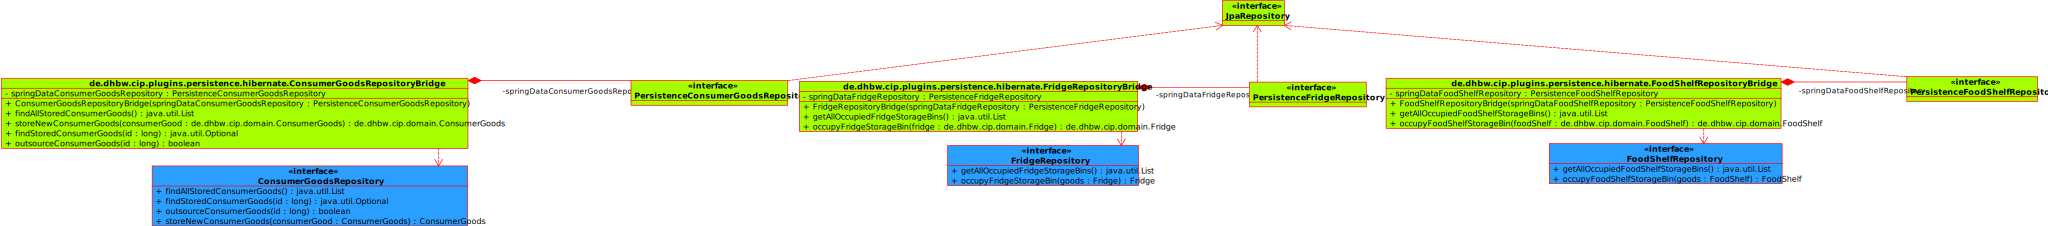
\includegraphics[width=1.0\textwidth]{Bilder/entwurfsmuster-bridge.pdf}
% 	\caption[Ausschnitt des UML-Diagramms zur Darstellung des \textit{Bridge}-Entwurfmusters.]{Der Ausschnitt des UML-Diagramms verdeutlicht die Verwendung des \textit{Bridge}-Entwurfmusters.}
% 	\label{fig:uml-bridge-pattern}
% \end{figure}

% \begin{figure}[H]
% 	\centering
% 	\includegraphics[width=1.0\textwidth]{Bilder/entwurfsmuster-factory.pdf}
% 	\caption[Ausschnitt des UML-Diagramms zur Darstellung des \textit{Builder}-Entwurfmusters.]{Der Ausschnitt des UML-Diagramms verdeutlicht die Verwendung des \textit{Builder}-Entwurfmusters.}
% 	\label{fig:uml-builder-pattern}
% \end{figure}

\subsection*{\code{Builder}-Entwurfsmuster}
Das \code{Builder}-Entwurfsmuster zählt zu den \textit{Erzeugungsmustern} und ist in der Klasse \href{https://github.com/lucasmerkel/dhbw-advancedswe-programmentwurf/blob/d5c89113d12c3b877ddc4d6a99225b277ddd468f/swe_programmentwurf/consumergoods-inventory-planner/3-cip-domain/src/main/java/de/dhbw/cip/domain/ConsumerGoods.java#L72}{\code{ConsumerGoodsBuilder}} umgesetzt.
An dieser Stelle wurde ein \code{Builder}-Entwurfsmuster eingesetzt, da es die Möglichkeit gibt, nötige Attribute zu sammeln und, im Gegensatz zum direkten Erzeugen eines Objekts, die Möglichkeit der Überprüfung aufGültigkeit der Attribute vor dem Erzeugen des Objekts ermöglicht.
Der Einsatz ist in diesem Fall sinnvoll, da neben dem Abfangen von Fehlern bei der fehlenden Übertragung von Attributen, Datumseingaben oder Werteeingaben auf Gültigkeit überprüfen zu sind.

Das \code{Bridge}-Entwurfsmuster zählt zu den \textit{Strukturmustern} und ist in den Klassen \href{https://github.com/lucasmerkel/dhbw-advancedswe-programmentwurf/blob/d5c89113d12c3b877ddc4d6a99225b277ddd468f/swe_programmentwurf/consumergoods-inventory-planner/0-cip-plugins/src/main/java/de/dhbw/cip/plugins/persistence/hibernate/ConsumerGoodsRepositoryBridge.java}{\code{ConsumerGoodsRepositoryBridge}}, \href{https://github.com/lucasmerkel/dhbw-advancedswe-programmentwurf/blob/d5c89113d12c3b877ddc4d6a99225b277ddd468f/swe_programmentwurf/consumergoods-inventory-planner/0-cip-plugins/src/main/java/de/dhbw/cip/plugins/persistence/hibernate/FridgeRepositoryBridge.java}{\code{FridgeRepositoryBridge}} sowie \href{https://github.com/lucasmerkel/dhbw-advancedswe-programmentwurf/blob/d5c89113d12c3b877ddc4d6a99225b277ddd468f/swe_programmentwurf/consumergoods-inventory-planner/0-cip-plugins/src/main/java/de/dhbw/cip/plugins/persistence/hibernate/FoodShelfRepositoryBridge.java}{\code{FoodShelfRepositoryBridge}} umgesetzt.
Das \code{Bridge}-Entwurfsmuster wurde eingesetzt, da es die Trennung der Domänenlogik von der Pluginlogik ermöglicht.
Während die Repository-Interfaces \href{}{\code{ConsumerGoodsRepository}}, \href{}{\code{FridgeRepository}} und \href{}{\code{FoodShelfRepository}} zur Domäne zählen, findet die Persistierung der Objekte über ein Plugin mit der Implementierung der Interfaces \href{https://github.com/lucasmerkel/dhbw-advancedswe-programmentwurf/blob/d5c89113d12c3b877ddc4d6a99225b277ddd468f/swe_programmentwurf/consumergoods-inventory-planner/0-cip-plugins/src/main/java/de/dhbw/cip/plugins/persistence/hibernate/PersistenceConsumerGoodsRepository.java}{\code{PersistenceConsumerGoodsRepository}}, \href{https://github.com/lucasmerkel/dhbw-advancedswe-programmentwurf/blob/d5c89113d12c3b877ddc4d6a99225b277ddd468f/swe_programmentwurf/consumergoods-inventory-planner/0-cip-plugins/src/main/java/de/dhbw/cip/plugins/persistence/hibernate/PersistenceFridgeRepository.java}{\code{PersistenceFridgeRepository}} sowie \href{https://github.com/lucasmerkel/dhbw-advancedswe-programmentwurf/blob/d5c89113d12c3b877ddc4d6a99225b277ddd468f/swe_programmentwurf/consumergoods-inventory-planner/0-cip-plugins/src/main/java/de/dhbw/cip/plugins/persistence/hibernate/PersistenceFoodShelfRepository.java}{\code{PersistenceFoodShelfRepository}} statt.
Durch Anwenden des \code{Bridge}-Entwurfsmuster ist es nun möglich, auf einen implementierten Typ des entsprechenden Repository-Interfaces für die Interaktion mit der Entitätsverwaltung zuzugreifen.
Das \code{Bridge}-Entwurfsmuster hat das entsprechende Repository-Interface implementiert und übernimmt die Kommunikation mit dem Persistierungs-Plugin.
Somit ist die Aufteilung entsprechend der \textit{Clean Architecture} gewährleistet und bei einem Austausch des Persistierungs-Plugins bedarf nur Änderungen in der \textit{Plugin}-Schicht, während das Repository-Interface in der \textit{Domänen}-Schicht sowie alle darauf zugreifenden Instanzen davon unberührt sind.

\include{Inhalt/04_Inhalt/Refactoring}
%\include{Inhalt/04_Inhalt/einleitung}
%\include{Inhalt/04_Inhalt/formatText}
%\include{Inhalt/04_Inhalt/abbildungen}
%\include{Inhalt/04_Inhalt/mathematische-formeln}
%\include{Inhalt/04_Inhalt/quellcode}
%\include{Inhalt/04_Inhalt/literaturHinweis}

% ---- Literaturverzeichnis
\cleardoublepage
\renewcommand*{\chapterpagestyle}{plain}
\pagestyle{plain}
\pagenumbering{Roman}                   % Römische Seitenzahlen
\setcounter{page}{\numexpr\value{savepage}+1}
\printbibliography[title=Literaturverzeichnis]

% ---- Anhang
\appendix
%\clearpage
%\pagenumbering{Roman}  % römische Seitenzahlen für Anhang

\newpage
\end{document}
